%%%%%%%%%%%%%%%%%%%%%%%%%%%%%%%%%%%%%%%%%%%%%%%%%%%%%%%%%%%%%%%%%%%%
%% I, the copyright holder of this work, release this work into the
%% public domain. This applies worldwide. In some countries this may
%% not be legally possible; if so: I grant anyone the right to use
%% this work for any purpose, without any conditions, unless such
%% conditions are required by law.
%%%%%%%%%%%%%%%%%%%%%%%%%%%%%%%%%%%%%%%%%%%%%%%%%%%%%%%%%%%%%%%%%%%%

\documentclass[9pt]{beamer}
\usetheme[faculty=fi]{fibeamer}
\usepackage[utf8]{inputenc}
\usepackage[
  main=english, %% By using `czech` or `slovak` as the main locale
                %% instead of `english`, you can typeset the
                %% presentation in either Czech or Slovak,
                %% respectively.
  % czech, slovak %% The additional keys allow foreign texts to be
]{babel}        %% typeset as follows:
%%
%%   \begin{otherlanguage}{czech}   ... \end{otherlanguage}
%%   \begin{otherlanguage}{slovak}  ... \end{otherlanguage}
%%
%% These macros specify information about the presentation
\title{Neutrino Flavor Conversions in Dense Medium: Matter Stimulation, Dispersion Relation, and Neutrino Halo} %% that will be typeset on the
\author{Lei Ma\\ Supervisor: Huaiyu Duan}
\subtitle{PhD Defense} %% title page.

%% These additional packages are used within the document:
\usepackage{ragged2e}  % `\justifying` text
\usepackage{booktabs}  % Tables
\usepackage{tabularx}
\usepackage{tikz}      % Diagrams
\usetikzlibrary{calc, shapes, backgrounds}
\usepackage{amsmath, amssymb}
\usepackage{url}       % `\url`s
\usepackage{listings}  % Code listings

% \usepackage{appendixnumberbeamer}


\usepackage[T1]{fontenc}
% \usefonttheme[onlymath]{serif}
\renewcommand\sfdefault{cmbr}



%\usepackage{booktabs}
%\usepackage[scale=2]{ccicons}
\usepackage{tcolorbox}

%\usepackage{floatrow}

%\usepackage{minted}
%\usemintedstyle{trac}

% For the 68 colors
\usepackage{xcolor}
\definecolor{ao}{rgb}{0.0, 0.5, 0.0}

% \usepackage{pgfplots}
% \usepgfplotslibrary{dateplot}

% \usepackage{xspace}
% \newcommand{\themename}{\textbf{\textsc{metropolis}}\xspace}


\usepackage{subfig}
\usepackage[absolute
,overlay
]{textpos}

%%%%% eso-pic package that set up a grid system for the slides BEGIN
%\usepackage[texcoord,grid,gridcolor=red!10,subgridcolor=green!10,gridunit=pt]{eso-pic}
% grid,gridcolor=red!20,subgridcolor=green!20,gridunit=pt
%%%%% eso-pic package that set up a grid system for the slides END

\usepackage{tikz}



\usepackage{times}
\usepackage{verbatim}
\usetikzlibrary{arrows,shapes}


\usepackage{mathtools}

\newcommand{\verteq}{\rotatebox{90}{$\,=$}}
\newcommand{\equalto}[2]{\underset{\scriptstyle\overset{\mkern4mu\huge \verteq}{#2}}{#1}}


\newcommand{\bra}[1]{\left\langle #1\right|}
\newcommand{\ket}[1]{\left| #1\right\rangle}
\newcommand{\braket}[2]{\langle #1 | #2 \rangle}
\newcommand{\avg}[1]{\left< #1 \right>}
\newcommand{\ii}{\mathrm{i}}
\DeclareMathOperator{\sech}{sech}



\frenchspacing
\begin{document}
  \frame{\maketitle}

%%%%%%%%%%%%%%%%%%%%%%%%%%%%%%%%%%%%%%%%%%%%%%
%%%%%%%%%%%%%%%%
  \AtBeginSection[]{% Print an outline at the beginning of sections
    \begin{frame}<beamer>
      \frametitle{Outline for Section \thesection}
      \tableofcontents[currentsection]
    \end{frame}}

%%%%%%%%%%% Dark Frames
  \begin{darkframes}


    \section{Neutrino Oscillations}

    \subsection{Neutrinos as Fundamental Particles}

    \begin{frame}{What are Neutrinos?}
      \begin{minipage}[\textheight]{\textwidth}
      \begin{columns}[T]

      \begin{column}{0.6\textwidth}
      \begin{figure}
      %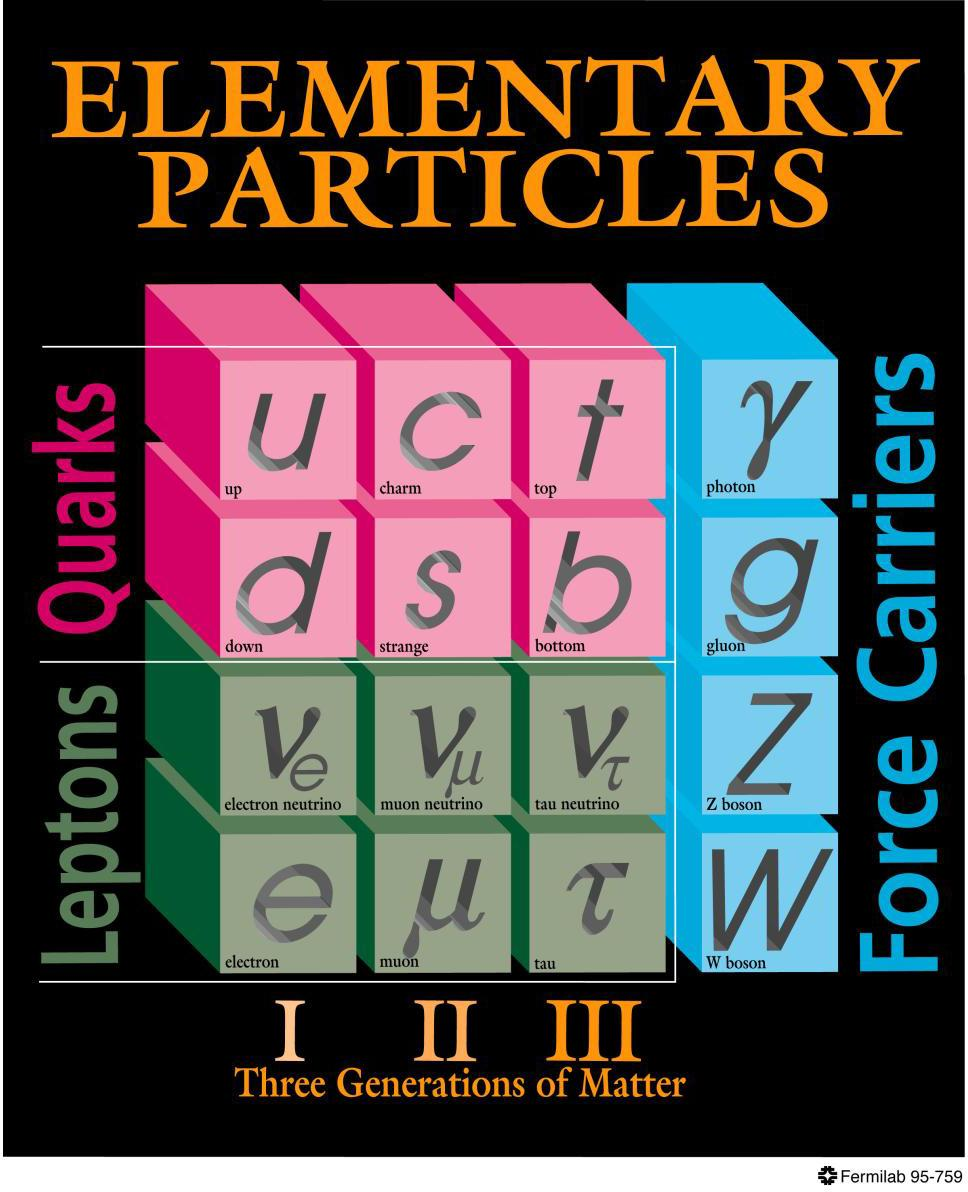
\includegraphics[width=0.9\linewidth,height=0.8\textheight,keepaspectratio]{assets/elementary-particles}
      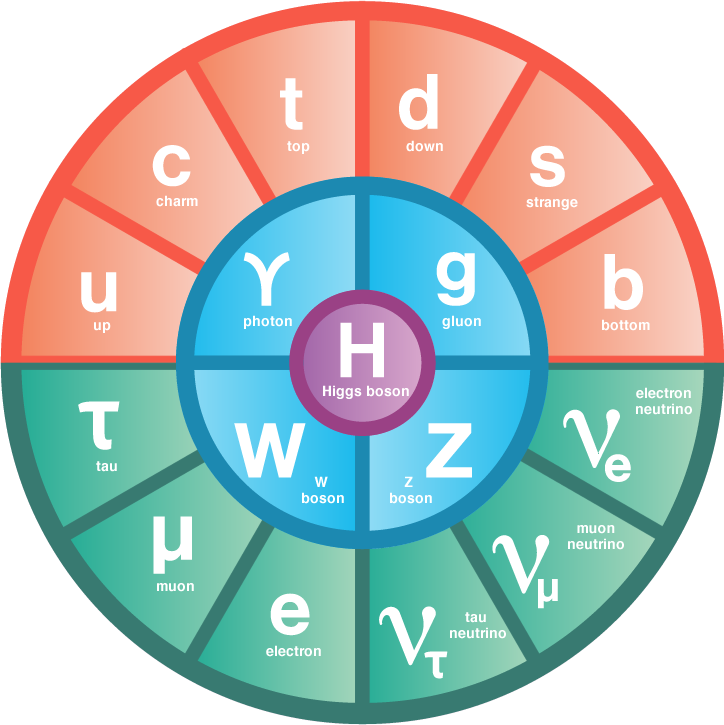
\includegraphics[width=0.9\linewidth,height=0.8\textheight,keepaspectratio]{assets/standard-model}
      \caption*{Elementary particles. \\ Source: symmetrymagazine.org} % http://www-d0.fnal.gov/Run2Physics/WWW/results/final/TOP/T06C/T06C.html
      \end{figure}
      \end{column}

      \begin{column}{0.4\textwidth}


          \begin{itemize}
          \item[] Neutrinos are
          \item fermions,
          \item electrically neutral,
          \item three flavors,
          \item none vanishing mass.
          \end{itemize}



      \only<1-1>{
      \begin{figure}
      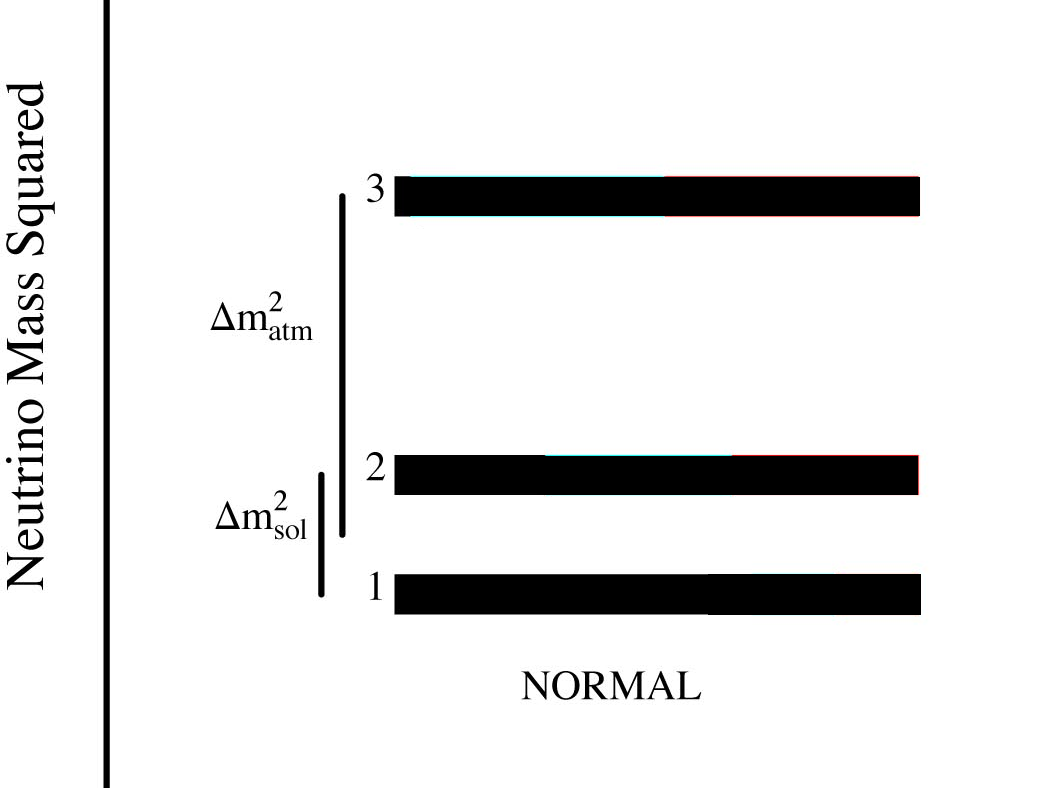
\includegraphics[width=\textwidth]{assets/neutrino-mass-normal-hierarchy-simple.png}
      \caption*{Adapted from Olga Mena \& Stephen Parke (2004)}
      \end{figure}
      }

      \only<2-2>{
      \begin{figure}
      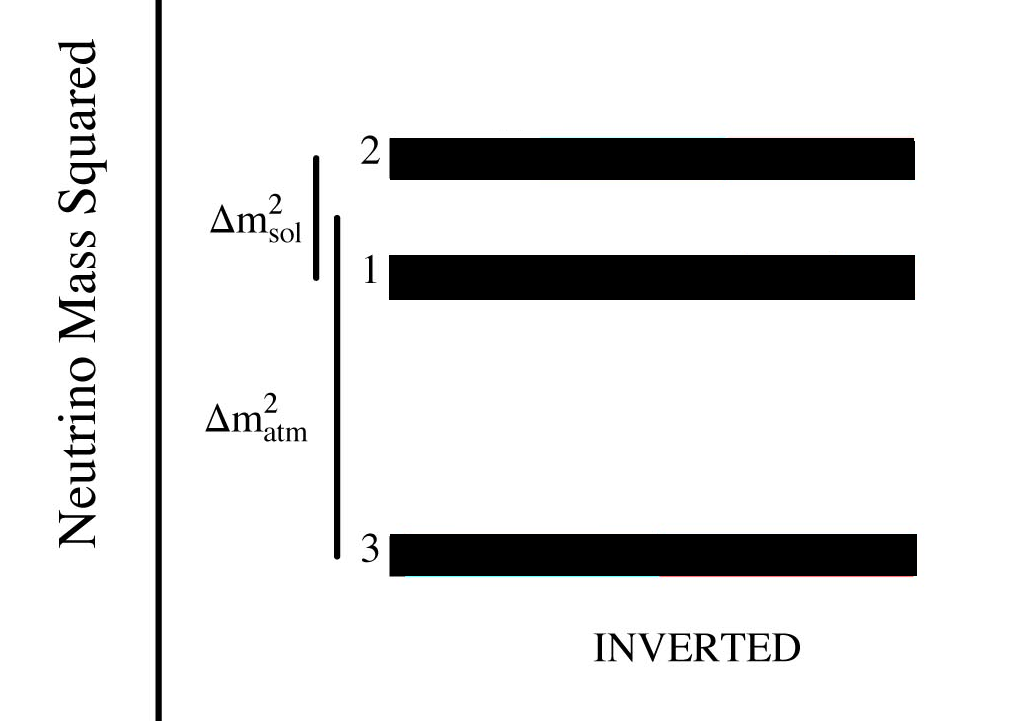
\includegraphics[width=\textwidth]{assets/neutrino-mass-inverted-hierarchy-simple.png}
      \caption*{Adapted from Olga Mena \& Stephen Parke (2004)}
      \end{figure}
      }

      \end{column}


      \end{columns}
      \end{minipage}

    \end{frame}


%%%%% Neutrino Oscillations %%%%%%%%%

\subsection{Why Do Neutrinos Oscillate}

% For every picture that defines or uses external nodes, you'll have to
% apply the 'remember picture' style. To avoid some typing, we'll apply
% the style to all pictures.
\tikzstyle{every picture}+=[remember picture]

% By default all math in TikZ nodes are set in inline mode. Change this to
% displaystyle so that we don't get small fractions.
\everymath{\displaystyle}


\begin{frame}{Why Do Neutrinos Oscillate?}

Flavor states are different from mass states.

\begin{equation*}
\begin{pmatrix}
\psi_e\\
\psi_\mu
\end{pmatrix} = \begin{pmatrix}
\cos \theta_{\mathrm v} & \sin\theta_{\mathrm v} \\
-\sin \theta_{\mathrm v} & \cos \theta_{\mathrm v}
\end{pmatrix}\begin{pmatrix}
\psi_1\\
\psi_2
\end{pmatrix}
\end{equation*}

\end{frame}



\begin{frame}[fragile]{Why Do Neutrinos Oscillate?}
\setbeamercovered{invisible}





\begin{tcolorbox}[title=Equation of Motion]

\begin{equation*}
i\partial_x \begin{pmatrix}
\psi_e\\
\psi_\mu
\end{pmatrix} = \mathbf{H}\begin{pmatrix}
\psi_e\\
\psi_\mu
\end{pmatrix}
\end{equation*}

\end{tcolorbox}

\pause

\begin{tcolorbox}
\begin{equation*}
\mathbf{H} = \frac{\omega_{\mathrm v} }{2}\left( - \cos 2\theta_{\mathrm v } \boldsymbol{\sigma}_3  + \sin 2\theta_{\mathrm{v}} \boldsymbol{\sigma}_1\ \right)
\end{equation*}


\begin{itemize}
    \item \color{black} Oscillation frequency:
\begin{equation*}
    \omega_{\mathrm v} = \frac{\delta m^2}{2E}=\frac{m_2^2 - m_1^2}{2E}
\end{equation*}
\item \color{black} Mixing angle $\theta_{\mathrm v}$
\end{itemize}


\end{tcolorbox}






\end{frame}



\begin{frame}{Flavor Isospin}
\setbeamercovered{invisible}








\begin{columns}[T]
\begin{column}{0.5\textwidth}


Hamiltonian: $\mathbf H = - \frac{\vec{\boldsymbol{\sigma}} }{2}\cdot \vec H$


Flavor isospin: $\vec s = \Psi^{\dagger} \frac{\vec{\boldsymbol{\sigma}} }{2} \Psi $

\small
Electron flavor survival probability
\vspace*{0pt}
\begin{equation*}
P = \frac{1}{2} + s_3
\end{equation*}


Equation of motion

\begin{equation*}
\dot{\vec s} = \vec s \times \vec H
\end{equation*}




\end{column}%
\begin{column}{0.5\textwidth}

\begin{tcolorbox}
\begin{figure}
    \centering
    % \vspace*{-10pt}
    \includegraphics[width=\textwidth]{assets/flavor-isospin-illus}
\end{figure}
\end{tcolorbox}

\end{column}
\end{columns}

\pause


\begin{columns}[T]
\begin{column}{0.5\textwidth}
\vspace{10pt}
Vacuum oscillation Hamiltonian

\begin{align*}
&\frac{\omega_{\mathrm v} }{2}\left( - \cos 2\theta_{\mathrm v } \boldsymbol{\sigma}_3  + \sin 2\theta_{\mathrm{v}} \boldsymbol{\sigma}_1\ \right)\\
\to & \cos 2\theta_{\mathrm v}\begin{pmatrix}
0\\
0\\
\omega_{\mathrm v}
\end{pmatrix} -\sin 2\theta_{\mathrm v}\begin{pmatrix}
\omega_{\mathrm v}\\
0\\
0
\end{pmatrix}
\end{align*}



\end{column}%
\begin{column}{0.5\textwidth}

\begin{tcolorbox}
\begin{figure}
    \centering
    % \vspace*{-20pt}
    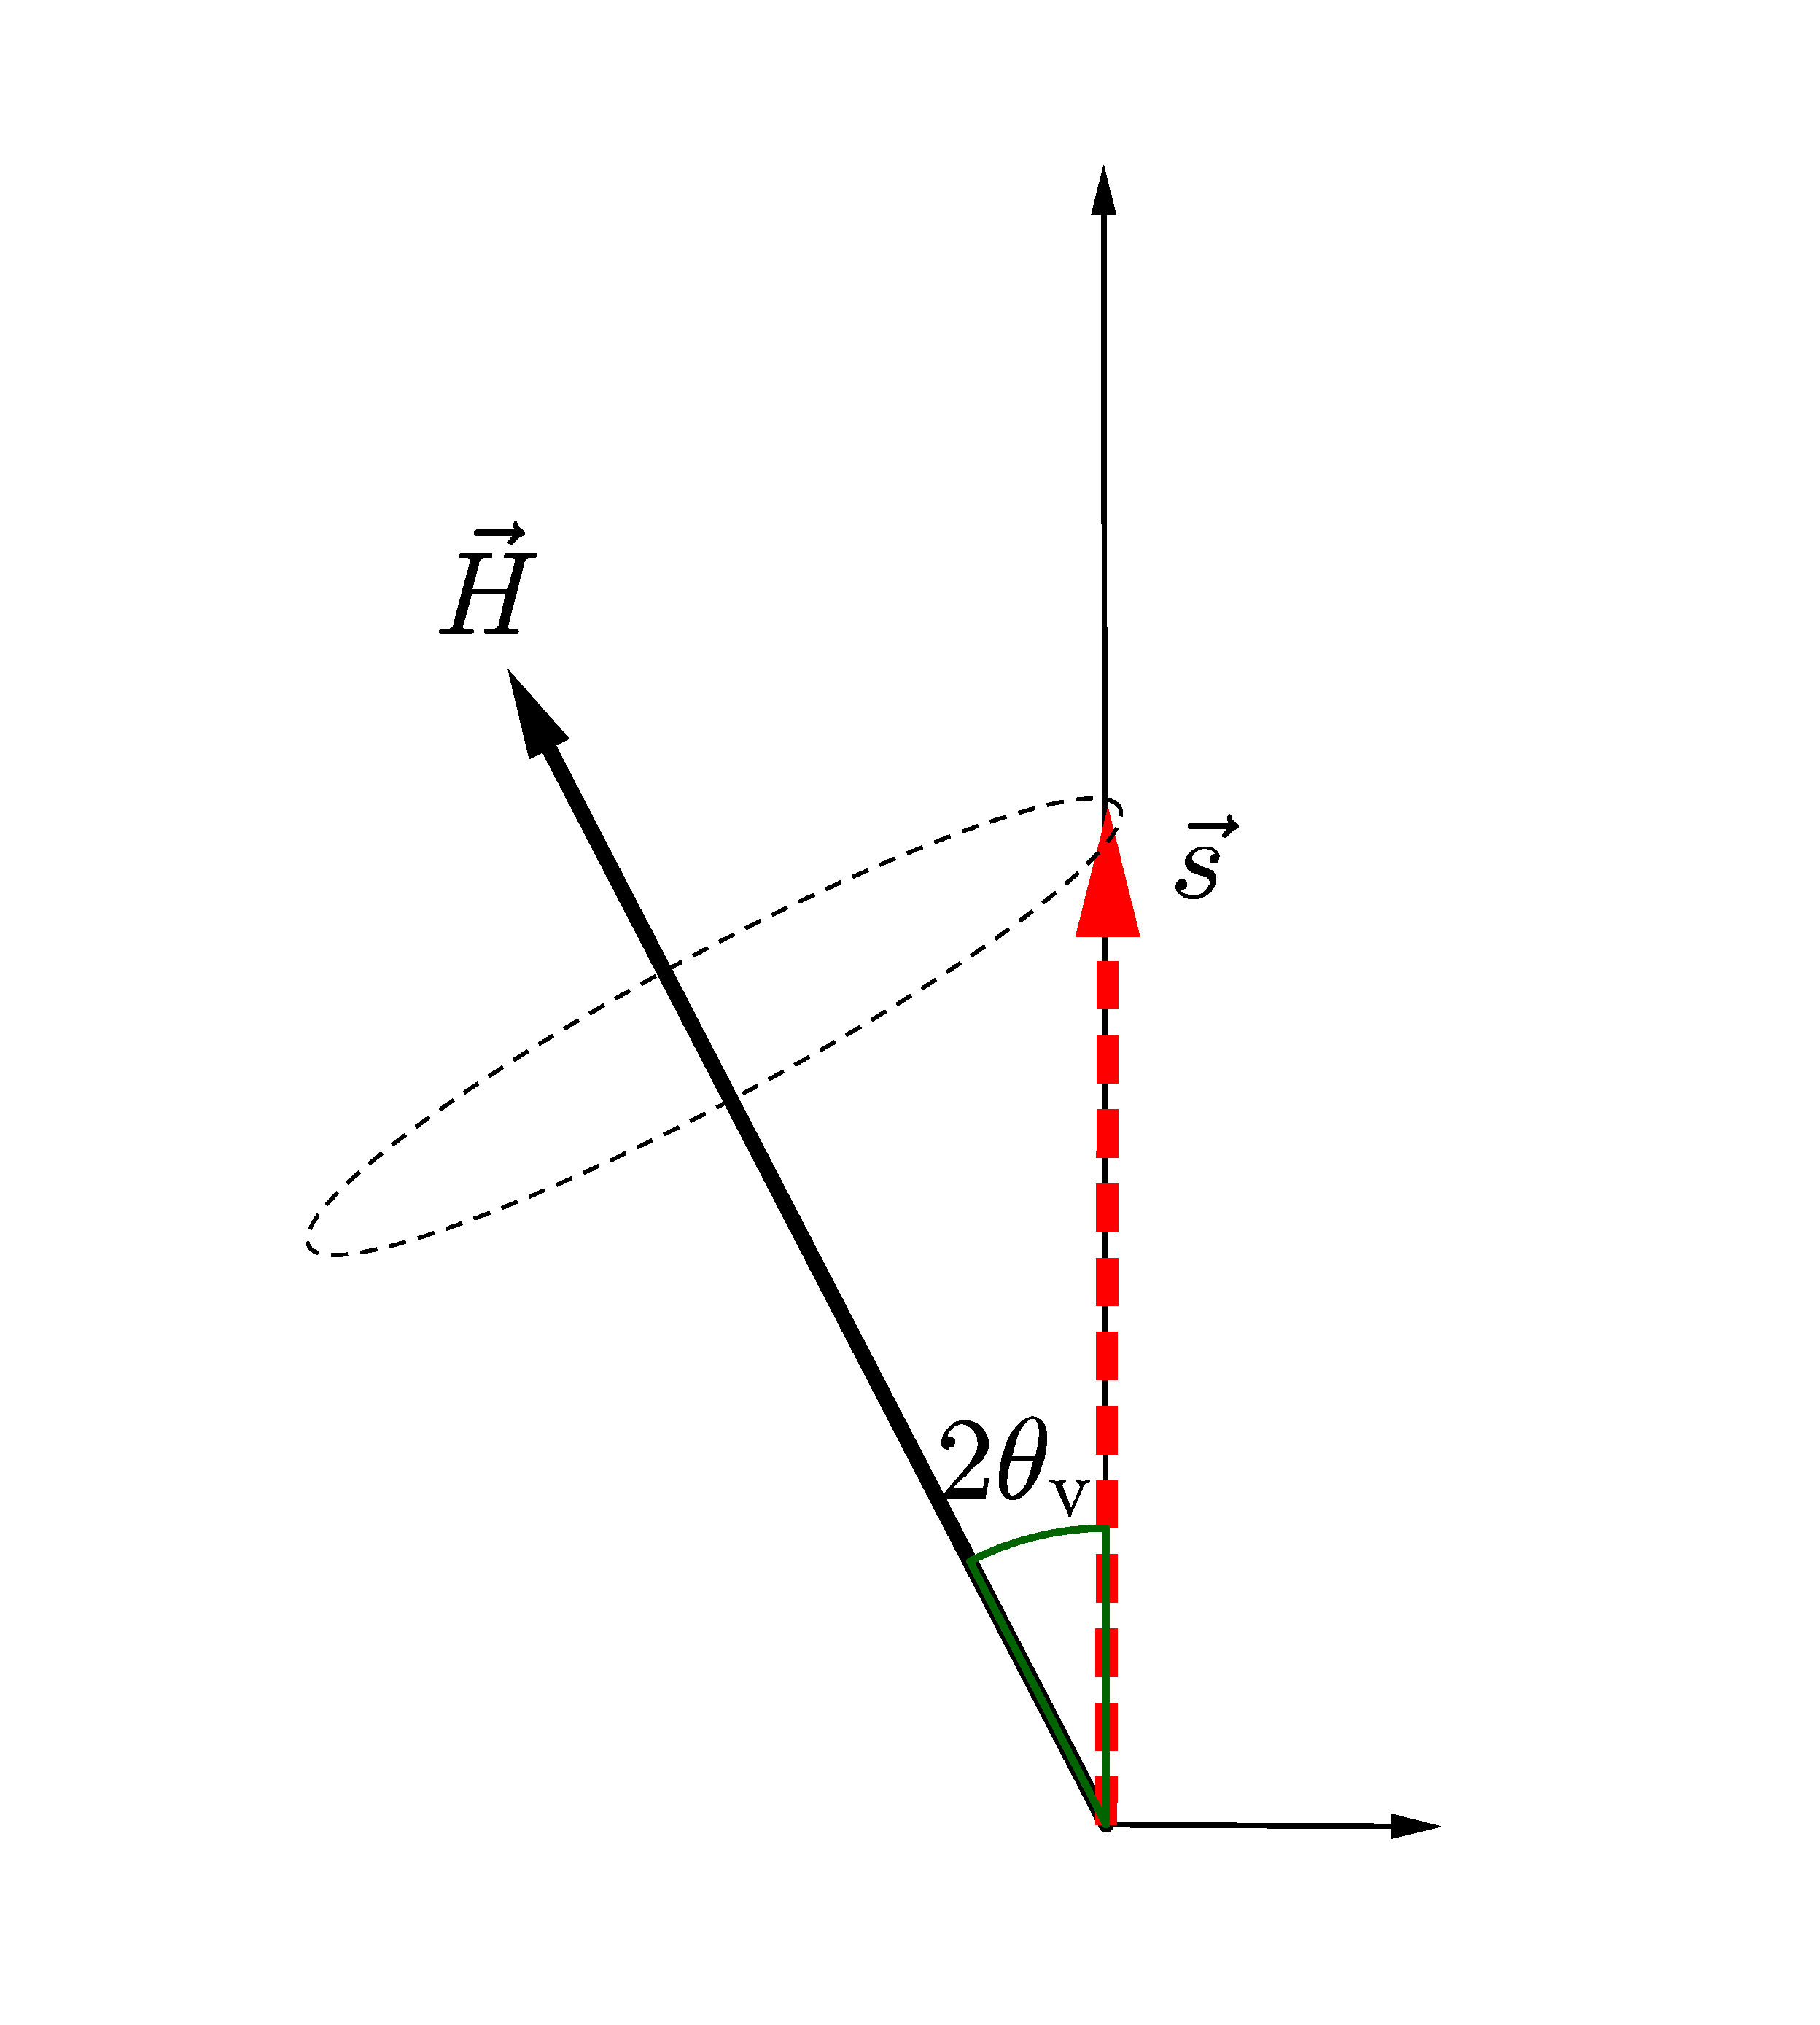
\includegraphics[width=0.7\textwidth]{assets/flavor-isospin-1}
\end{figure}
\end{tcolorbox}



\end{column}
\end{columns}




\end{frame}



%%%%%%%%%%%%%%%%%%%%%%%%%%%%%%%%%%%%%%%%%%%%%%%%%%%%%%%%%%%%%%%%%%
%%%%%%%%%%%%%%%%%%%% Matter Effect %%%%%%%%%%%%%%%


\section{Matter Stimulated Oscillations}


\subsection{Matter Interactions, MSW Effect, and Solar Neutrino Problem}


\begin{frame}{Matter Interaction}


% \begin{tcolorbox}[title=PLACEHOLDER]
% SHOULD ADD IN WHY MATTER INTERACTION IS LIKE THIS.
% \end{tcolorbox}

\begin{tcolorbox}
\begin{figure}[ht]
\centering
\begin{minipage}[b]{0.45\linewidth}
\centering
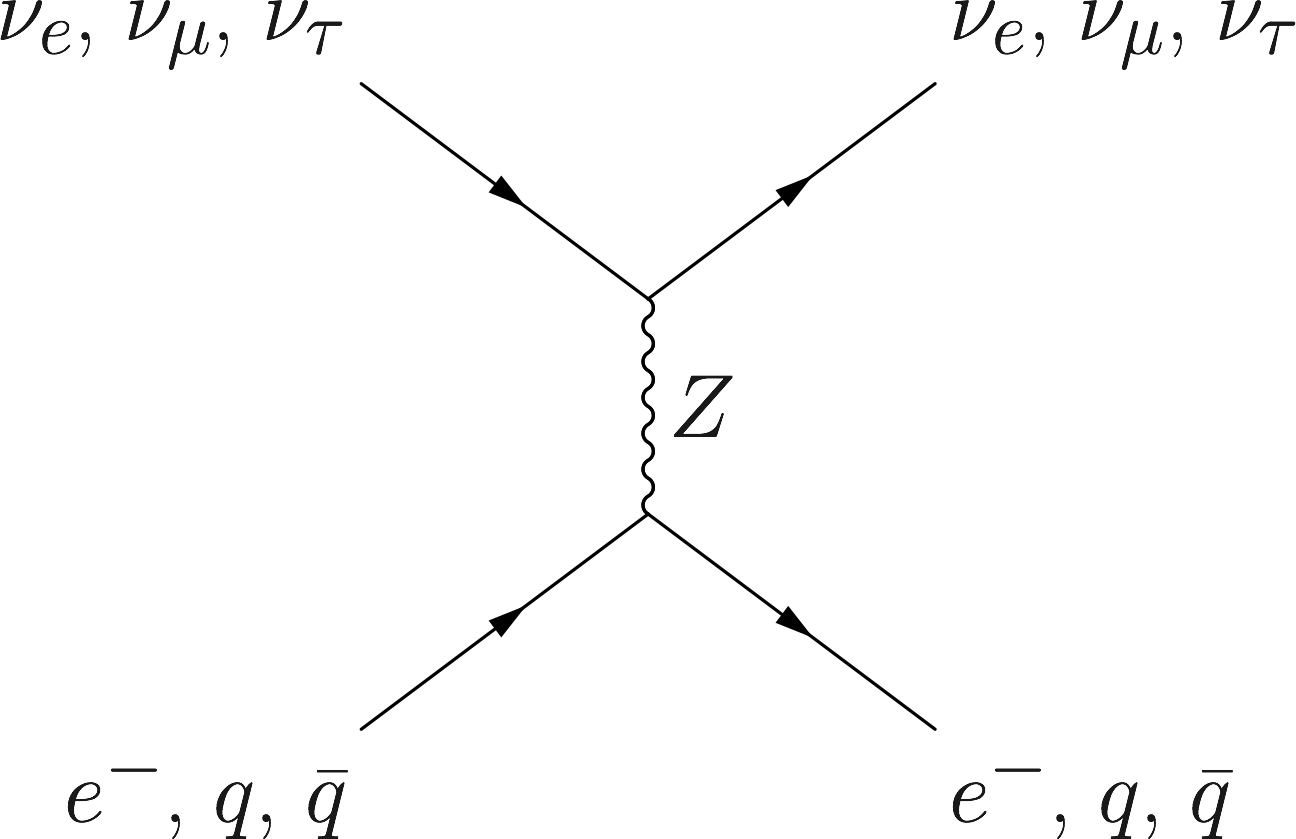
\includegraphics[height=0.32\textheight]{assets/neutral-current.png}
\caption*{\color{black}Neutral current interaction between $\nu_{\mathrm e}$, $\nu_{\mu}$, $\nu_{\tau}$,
and $e^{-}$, etc.}
\end{minipage}%
\begin{minipage}[b]{0.45\linewidth}
\centering
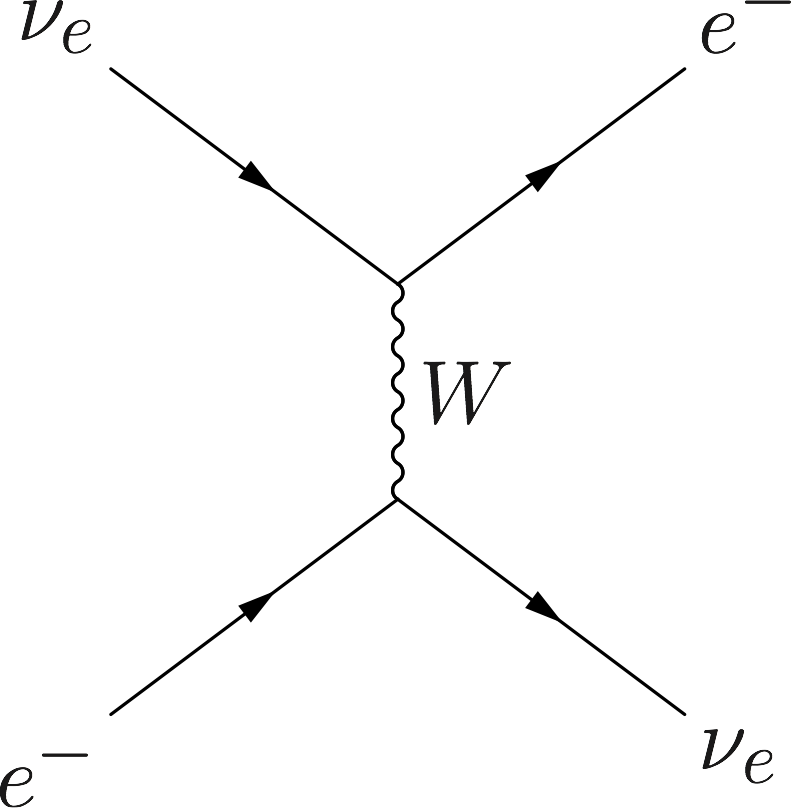
\includegraphics[height=0.32\textheight]{assets/charged-current.png}
\caption*{
\color{black}Charged current interaction between $\nu_{\mathrm e}$ and $e^{-}$}
\end{minipage}
\end{figure}

\end{tcolorbox}


\end{frame}





% For every picture that defines or uses external nodes, you'll have to
% apply the 'remember picture' style. To avoid some typing, we'll apply
% the style to all pictures.
\tikzstyle{every picture}+=[remember picture]


% By default all math in TikZ nodes are set in inline mode. Change this to
% displaystyle so that we don't get small fractions.
\everymath{\displaystyle}







% For every picture that defines or uses external nodes, you'll have to
% apply the 'remember picture' style. To avoid some typing, we'll apply
% the style to all pictures.
\tikzstyle{every picture}+=[remember picture]


% By default all math in TikZ nodes are set in inline mode. Change this to
% displaystyle so that we don't get small fractions.
\everymath{\displaystyle}



\begin{frame}{Matter Interaction}
\setbeamercovered{invisible}

\tikzstyle{na} = [baseline=-.5ex]




\begin{itemize}
    \item[] Hamiltonian with matter interaction in flavor basis  ($\omega_{\mathrm{v}}=\delta m^2/2E$):
        \tikz[na] \node[coordinate] (n1) {};
\end{itemize}




\only<1->{
\begin{equation*}
    \mathbf{H} =
    \tikz[baseline]{
            \node[fill=blue!50,anchor=base] (t1)
            {$ \frac{\omega_{\mathrm{v}}}{2}\left( - \cos 2\theta_{\mathrm{v}} \boldsymbol{\sigma_3} + \sin 2\theta_{\mathrm{v}} \boldsymbol{\sigma_1} \right) $}
            }
            \tikz[baseline]{
            \node[fill=red!50, anchor=base] (t2)
            {$
            +\frac{\lambda(x)}{2} \boldsymbol{\sigma_3}
            $};
        }
\end{equation*}

}


\begin{itemize}
    \item Vacuum Hamiltonian
        \tikz[na]\node [coordinate] (n2) {};
    \item Matter interaction
        \tikz[na]\node [coordinate] (n3) {};
    \item<1-> $\lambda(x) = \sqrt{2}G_{\mathrm{F}} n_{\mathrm{e}}(x)$
\end{itemize}





% Now it's time to draw some edges between the global nodes. Note that we
% have to apply the 'overlay' style.
\begin{tikzpicture}[overlay]
        \path[->]<1-> (n2) edge [bend right] (t1);
        \path[->]<1-> (n3) edge [bend right=20] (t2);
\end{tikzpicture}




\end{frame}




% \subsection{MSW Effect}

\begin{frame}{MSW Effect}

\begin{align*}
    \mathbf H =& \colorbox{blue!50}{$ \frac{\omega_{\mathrm{v}}}{2}\left( - \cos 2\theta_{\mathrm{v}} \boldsymbol{\sigma_3} + \sin 2\theta_{\mathrm{v}} \boldsymbol{\sigma_1} \right) $}   \colorbox{red!50}{$ + \frac{\lambda(x)}{2} \boldsymbol{\sigma_3} $} \\
    \to &  \colorbox{blue!50}{$ \omega_{\mathrm v}\begin{pmatrix}
    - \sin 2\theta_{\mathrm v} \\
    0 \\
    \cos 2\theta_{\mathrm v}
\end{pmatrix} $}  \colorbox{red!50}{$ + \begin{pmatrix}
    0\\
    0\\
    - \lambda(x)
    \end{pmatrix} $} \\
    = &  \colorbox{blue!50}{$ \vec H_{\mathrm v} $}  \colorbox{red!50}{$ + \vec H_{\mathrm m}(x) $}
\end{align*}






\end{frame}


%%%%%%%%%%%%%%%%%

% \subsection{MSW Effect}

\begin{frame}{MSW Effect}

\only<1>{


\begin{columns}[T]
\begin{column}{0.5\textwidth}


\begin{figure}
    \centering
    \colorbox{white}{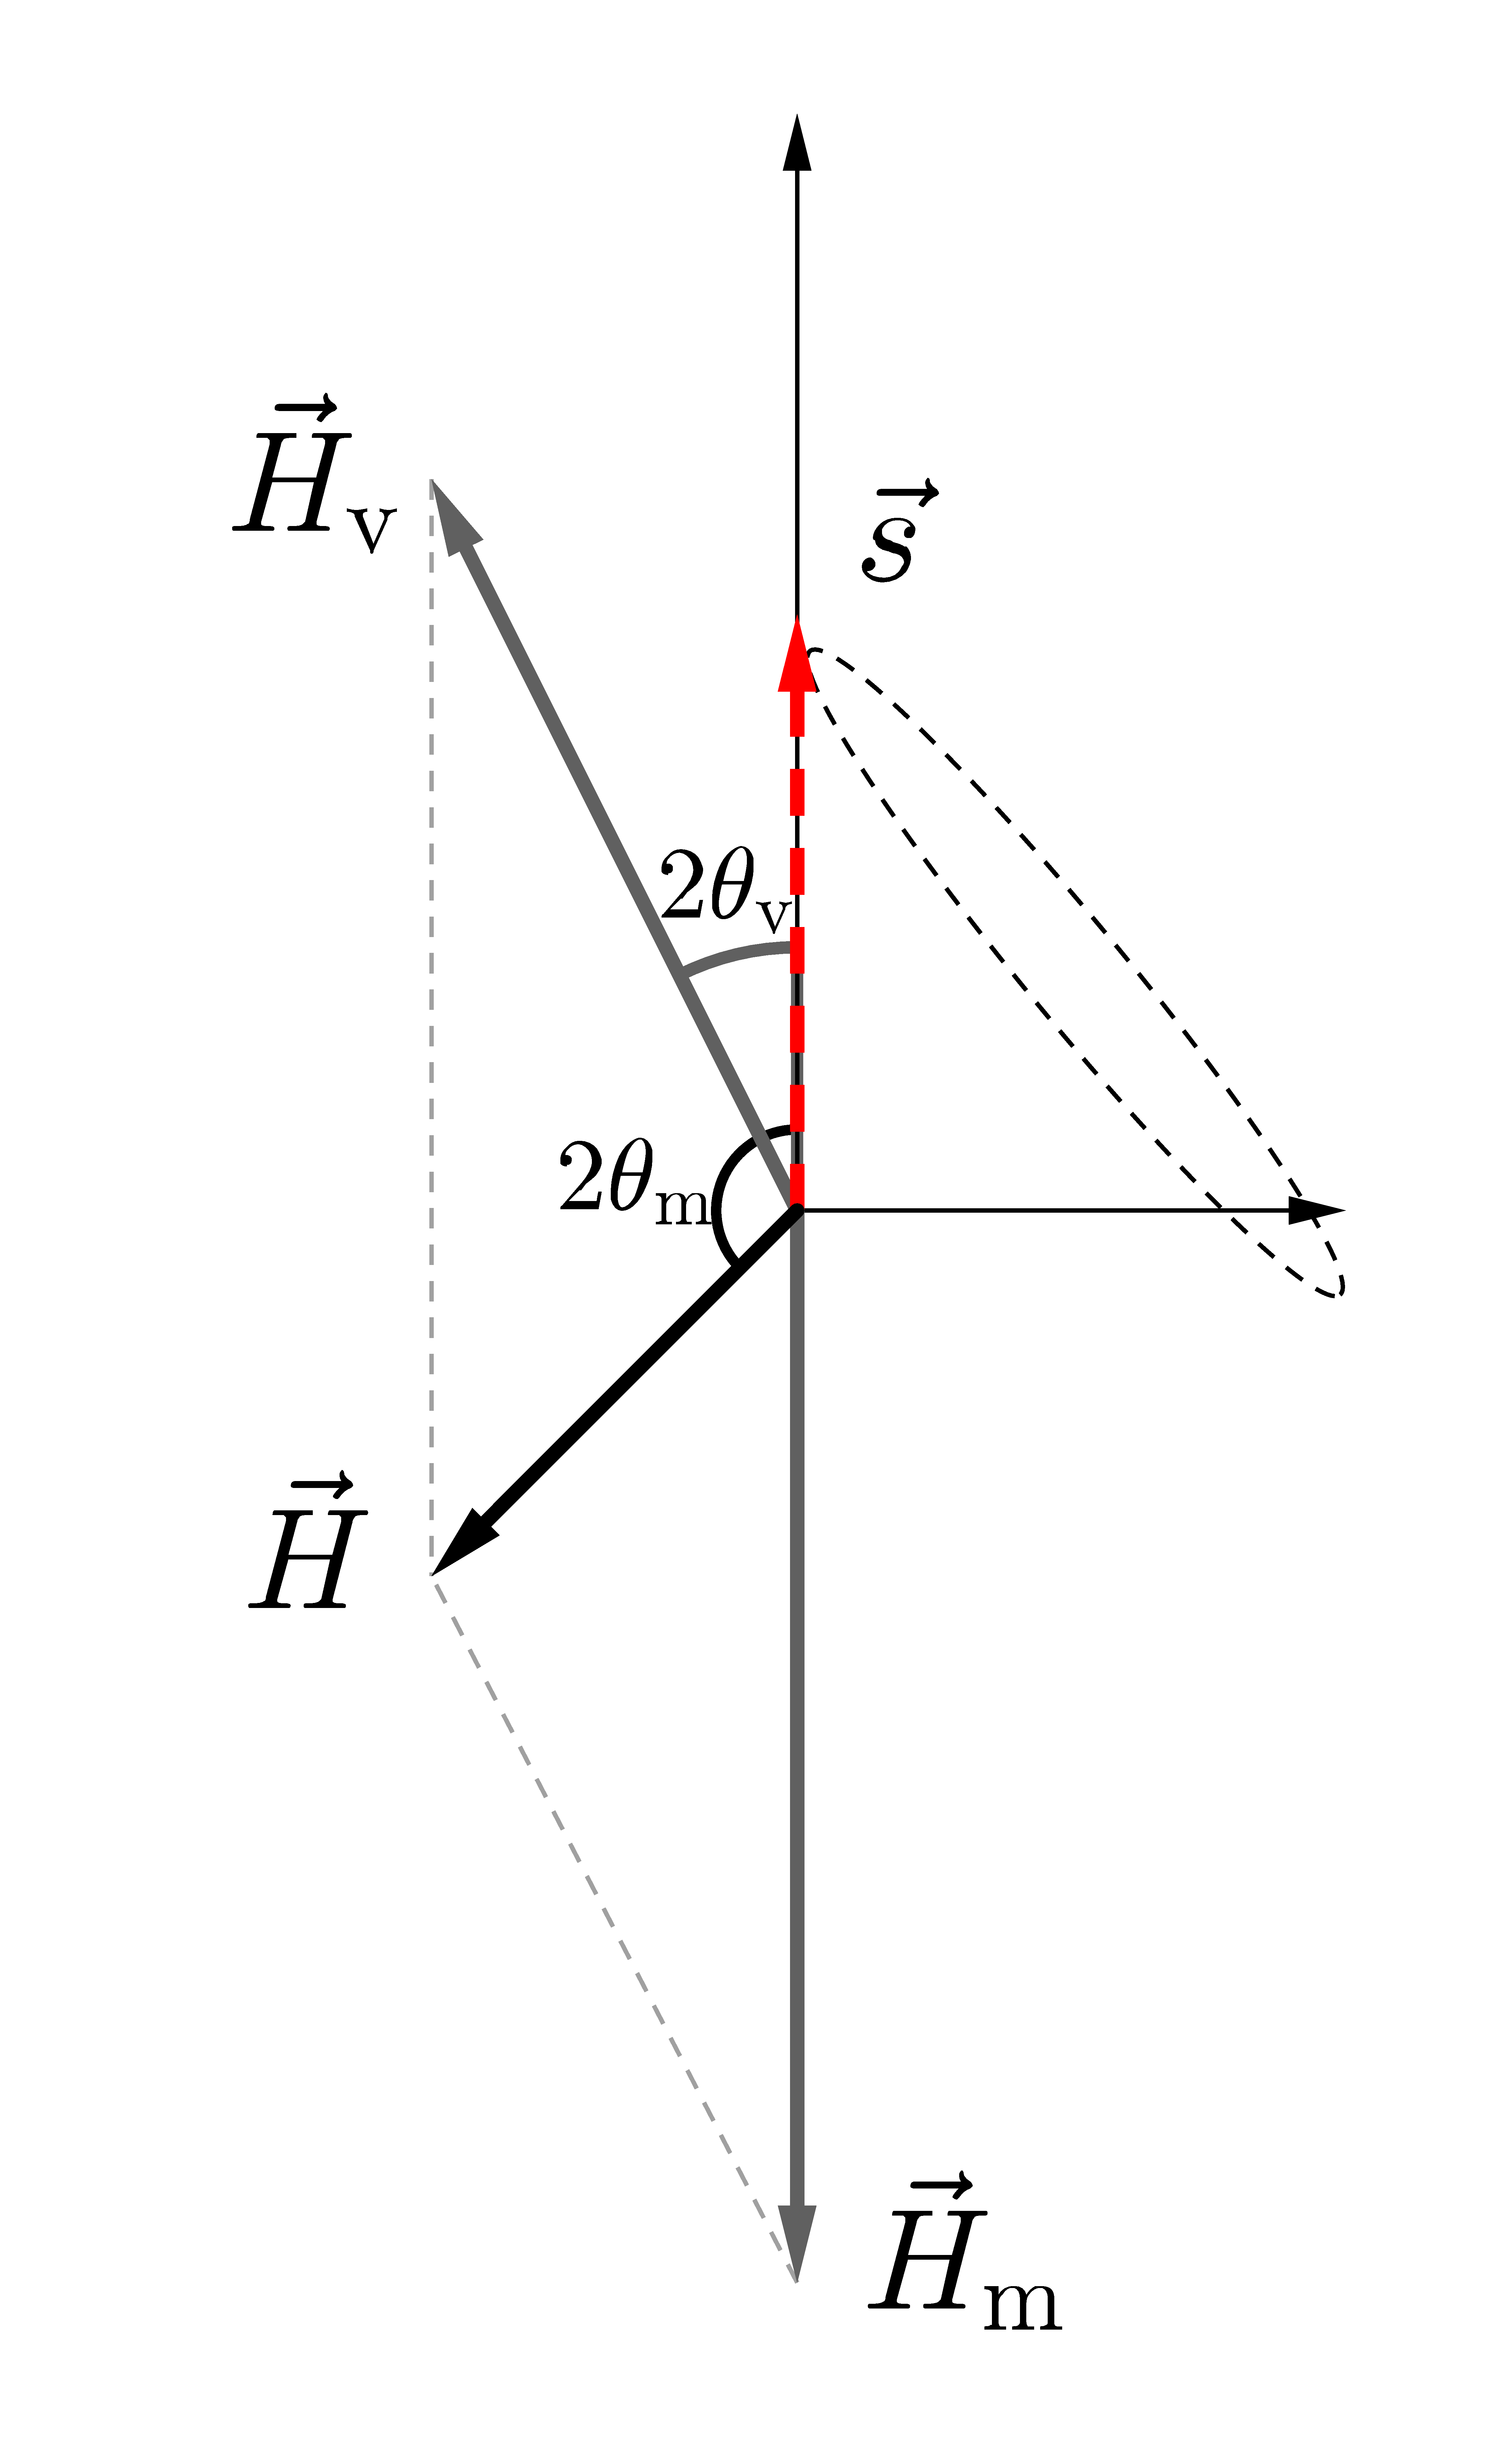
\includegraphics[width=0.9\textwidth]{assets/matter-effect-notsolarge-density}}
\end{figure}


\end{column}%
\begin{column}{0.5\textwidth}



Electron flavor survival probability

\begin{equation*}
P = \frac{1}{2} + s_3
\end{equation*}

Oscillation frequency in {\bf vacuum}:

\begin{equation*}
    \omega_{\mathrm v} = \lvert \vec H_{\mathrm v} \rvert
\end{equation*}


Oscillation frequency in {\bf matter}:

\begin{equation*}
    \omega_{\mathrm m} = \lvert \vec H \rvert
\end{equation*}

Flavor states and mass states in matter

\begin{equation*}
\begin{pmatrix}
\psi_e\\
\psi_\mu
\end{pmatrix} = \begin{pmatrix}
\cos \theta_{\mathrm m} & \sin\theta_{\mathrm m} \\
-\sin \theta_{\mathrm m} & \cos \theta_{\mathrm m}
\end{pmatrix}\begin{pmatrix}
\psi_{\mathrm L}\\
\psi_{\mathrm H}
\end{pmatrix}
\end{equation*}


\end{column}
\end{columns}


}

\only<2>{

\centering

Adiabatic matter density change

\begin{columns}[T]
\begin{column}{0.33\textwidth}

\begin{textblock*}{70pt}(50pt,50pt)
\small
Large density
\end{textblock*}



\begin{textblock*}{70pt}(280pt,50pt)
\small
Low density
\end{textblock*}



\begin{figure}
    \centering
    \colorbox{white}{\includegraphics[width=0.7\textwidth]{assets/matter-effect-large-density}}
\end{figure}


\end{column}%
\begin{column}{0.33\textwidth}



\begin{figure}
    \centering
    \colorbox{white}{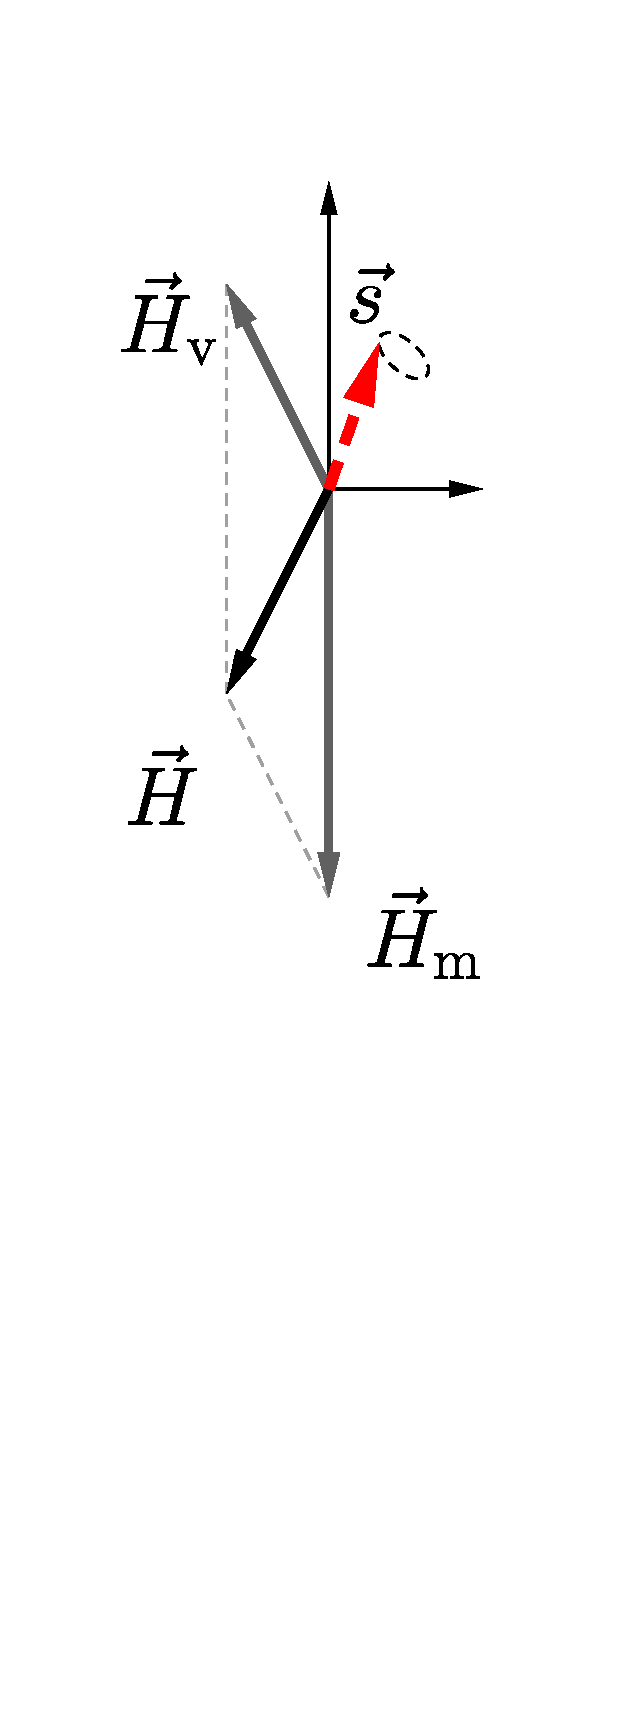
\includegraphics[width=0.6\textwidth]{assets/matter-effect-adiabatic}}
\end{figure}



\end{column}
\begin{column}{0.33\textwidth}



\begin{figure}
    \centering
    \colorbox{white}{\includegraphics[width=0.6\textwidth]{assets/matter-effect-adiabatic-3}}
\end{figure}



\end{column}
\end{columns}

}

\only<3> {


\begin{columns}[T]
\begin{column}{0.5\textwidth}



\begin{figure}
    \centering
    \colorbox{white}{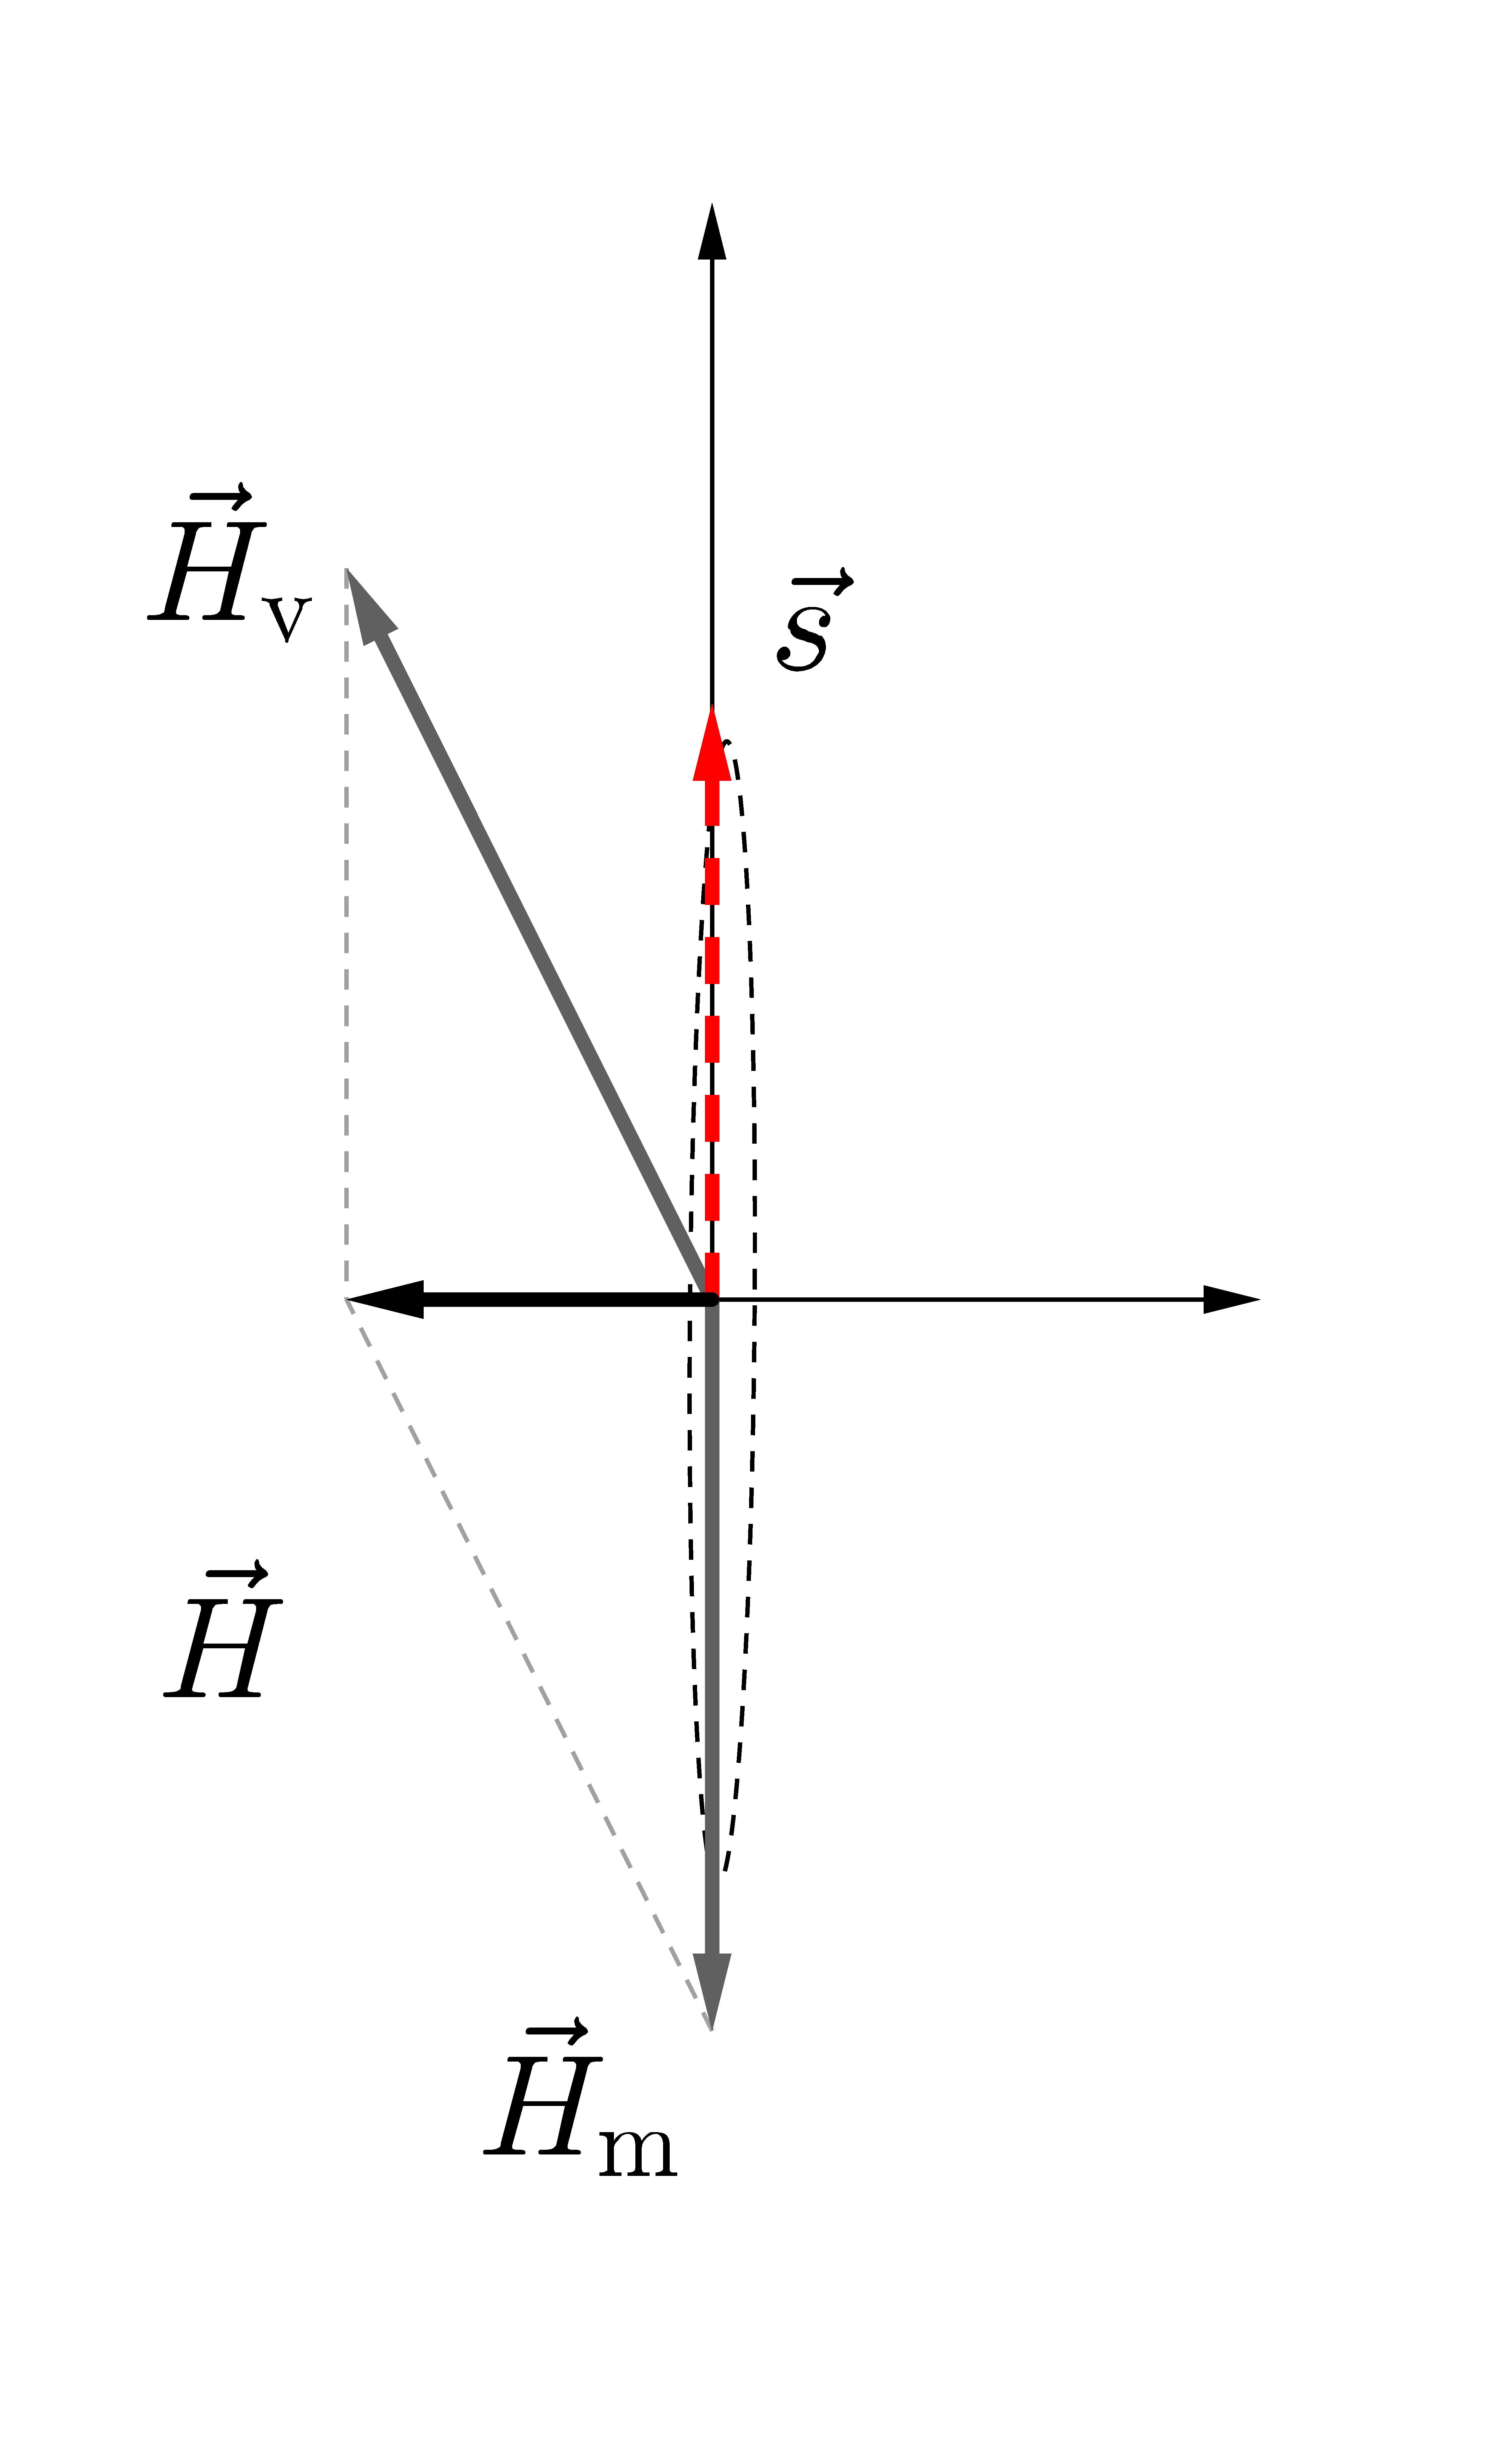
\includegraphics[width=0.9\textwidth]{assets/matter-effect-critical-density}}
\end{figure}


\end{column}%
\begin{column}{0.5\textwidth}



\begin{itemize}
\item
Maximum possible flavor transition probability amplitude
\item
MSW Resonance
\item
A specific matter density
\begin{equation*}
    \sqrt{2}G_{\mathrm F}n_{\mathrm e} \equiv \omega_{\mathrm v}\cos 2\theta_{\mathrm v}
\end{equation*}


\end{itemize}









\end{column}
\end{columns}


}




\end{frame}






%%%%%%% MSW Effect %%%%%%%%%

%\subsubsection{Solar Neutrino Problem}
%
% \begin{frame}{Solar Neutrino Problem}
%
%
% \begin{figure}
%     \centering
%     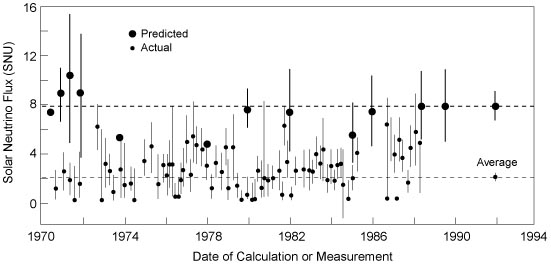
\includegraphics[width=0.9\textwidth]{assets/chlorine-detector-solar-neutrinos.jpg} %https://ase.tufts.edu/cosmos/print_images.asp?id=37
%     %https://ase.tufts.edu/cosmos/view_picture.asp?id=585
%     \caption*{Chlorine detector (Homestake experiment) results and theory predictions. SNU: 1 event for $10^{36}$ target atoms per second. Kenneth R. Lang (2010)}
% \end{figure}
%
%
% \end{frame}
%
%
% \begin{frame}{MSW Effect and Solar Neutrinos}
%
% % \setbeamercovered{invisible}
%
%
%
% \begin{equation*}
%     \mathbf{H} = \frac{\lambda(x) - \omega_{\mathrm v} \cos 2\theta_{\mathrm v}}{2} \boldsymbol{\sigma_3} + \frac{ \omega_{\mathrm v} \sin 2\theta_{\mathrm v}}{2} \boldsymbol{\sigma_1}
% \end{equation*}
%
%
% \begin{equation*}
% \begin{pmatrix}
% \ket{\nu_{\mathrm{L}}} \\
% \ket{\nu_{\mathrm{H}}}
% \end{pmatrix} =
% \begin{pmatrix}
% \cos\theta_{\mathrm m} & -\sin\theta_{\mathrm m} \\
% \sin\theta_{\mathrm m} & \cos\theta_{\mathrm m}
% \end{pmatrix}\begin{pmatrix}
% \ket{\nu_{\mathrm{e}}} \\
% \ket{\nu_{\mu}}
% \end{pmatrix}
% \end{equation*}
%
%
% \begin{equation*}
%     \mathbf{H}_{\text{matter-basis}} = -\frac{\omega_{\mathrm m}}{2}\boldsymbol{\sigma_3}
% \end{equation*}
%
%
%
% \begin{figure}
% \centering
% 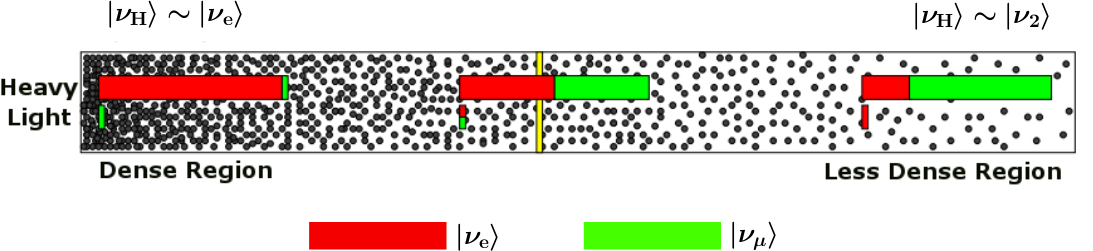
\includegraphics[width=0.9\textwidth]{assets/msw-and-density.png}
% \caption*{Yellow bar is the resonance point. Red: $\ket{\nu_e}$. Green: $\ket{\nu_\mu}$. Adapted from Smirnov, 2003.}
% \end{figure}
%
%
%
% \end{frame}
%
%
%
%
%
%
% \begin{frame}{MSW Effect}
%
%
% Suppose $\omega_{\mathrm v} = (m_2^2 - m_1^2)/2E <0$,
%
% \begin{equation*}
%     \mathbf{H} = \colorbox{blue!50}{$
%     -\frac{\omega_{\mathrm{v}}}{2}\begin{pmatrix} -\cos 2\theta_{\mathrm{v}} & \sin 2 \theta_{\mathrm{v}} \\ \sin 2\theta_{\mathrm{v}} & \cos 2\theta_{\mathrm{v}}  \end{pmatrix}
%     $}
%              \colorbox{red!50}{$
%             + \sqrt{2}G_{\mathrm{F}} n_{\mathrm{e}}(x) \begin{pmatrix}
%             1 & 0 \\
%             0 & 0
%             \end{pmatrix}
%             $}
% \end{equation*}
%
% \centering
% $\big\downarrow$
%
% \begin{equation*}
%     \mathbf{H} =
%     \left(
%     %\colorbox{blue!20}{$
%      \frac{-\omega_{\mathrm{v}}}{2} \cos 2\theta_{\mathrm{v}}
%     % $} \colorbox{red!20}{$
%     + \frac{\lambda(x)}{2}
%     % $}
%     \right) \boldsymbol{\sigma_3}
%     % \colorbox{blue!20}{$
%             - \frac{\omega_{\mathrm v}}{2}\sin 2\theta_{\mathrm v} \boldsymbol{\sigma_1}
%      %       $}
% \end{equation*}
%
% \end{frame}


%%%%%%%%%%%%%%%%%%%%%%%%%%%%%%%%%%%%%%%%%%%%%%%%%%%%%%%%%%%%%%%%%%
%%%%%%%%%%%%%%%%%%%% Stimulated Effect/Multi-frequency stimulation %%%%%%%%%%%%%%%
\subsection{Stimulated Neutrino Oscillations and Rabi Oscillations}

\begin{frame}{Supernova Matter Density Profile}

\begin{tcolorbox}%[title=Why Do We Care]

Astrophysical environments: supernovae, accretion disks etc

\end{tcolorbox}

\begin{figure}
    \centering
    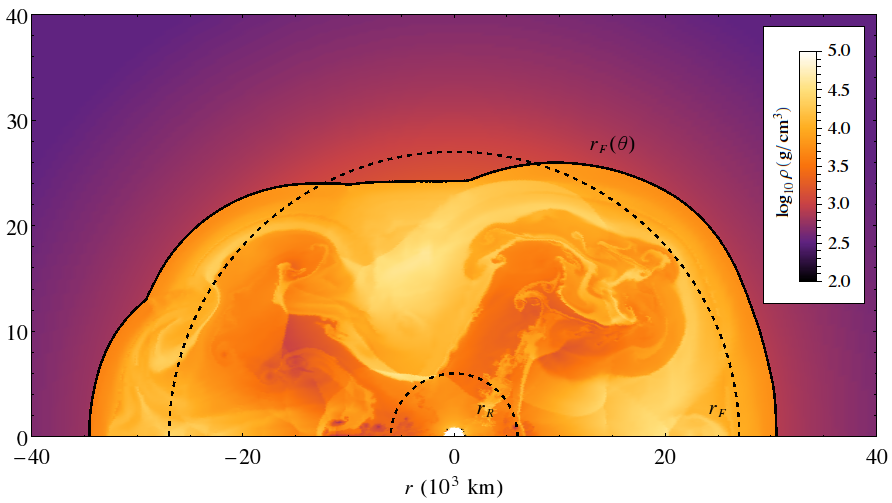
\includegraphics[height=0.5\textheight]{assets/supernova-shock-turbulence.png}
    \caption*{Supernova shock and turbulence. E. Borriello, et al  (2014)}
    %https://inspirehep.net/record/1262293?ln=en
    % arXiv: 1310.7488
\end{figure}



\end{frame}










\begin{frame}{Stimulated Neutrino Flavor Conversions}







\begin{equation*}
    \lambda(x) = \lambda_0\only<2>{ + A \cos(k x )}
\end{equation*}



\only<1>{
\begin{figure}
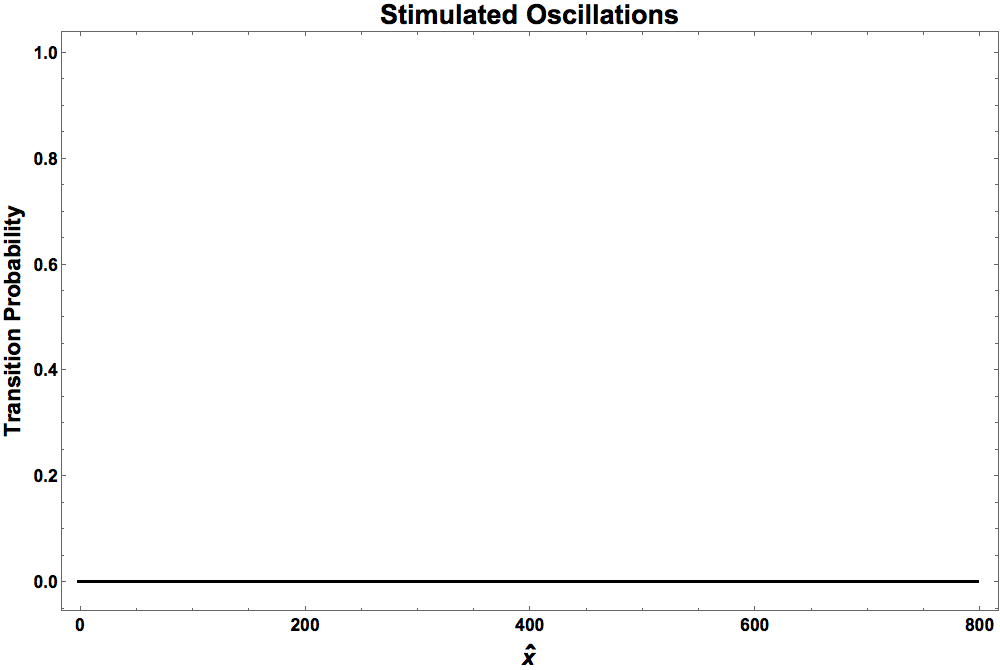
\includegraphics[width=0.8\textwidth]{assets/stimulated-oscillation-phenomenon-0.png}
\end{figure}
}




\only<2>{
\begin{figure}
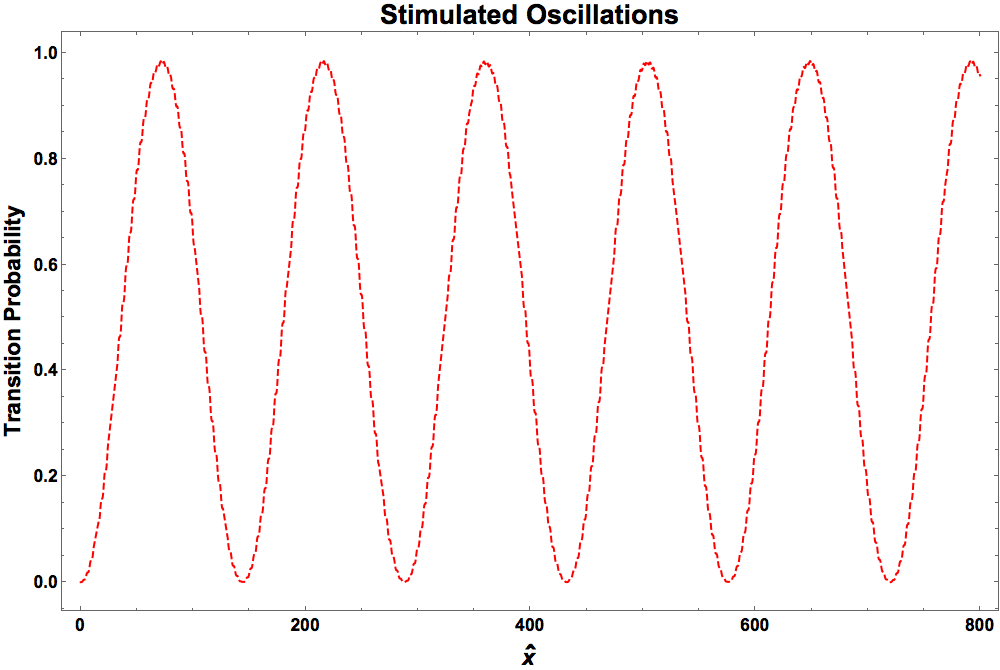
\includegraphics[width=0.8\textwidth]{assets/stimulated-oscillation-phenomenon.png}
%stimulated-neutrino-oscillations-kneller.png}
%\caption*{Stimulated oscillations. $\lambda(x) = \lambda_0 +  A \cos (k x)$
%with $\hat x = \omega_{\mathrm m} x $, $A=0.1\omega_{\mathrm m}$, $k=0.995\omega_{\mathrm m}$, $\theta_{\mathrm{m}}=\pi/6$
%}
\end{figure}
}


\only<1>{
\centering
Transition probabilities between mass states in matter.
}

\only<2>{
{\small
P. Krastev and A. Smirnov (1989); A. Friedland et al (2006); J. Kneller et al (2013); K. Patton et al (2014);
}
}


\end{frame}












%%%%%%%%%%%%%%%%%%%%%%%%%%%%%%%%
% Intuitive Demonstration BEGIN
%%%%%%%%%%%%%%%%%%%%%%%%%%%%%%%%







\begin{frame}{Rabi Oscillations}
\setbeamercovered{invisible}




\only<1,5>{

\begin{columns}[T]
\begin{column}{0.4\textwidth}
\begin{tcolorbox}[title=Rabi Oscillation]

Hamiltonian

\begin{equation*}
    -\frac{\omega_{\mathrm m}}{2} \sigma_3 - \frac{\alpha}{2} \begin{pmatrix}
    0 & e^{ikt}\\
    e^{-ikt} & 0
    \end{pmatrix}
\end{equation*}
\end{tcolorbox}

\end{column}%
\begin{column}{0.6\textwidth}
   \begin{tcolorbox}[title=Scheme]
\begin{figure}
    \centering
    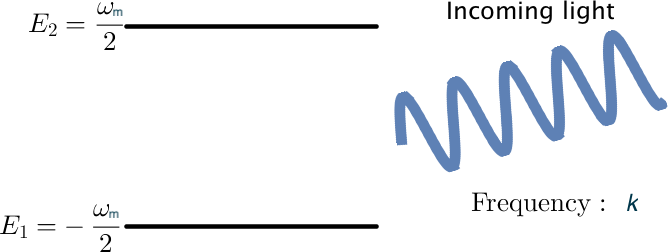
\includegraphics[width=\textwidth]{assets/rabi-diagram.png}
\end{figure}
\end{tcolorbox}


\end{column}
\end{columns}



}


\only<2-3>{



\begin{columns}[T]
\begin{column}<2-3>{0.5\textwidth}

\centering
Static Frame

\begin{equation*}
    \vec H_3 = \omega_{\mathrm m}\begin{pmatrix}
    0 \\
    0\\
    1
    \end{pmatrix}, \vec H_+ = \alpha  \begin{pmatrix}
    \cos( kt) \\
    -\sin(kt)\\
    0
    \end{pmatrix}
\end{equation*}

\begin{figure}
    \centering
    \includegraphics[width=0.8\textwidth]{assets/rabi-isospin-static-frame}
\end{figure}


\end{column}%
\begin{column}<3>{0.5\textwidth}

\centering
Corotating Frame

\begin{equation*}
    \vec H'_3 = (\omega_{\mathrm m} - k)\begin{pmatrix}
    0 \\
    0\\
    1
    \end{pmatrix}, \vec H'_+ = \alpha  \begin{pmatrix}
    1 \\
    0\\
    0
    \end{pmatrix}
\end{equation*}

\begin{figure}
    \centering
    \includegraphics[width=0.8\textwidth]{assets/rabi-isospin-rotating-frame}
\end{figure}





\end{column}
\end{columns}


}




\only<4>{

\centering
Corotating Frame


\begin{equation*}
    \vec H'_3 = (\omega_{\mathrm m} - k)\begin{pmatrix}
    0 \\
    0\\
    1
    \end{pmatrix} = 0 \Rightarrow k=\omega_{\mathrm m}
\end{equation*}


\begin{figure}
    \centering
    \includegraphics[width=0.5\textwidth]{assets/rabi-isospin-rotating-frame-resonance}
\end{figure}


}



\only<5>{



Rabi formula

\begin{equation*}
    P_{1\to 2} = \frac{1}{1 + D^2} \sin^2 \left( \frac{\Omega_{\mathrm R}}{2} t \right).
\end{equation*}

Relative detuning

\begin{equation*}
    D = \left\vert\frac{\omega_{\mathrm m} - k}{\alpha} \right\vert.
\end{equation*}

Rabi frequency

\begin{equation*}
\Omega_{\mathrm R} = \lvert\alpha\rvert\sqrt{1+ D^2}
\end{equation*}



}


\end{frame}



\begin{frame}{Hamiltonian in Matter Basis}

\begin{textblock*}{10pt}(220pt,1pt)
\small
\begin{equation*}
\begin{pmatrix}
\psi_e\\
\psi_\mu
\end{pmatrix} = \begin{pmatrix}
\cos \theta_m & \sin\theta_m \\
-\sin \theta_m & \cos \theta_m
\end{pmatrix}\begin{pmatrix}
\psi_L\\
\psi_H
\end{pmatrix}
\end{equation*}

\end{textblock*}


% Matter profile
\begin{tcolorbox}[title=Matter Potential]
\begin{equation*}
    \lambda(x)  = \lambda_0 \only<2>{ + {\color{red}A\cos(k x)} }
\end{equation*}
\end{tcolorbox}


% Basis


\begin{tcolorbox}[title=Basis]

\only<2>{Background} matter basis:


\begin{equation*}
    \mathbf H = \frac{1}{2}\left( - \omega_{\mathrm{m}}
    \only<2>{
    + {\color{red}A\cos(kx)} \cos 2\theta_{\mathrm{m}}
    }
    \right) \boldsymbol{\sigma_3}
    \only<2>{
    - \frac{{\color{red}A\cos(kx) } }{2} \sin 2\theta_{\mathrm{m}} \boldsymbol{\sigma_1}
    }
\end{equation*}


\end{tcolorbox}






\end{frame}






\begin{frame}{Hamiltonian in Matter Basis}

% \begin{textblock*}{10pt}(240pt,1pt)
% \small
% \begin{equation*}
% \alpha = \frac{\sin2\theta_{\mathrm m}}{2}A
% \end{equation*}

% \end{textblock*}


Matter potential frequency

\begin{equation*}
    k\sim \omega_{\mathrm m}
\end{equation*}


\begin{align*}
    \mathbf {H} =\,& \frac{1}{2}\left( - \omega_{\mathrm{m}}
    +\cancel{
     \cos 2\theta_{\mathrm{m}}{\color{red}A\cos(kx)} } \right) \sigma_3 - \frac{  \sin 2\theta_{\mathrm{m}
    }
    }{2}{\color{red}A \cos(kx)}  \sigma_1 \\
    \to\, &  \omega_{\mathrm m}\begin{pmatrix}
    0\\
    0\\
    1
    \end{pmatrix} + \alpha \begin{pmatrix}
    \cos (kx)\\
    -\sin(k x)\\
    0
    \end{pmatrix}  + \only<1>{\alpha \begin{pmatrix}
    \cos (-kx)\\
    -\sin( - k x)\\
    0
    \end{pmatrix}
    }
    \only<2>{\cancel{\alpha \begin{pmatrix}
    \cos (-kx)\\
    -\sin( - k x)\\
    0
    \end{pmatrix}
    }
    }
\end{align*}

\begin{equation*}
\alpha = \frac{\sin2\theta_{\mathrm m}}{2}A
\end{equation*}







\end{frame}



\begin{frame}{Rabi Formula Works}


% \begin{textblock*}{10pt}(230pt,-1pt)
% {\tiny
% \begin{equation*}
% \vec H \sim  \omega_{\mathrm m}\begin{pmatrix}
%     0\\
%     0\\
%     1
%     \end{pmatrix} + \alpha \begin{pmatrix}
%     \cos (kx)\\
%     -\sin(k x)\\
%     0
%     \end{pmatrix}
% \end{equation*}
% }
% \end{textblock*}

\begin{tcolorbox}
\begin{figure}
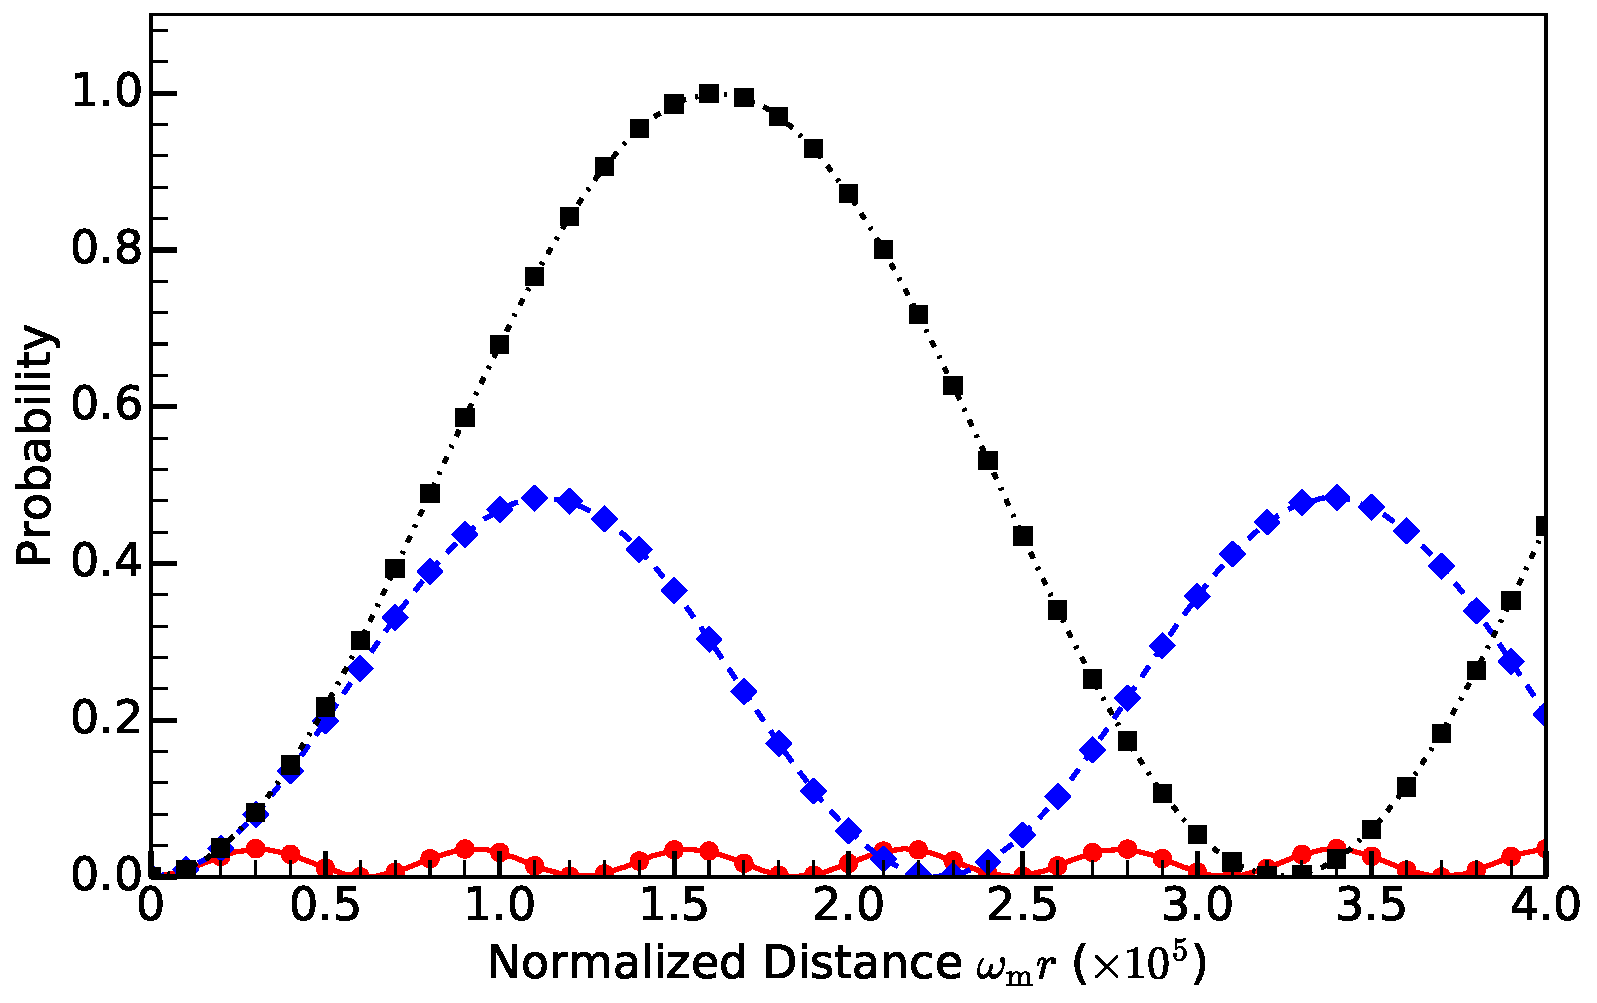
\includegraphics[width=0.9\textwidth]{assets/rabiOscillationsNeutrinoCoincidence-single-frequency}
%stimulated-neutrino-oscillations-kneller.png}
\caption*{
\color{black}Transition between two mass states in background matter potential $\lambda_0$\\
Lines: Rabi formula\\
Dots, diamonds, triangles, and squares are {\bf full solutions without approximations} for {\color{black}$k=\omega_{\mathrm m}$}, {\color{blue}$k=(1-2\times 10^{-5})\omega_{\mathrm m}$}, and {\color{red}$k=(1-10^{-4})\omega_{\mathrm m}$} respectively.
}
\end{figure}
\end{tcolorbox}

\end{frame}





\begin{frame}{Single Frequency Matter Potential Revisited}

We have been making approximations.


\begin{align*}
    \mathbf {H} =\,& \frac{1}{2}\left( - \omega_{\mathrm{m}}
    +\cancel{
     \cos 2\theta_{\mathrm{m}}{\color{red}A\cos(kx)} } \right) \sigma_3 - \frac{  \sin 2\theta_{\mathrm{m}
    }
    }{2}{\color{red}A \cos(kx)}  \sigma_1 \\
    \to\, &  \omega_{\mathrm m}\begin{pmatrix}
    0\\
    0\\
    1
    \end{pmatrix} + \alpha \begin{pmatrix}
    \cos (kx)\\
    -\sin(k x)\\
    0
    \end{pmatrix}  + \cancel{\alpha \begin{pmatrix}
    \cos (-kx)\\
    -\sin( - k x)\\
    0
    \end{pmatrix}
    }
\end{align*}


\end{frame}



\subsection{Basis and Formalism}



\begin{frame}{Rabi Basis}



\begin{tcolorbox}[title=Hamiltonian in Background Matter Basis]
    \begin{equation*}
    \mathbf {H} = \frac{1}{2}\left( - \omega_{\mathrm{m}} + {\color{red}A\cos(kx)} \cos 2\theta_{\mathrm{m}} \right) \boldsymbol{\sigma_3} - \frac{  {\color{red}A\cos (kx)}  }{2} \sin \theta_{\mathrm{m}} \boldsymbol{\sigma_1}.
\end{equation*}
\end{tcolorbox}


\begin{tcolorbox}[title=A Better Basis]


Define Rabi basis %\{$\ket{\tilde\nu_{\mathrm{L} }}$,$\ket{\tilde\nu_{\mathrm{H} }}$\}
in which the wave function is related to wave function in background matter basis
%\{$\ket{\nu_{\mathrm{L} }}$,$\ket{\nu_{\mathrm{H} }}$\}
through

\begin{equation*}
    \begin{pmatrix}
    \psi_{\mathrm{L} } \\
    \psi_{\mathrm{H} }
    \end{pmatrix} = \begin{pmatrix}
     e^{-i \eta (x)} & 0 \\  0 & e^{i \eta (x)}
    \end{pmatrix}\begin{pmatrix}
    \tilde\psi_{\mathrm{L} }\\
    \tilde\psi_{\mathrm{H} }
    \end{pmatrix},
\end{equation*}

where

\begin{equation*}
    \eta(x) - \eta(0) = \frac{\cos 2\theta_{\mathrm{m}}}{2} \int_0^x {\color{red}A\cos(k \tau)} d\tau.
\end{equation*}

\end{tcolorbox}



\end{frame}














\begin{frame}{Single Frequency Matter Potential}
% \setbeamercovered{invisible}



\begin{equation*}
\lambda(x) = \lambda_0 +  A \cos(k x )
\end{equation*}


\begin{tcolorbox}[title=Hamiltonian in Rabi Basis]

The Hamiltonian


\begin{equation*}
\mathbf{\widetilde H}= -\frac{\omega_{\mathrm m}}{2}\sigma_3 + \sum_{n=-\infty}^{\infty} \begin{pmatrix}
0 & \frac{1}{2}  \alpha_n e^{i  {\color{red} (n k) } x}\\
\frac{1}{2}  \alpha_n^* e^{ -i  {\color{red} (n k) } x} & 0
\end{pmatrix}
\end{equation*}


where $\alpha_n =  - (-i)^n  n  k \tan 2\theta_{\mathrm{m}}  J_n ( A \cos 2\theta_{\mathrm{m}} / k )$.


\end{tcolorbox}





\pause

\begin{tcolorbox}
\centering
Map neutrino oscillations in single frequency matter potential to Rabi oscillations with many driving potentials.
\end{tcolorbox}


\begin{tcolorbox}
\centering
Resonance condition for each mode: $nk=\omega_{\mathrm m}$
\end{tcolorbox}




\end{frame}



\begin{frame}{Rabi Oscillations With Multiple Driving Frequencies}


\only<1>{
Consider Rabi oscillation with two driving frequencies $k_1=n_1 k$, $k_2=n_2 k$

\begin{equation*}
    \vec H = \begin{pmatrix}
    0\\
    0\\
    \omega_m
    \end{pmatrix} + \alpha_1\begin{pmatrix}
     \cos(k_1x)\\
    -\sin(k_1x)\\
    0
\end{pmatrix} + \colorbox{blue!50}{$\alpha_2\begin{pmatrix}
    \cos(k_2x)\\
    -\sin(k_2x)\\
    0
    \end{pmatrix}$}
\end{equation*}

Corotating frame of the second potential,



\begin{equation*}
    \vec H = \begin{pmatrix}
    0\\
    0\\
    \omega_m - k_2
    \end{pmatrix} + \alpha_1\begin{pmatrix}
     \cos(k_1-k_2x)\\
    -\sin(k_1-k_2x)\\
    0
\end{pmatrix} + \colorbox{blue!50}{$\alpha_2\begin{pmatrix}
    1\\
    0\\
    0
    \end{pmatrix}$}
\end{equation*}

}

\only<1>{
Energy gap in this frame becomes the length of the vector

\begin{equation*}
    \begin{pmatrix}
    0\\
    0\\
    \omega_m - k_2
\end{pmatrix} + \colorbox{blue!50}{$\alpha_2\begin{pmatrix}
    1\\
    0\\
    0
    \end{pmatrix}$}
\end{equation*}
}

\only<2->{

% Energy gap in this frame becomes the length of the vector
% \begin{equation*}
% \sqrt{(\omega_{\mathrm m} - k_2)^2 + \alpha_2^2 } \to \omega_{\mathrm m} - k_2 + \frac{1}{2}\frac{\alpha_2^2}{\omega_{\mathrm m}-k_2}
% \end{equation*}

Relative detuning

\begin{equation*}
D' =  \left\vert \frac{\omega_{\mathrm m} - k_1 }{\alpha_1} + \frac{\alpha_2^2}{2\alpha_1(\omega_{\mathrm m}-k_2)} \right\vert
\end{equation*}

}

\end{frame}


\begin{frame}{Rabi Oscillations With Multiple Driving Frequencies}

\begin{textblock*}{100pt}(260pt,10pt)
% \textblockcolour{black}
\tiny
\begin{equation*}
D' =  \left\vert \frac{\omega_{\mathrm m} - k_1 }{\alpha_1} + \frac{\alpha_2^2}{2\alpha_1(\omega_{\mathrm m}-k_2)} \right\vert
\end{equation*}
\end{textblock*}


\begin{figure}
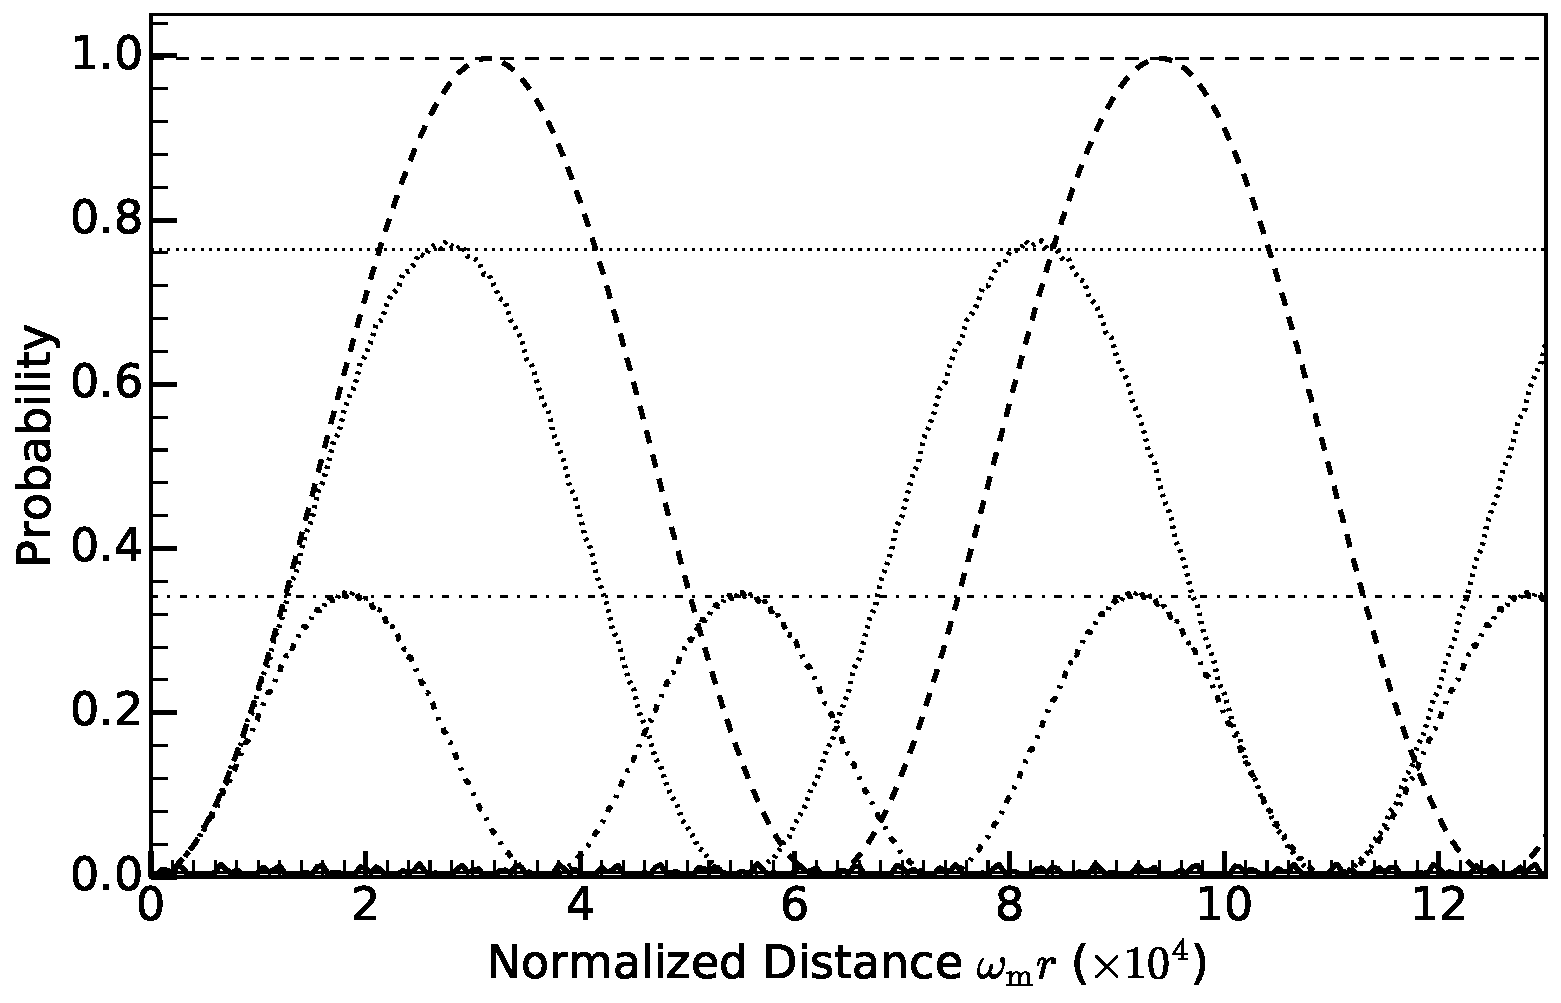
\includegraphics[width=0.9\textwidth]{assets/interference-reduction}
\caption*{Grid lines: amplitude predicted using $1/(1+D'^2)$
}
\end{figure}

% Dashed line, dotted line, dash-dotted line, and solid line are for $A_2=10^{-2}\omega_{\mathrm{m}}$, $k_2=10\omega_{\mathrm m}$, $A_2=10^{-2}\omega_{\mathrm{m}}$, $k_2=10^{-1}\omega_{\mathrm m}$, $A_2=5.0\times 10^{-2}\omega_{\mathrm{m}}$, $k_2=10\omega_{\mathrm m}$, and $A_2=5\times 10^{-2}\omega_{\mathrm{m}}$, $k_2=10^{-1}\omega_{\mathrm m}$

{\tiny
\vspace{-15pt}
\begin{center}
    \begin{tabular}{c|c|c|c}
    \multicolumn{4}{c}{ $\alpha_2$, $k_1$ values} \\
    \hline
       Dashed  &  dotted & dash-dotted & solid \\
       $10^{-2}\omega_{\mathrm{m}}$, $10\omega_{\mathrm m}$  &  $10^{-2}\omega_{\mathrm{m}}$, $10^{-1}\omega_{\mathrm m}$  & $5.0\times 10^{-2}\omega_{\mathrm{m}}$, $10\omega_{\mathrm m}$  & $5\times 10^{-2}\omega_{\mathrm{m}}$, $10^{-1}\omega_{\mathrm m}$
    \end{tabular}
\end{center}
}

\end{frame}



\begin{frame}{Rabi Oscillations With Multiple Driving Frequencies}



Consider $k_1=\omega_{\mathrm m}$

\begin{equation*}
D' =  \left\vert \frac{\alpha_2^2}{2\alpha_1(\omega_{\mathrm m}-k_2)} \right\vert
\end{equation*}

Amplitude reduces from 1 to 1/2 if

\begin{equation*}
    D'=1 \Rightarrow \alpha_{2,\mathrm C} \equiv \sqrt{ 2 \lvert \alpha_1 (k_2 - \omega_{\mathrm m}) \rvert }.
\end{equation*}


\vspace{2em}

\begin{tcolorbox}
Two driving frequencies $k_1$, and $k_2$, with amplitude $\alpha_1$, and $\alpha_2$

For $k_1 = \omega_{\mathrm m}$, survival of resonance requires

\begin{equation*}
    \lvert \alpha_2\rvert \ll  \alpha_{2,\mathrm C}\equiv\sqrt{ 2 \lvert \alpha_1 (k_2 - \omega_{\mathrm m}) \rvert }
\end{equation*}

\end{tcolorbox}






\end{frame}









\begin{frame}{Single Frequency Matter Potential}


\only<1->{

\begin{tcolorbox}
\begin{figure}
\centering
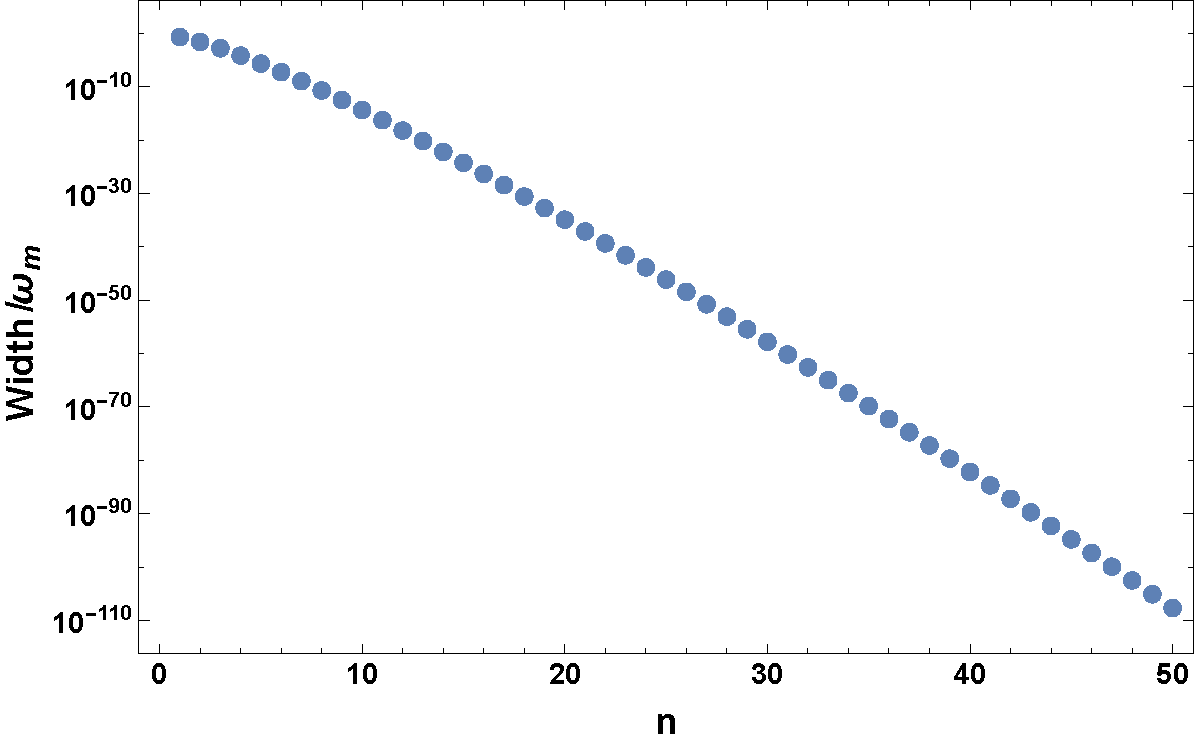
\includegraphics[width=0.95\textwidth]{assets/width-n}
\caption*{\color{black}Width of different modes given value of matter potential frequency $k$}
\end{figure}
\end{tcolorbox}
}

\only<2->{
\begin{textblock*}{280pt}(40pt,100pt)
\begin{tcolorbox}
   \centering
Higher modes are less important
\end{tcolorbox}
\end{textblock*}
}



\end{frame}



\begin{frame}<presentation:0>[noframenumbering]{Single Frequency Matter Potential}

Resonance conditions:

\begin{equation*}
    nk=\omega_{\mathrm m}
\end{equation*}

However, higher order resonances for n large usually have extremely small width.



\end{frame}



\subsection{Multiple Frequencies in Matter Potential}


\begin{frame}{Multiple Frequencies in Matter Potential}
\setbeamercovered{invisible}




\begin{equation*}
\lambda(x) = \lambda_0 + \sum_{a=1}^N A_a \sin(k_a x )
\end{equation*}


\begin{tcolorbox}[title=Hamiltonian in Rabi Basis]


\begin{equation*}
\mathbf{\widetilde H}= -\frac{\omega_{\mathrm m}}{2}\sigma_3 + \frac{1}{2} \sum_{n_1=-\infty}^\infty \cdots \sum_{n_N=-\infty}^\infty \begin{pmatrix}
0 &  B_{\{n_a\}} e^{i  {\color{red} \sum_a n_a k_a } x}\\
  B_{\{n_a\}}^* e^{ -i  {\color{red} \sum_a n_a k_a } x} & 0
\end{pmatrix}
\end{equation*}


where
\begin{align*}
    B_{\{n_a\}} &= -(-i)^{\sum_a n_a} \tan 2\theta_m \left( \sum_a n_a k_a \right) \left( \prod_a J_{n_a}\left( \frac{A_a}{k_a}\cos 2\theta_m \right) \right)
    %\Phi_{\{n_a\}} &= e^{i\left( \sum_a n_a \phi_a \right)}.
\end{align*}




\end{tcolorbox}




\end{frame}



\begin{frame}{Castle Wall Matter Potential}



\begin{columns}[T]
\begin{column}{0.5\textwidth}

\only<1,2>{

\begin{figure}
    \centering
    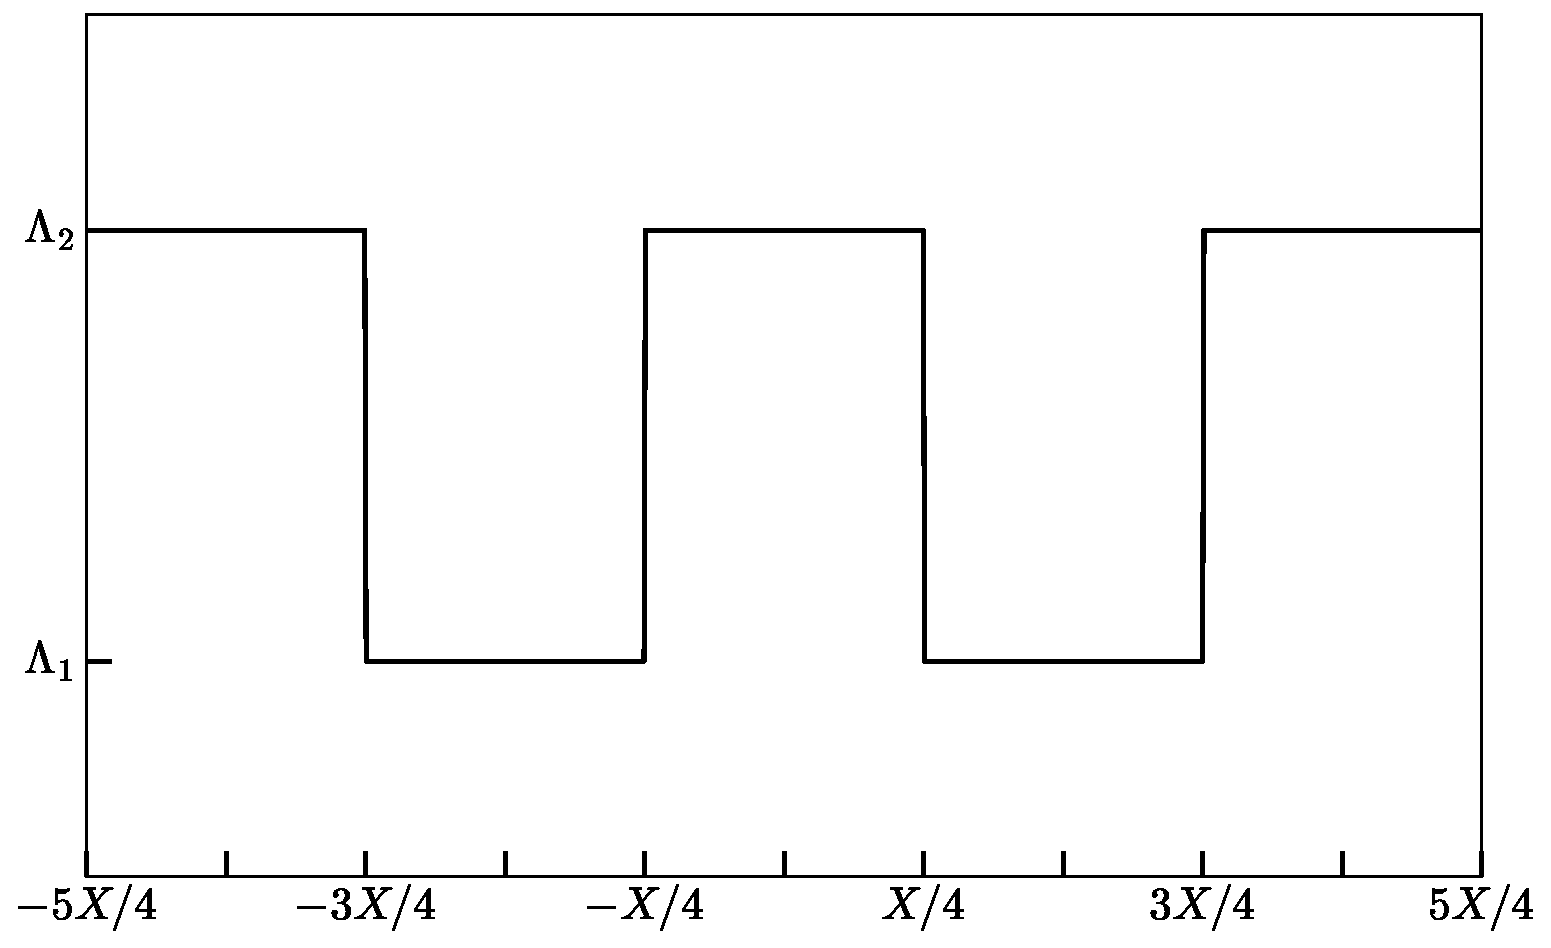
\includegraphics[width=\columnwidth]{assets/castlewall-profile}
    \caption*{Castle wall matter profile: $\Lambda_2 =0.35\omega_{\mathrm v} \cos 2\theta_{\mathrm v} $,  $\Lambda_1 = 0.15\omega_{\mathrm v} \cos 2\theta_{\mathrm v}$ and period $X =2\pi/\omega_{\mathrm m}$ }
\end{figure}

}

% \only<3>{
% \begin{table}
% \caption*{Relative detuning of each frequency.}
% \begin{tabular}{lll}
%  $\{n_1,n_2\}$  & $D'_{\{n_1,n_2\}}$   \\
% \hline \\
%  $\{1,0\}$ & $0$  \\
%  $\{1,0\}$ \& $\{-1,0\}$ &  $1.0\times 10^{-2}$ \\
%  $\{1,0\}$ \& $\{0,1\}$ &   $1.1\times 10^{-3}$  \\
%  $\{1,0\}$ \& $\{2,0\}$ &  $2.0\times 10^{-4}$
% \end{tabular}
% \end{table}

% }

\end{column}%
\begin{column}{0.5\textwidth}

\only<1>{
\small
\begin{equation*}
    \lambda(x)= \lambda_0 + \sum_1^\infty \lambda_n \cos (k_n x)
\end{equation*}

where

\begin{align*}
    \lambda_0 = & (\Lambda_1+\Lambda_2)/2 \\
    \lambda_n = & 2(-1)^n(\Lambda_1-\Lambda_2)/(2n\pi-\pi) \\
    k_n =& 2\pi (2n-1)/X
\end{align*}
}

\only<2>{
\begin{figure}
        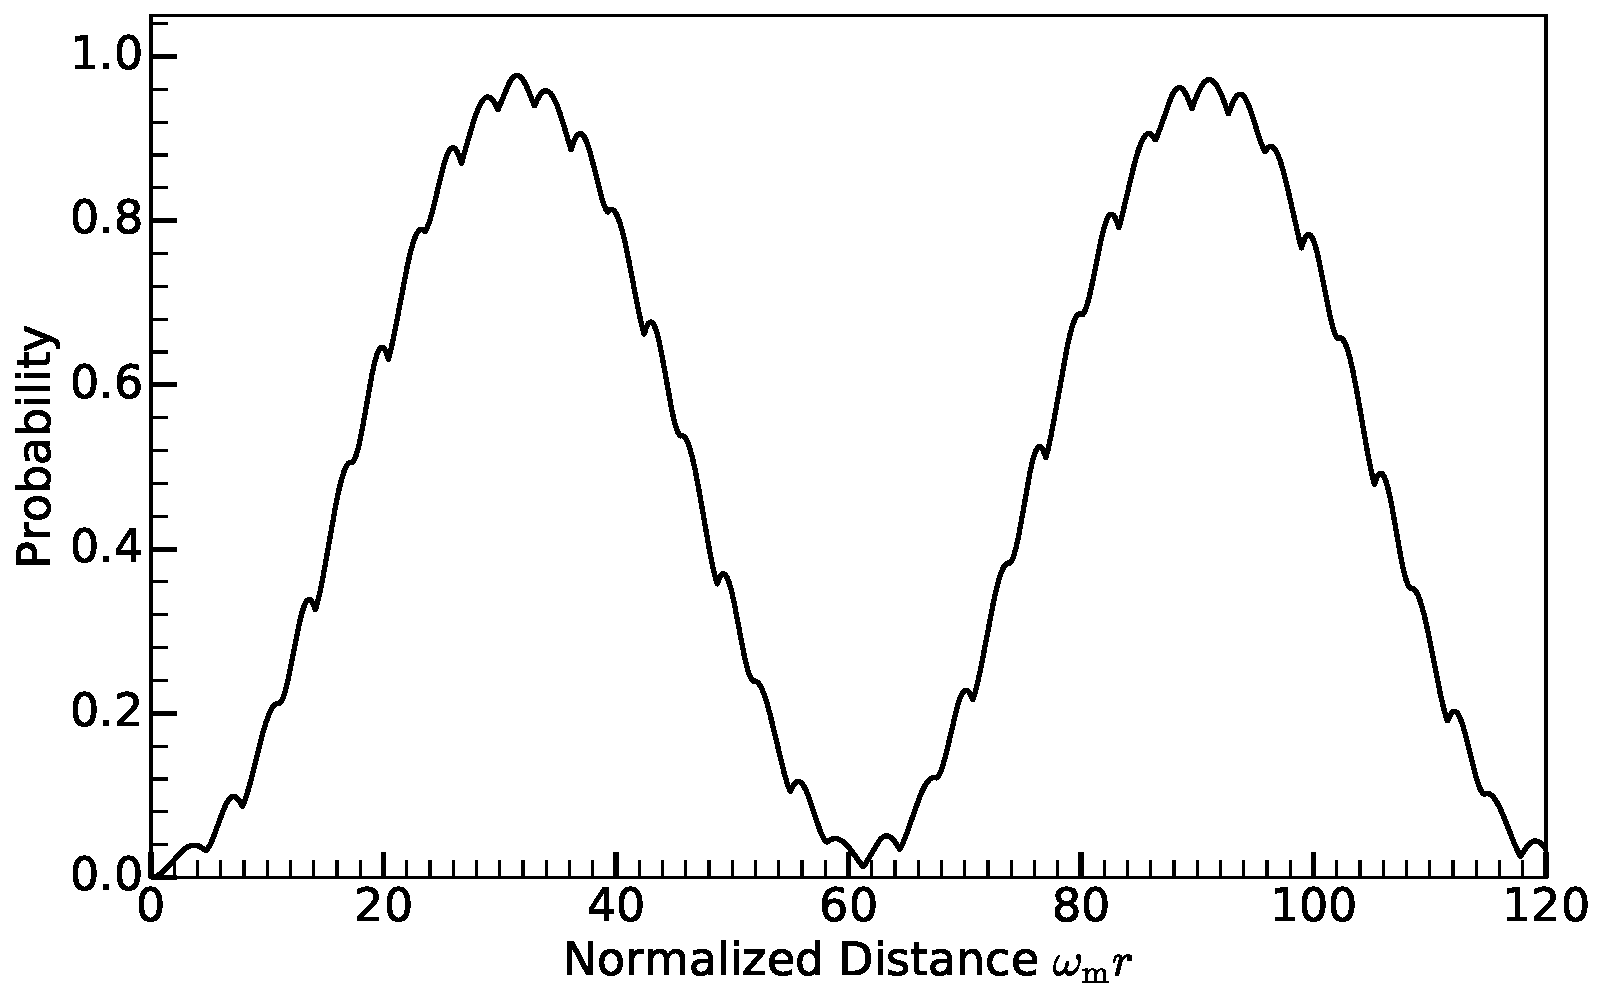
\includegraphics[width=\columnwidth]{assets/castle-wall-1}%
     \caption*{Transition probability is a Rabi resonance with small variations due to higher orders.}
\end{figure}
}

\end{column}
\end{columns}




\end{frame}



\begin{frame}{Summary of Stimulated Oscillations}


\begin{columns}[T]
\begin{column}{0.6\textwidth}

\begin{enumerate}[<+->]
\item
Vacuum oscillations: flavor sates are not mass states.
\item
MSW resonance: matter potential cancels out the vacuum diagonal elements of the Hamiltonian.
\item
Stimulated oscillations: variation in matter potential can cause resonances.

\item
In many cases neutrino oscillations in multi-frequency matter potential can be viewed as Rabi oscillations with few driving frequencies.
\end{enumerate}

\end{column}
\begin{column}{0.4\textwidth}

\only<1>{
\begin{figure}
    \centering
    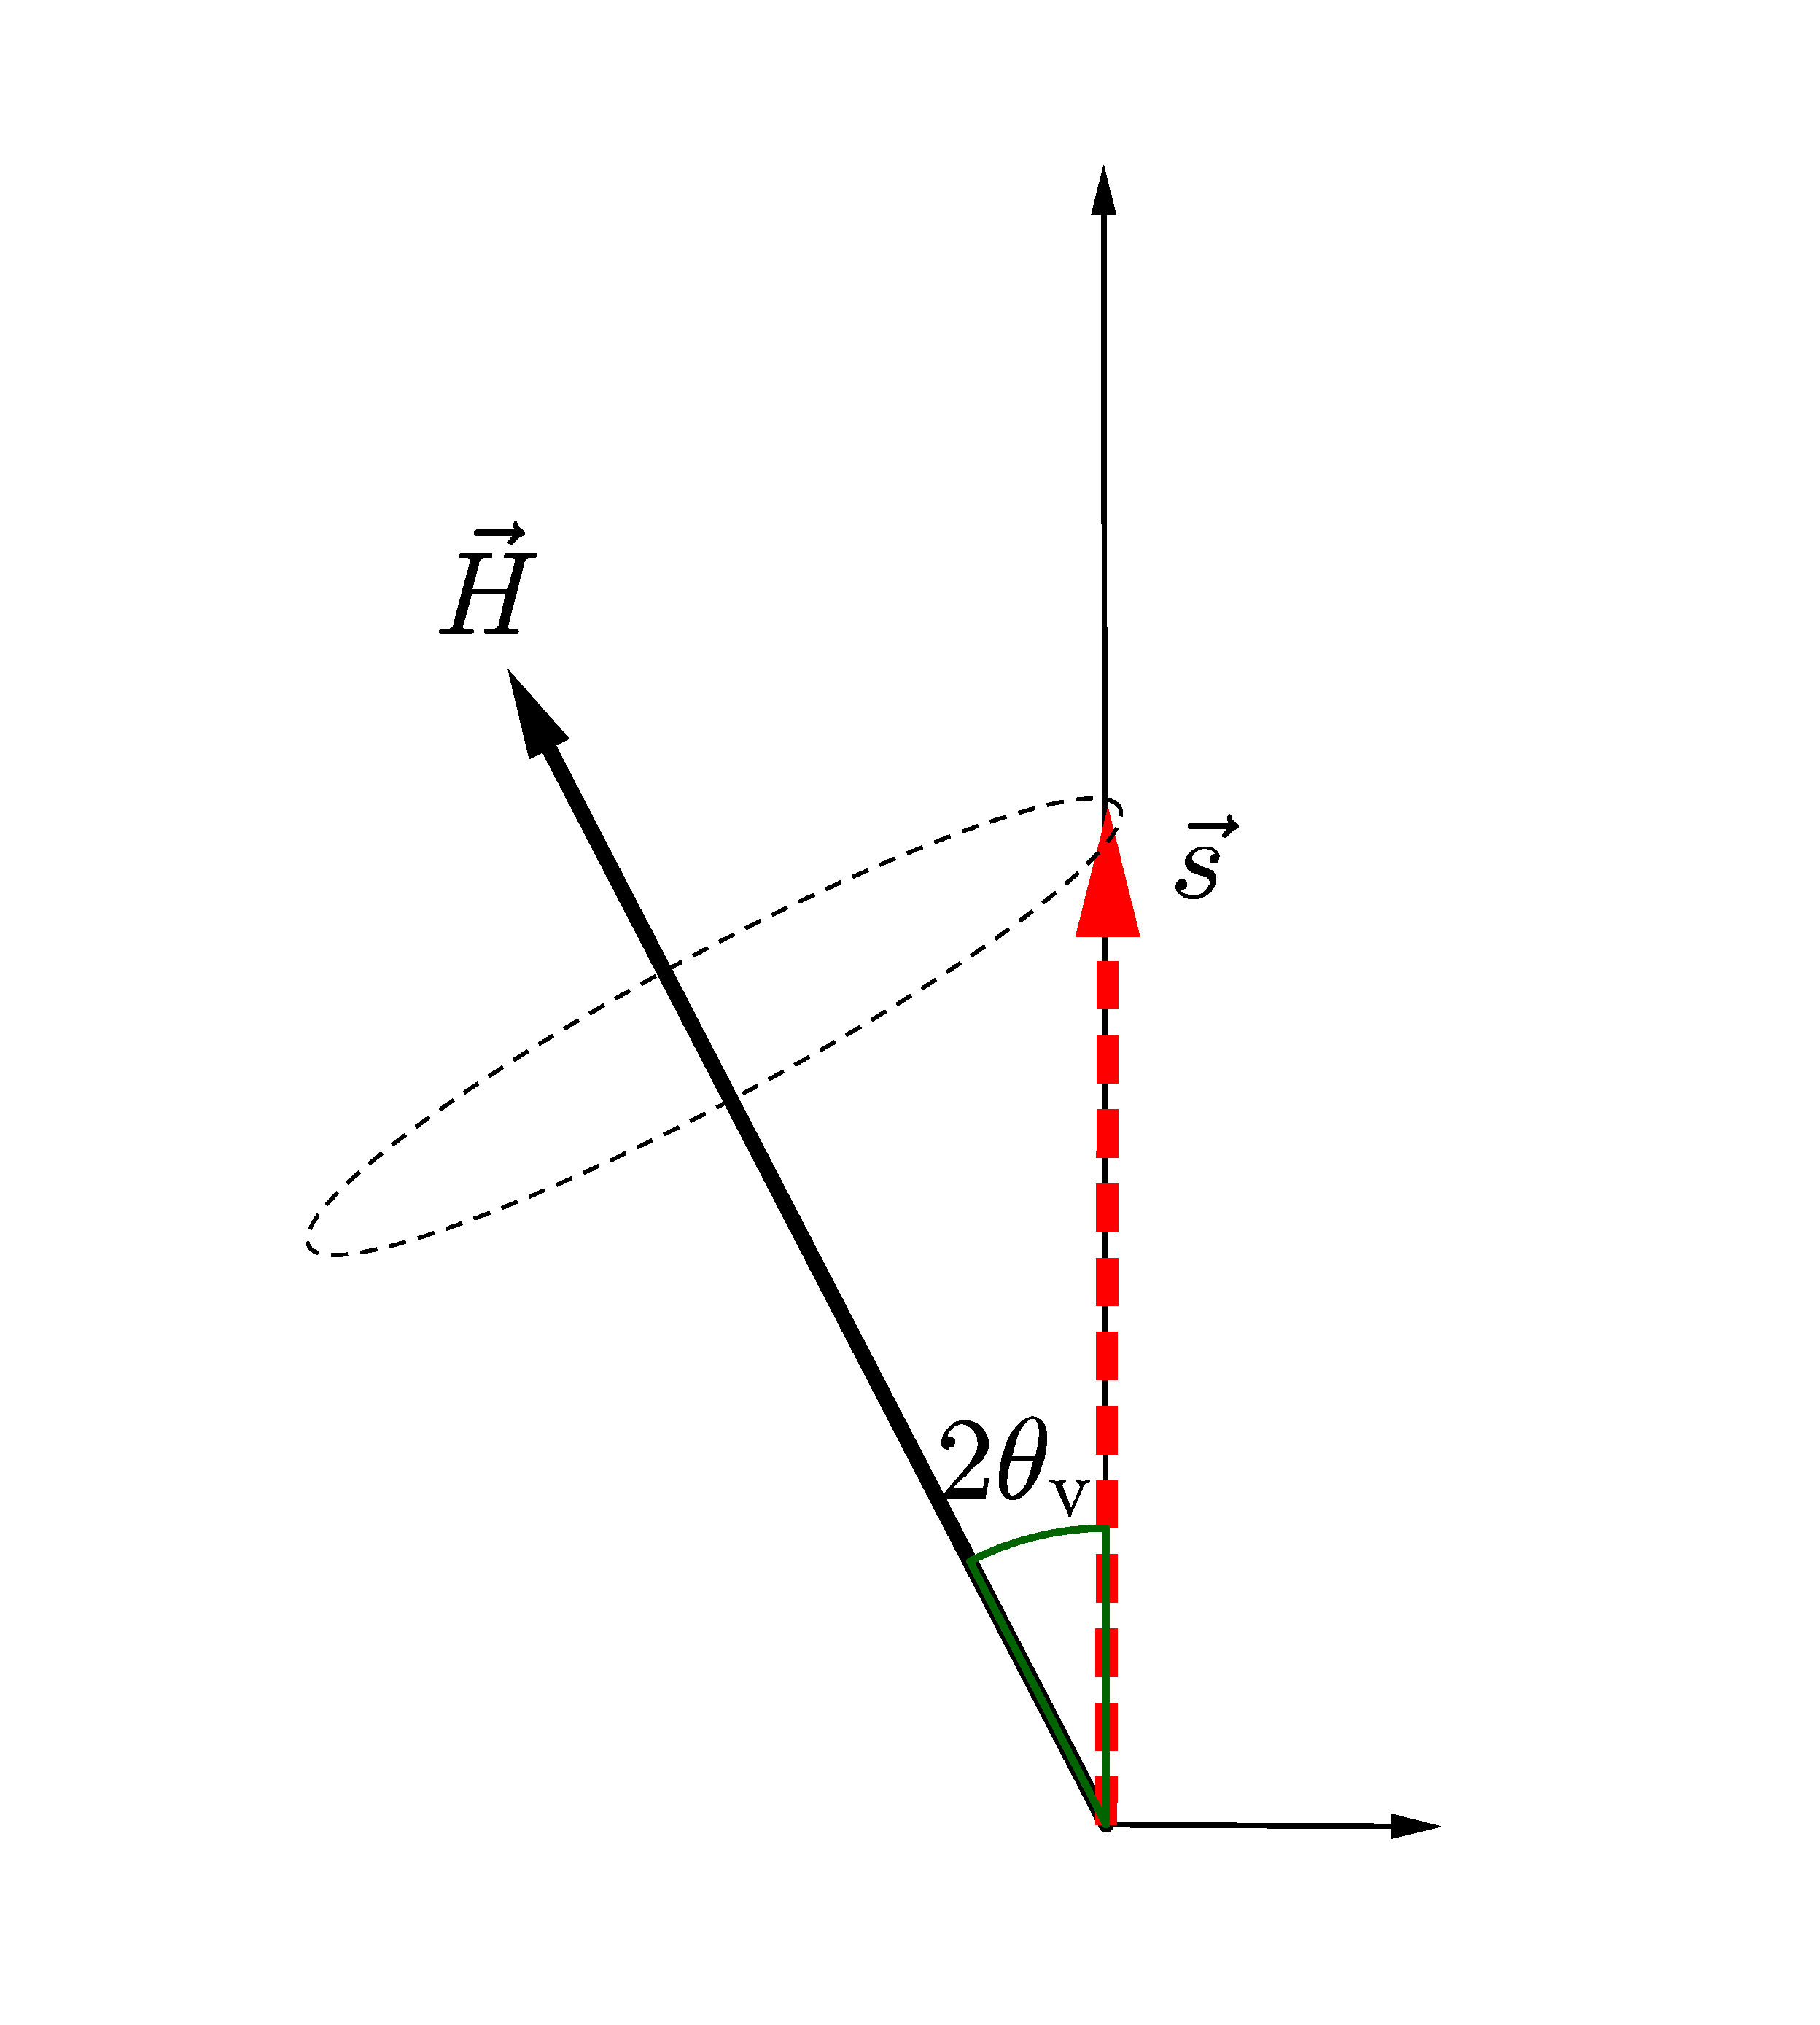
\includegraphics[width=0.9\textwidth]{assets/flavor-isospin-1}
\end{figure}
}

\only<2>{
\begin{figure}
    \centering
    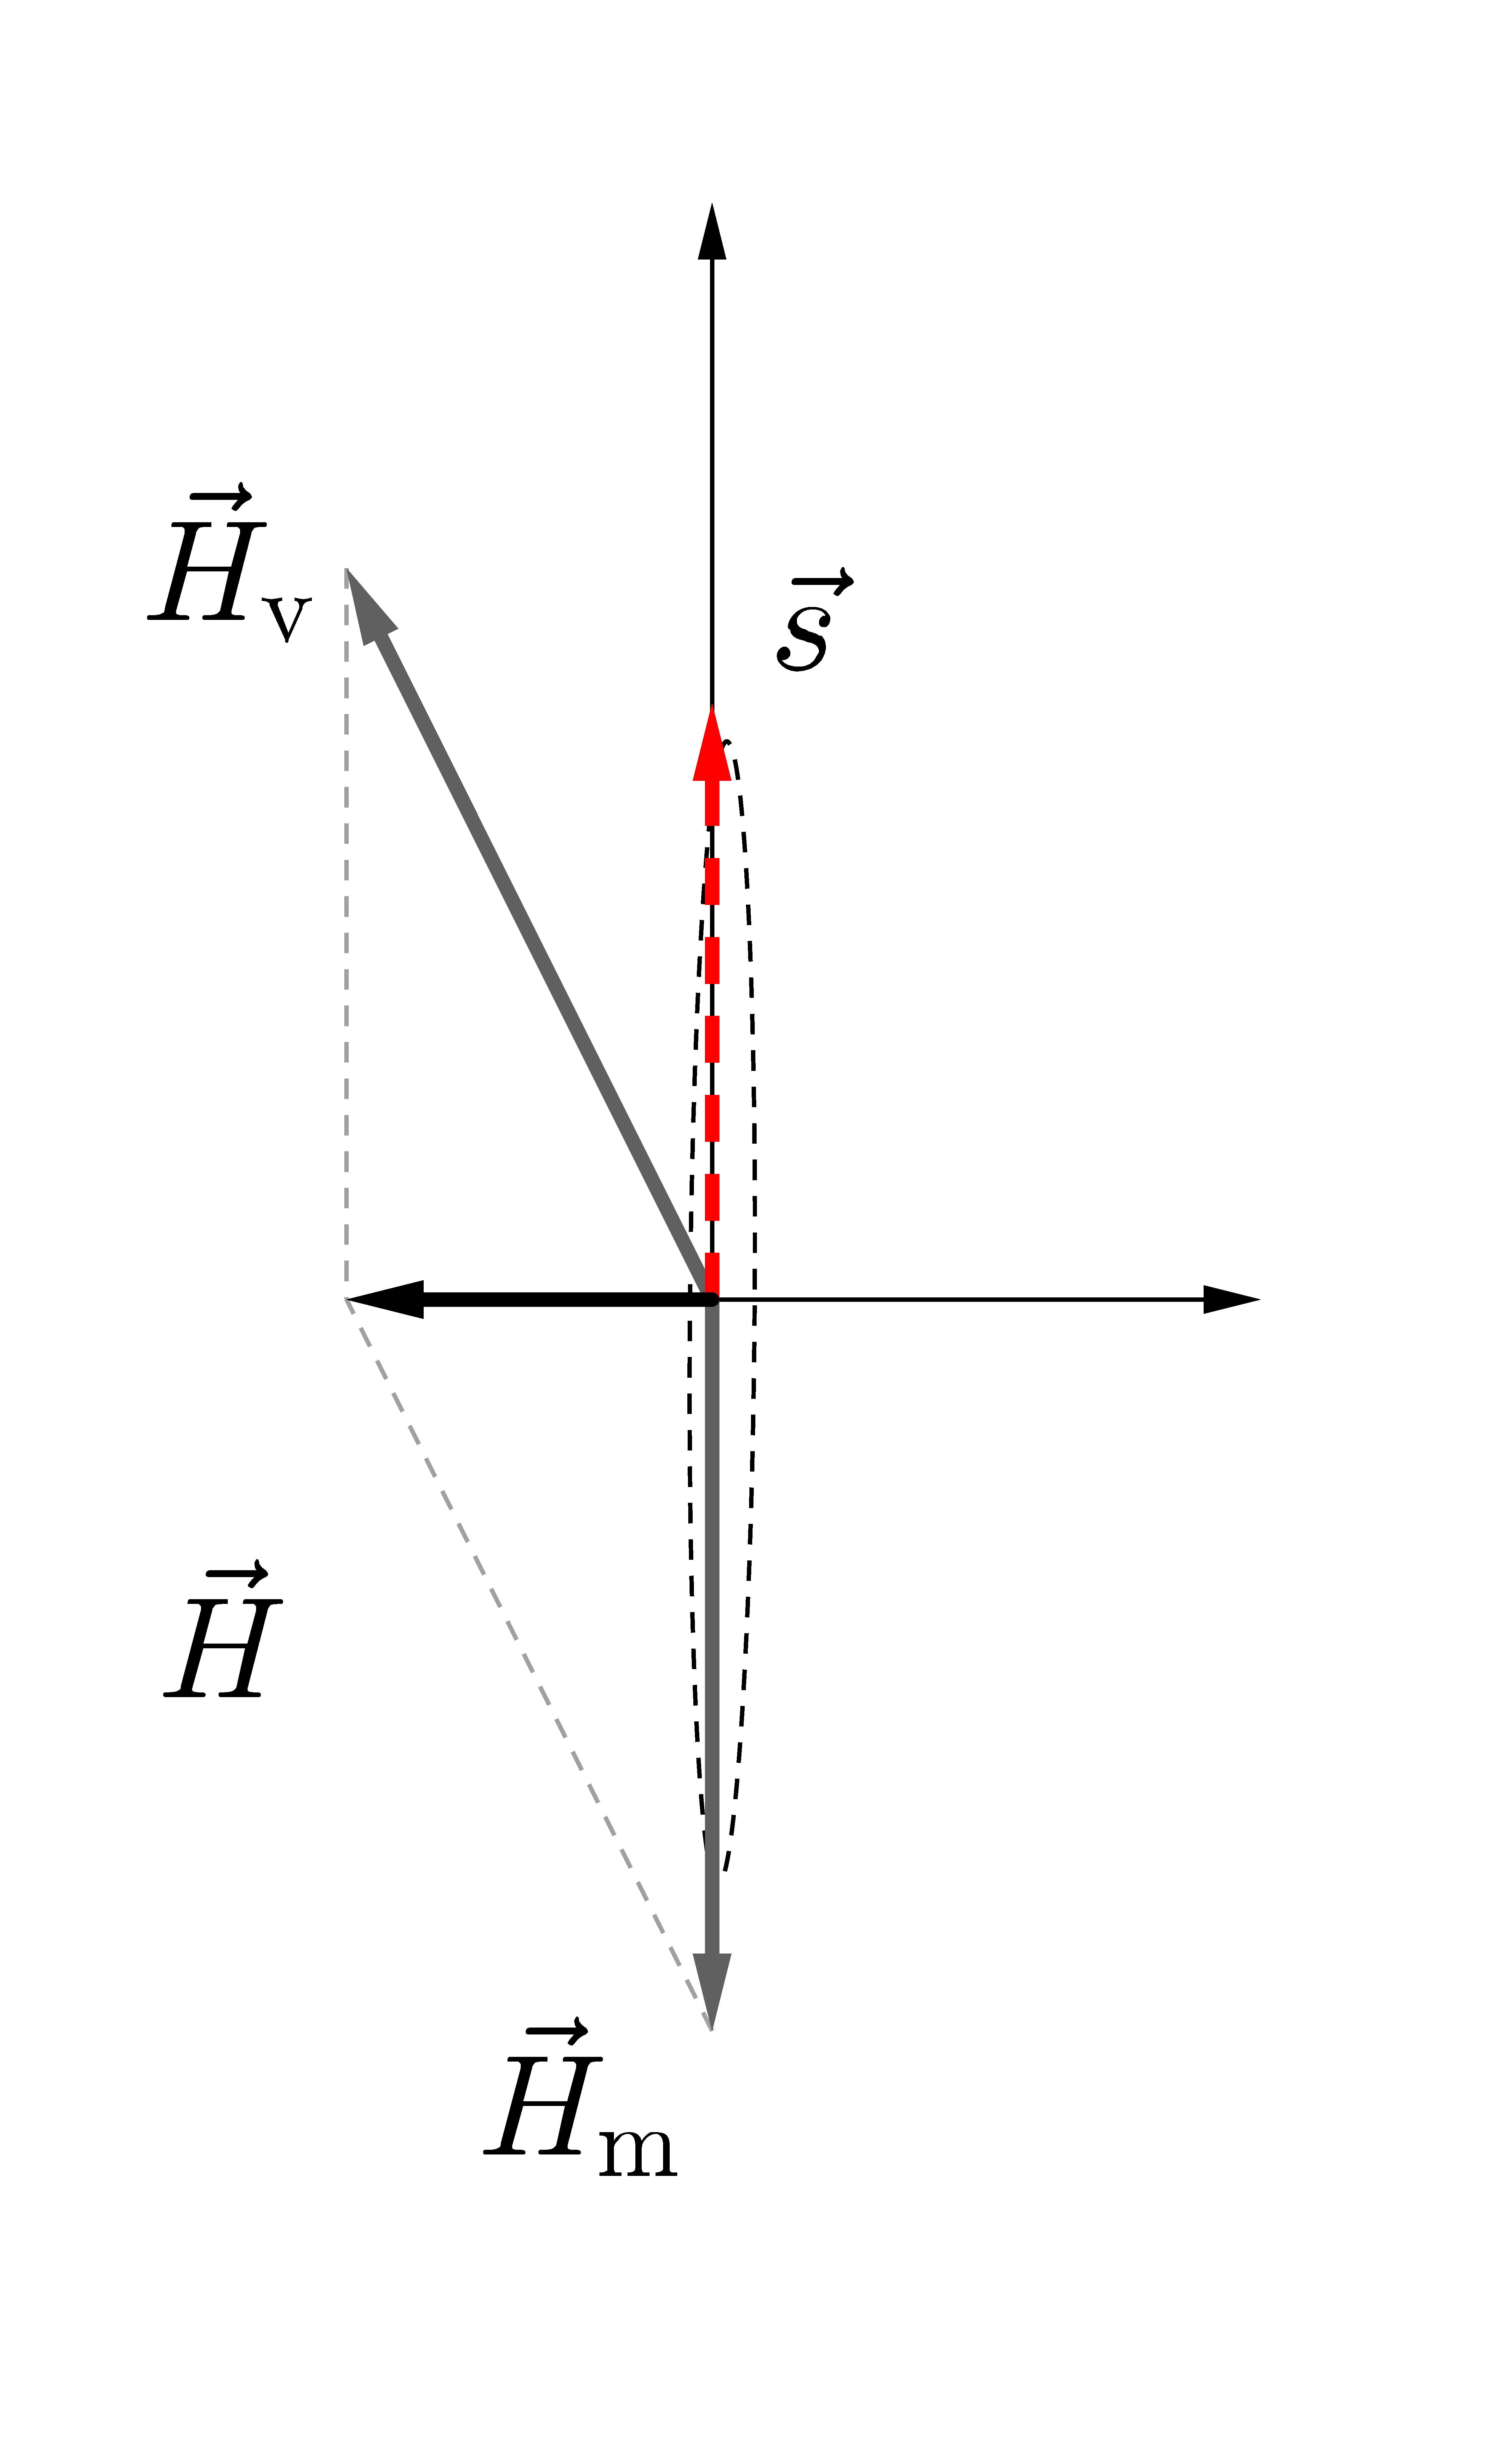
\includegraphics[width=0.9\textwidth]{assets/matter-effect-critical-density}
\end{figure}
}

\only<3>{
For matter potential

\begin{equation*}
\lambda(x) = \lambda_0 + A\cos(k x),
\end{equation*}

Resonance condition

\begin{equation*}
    n k = \omega_{\mathrm m}
\end{equation*}

}

\only<4>{


% \begin{equation*}
% \lvert \alpha_2\rvert \gg \alpha_{2,\mathrm C} \equiv \sqrt{ 2 \lvert \alpha_1 (k_2 - \omega_{\mathrm m}) \rvert }
% \end{equation*}


}

\end{column}
\end{columns}

\end{frame}



%%%%%%%%%%%%%%%%%%%%%%%%%%%%%%%%%%%%%%%%%%%%%%%%%%%%%%%%%
%%%%%%%%% Dispersion Relation




\section{Neutrino Oscillations and Dispersion Relation}

\subsection{Neutrino Self-interactions}

\begin{frame}{Neutrino Self-interactions}


\begin{columns}[T]
   \begin{column}{0.5\textwidth}

      Interaction Hamiltonian $\mathbf H_{\nu\nu}$

      \begin{equation*}
         \sqrt{2}G_{\mathrm F} (1- \hat p \cdot \hat p') \rho( \mathbf p' )
      \end{equation*}

      In Flavor Isospin space
      \begin{equation*}
         -2\sqrt{2}G_{\mathrm F} (1- \hat p \cdot \hat p') n(\mathbf p') \vec s ( \mathbf p' )
      \end{equation*}

      % \only<2>{
         % \begin{tcolorbox}
            % \begin{figure}
            %    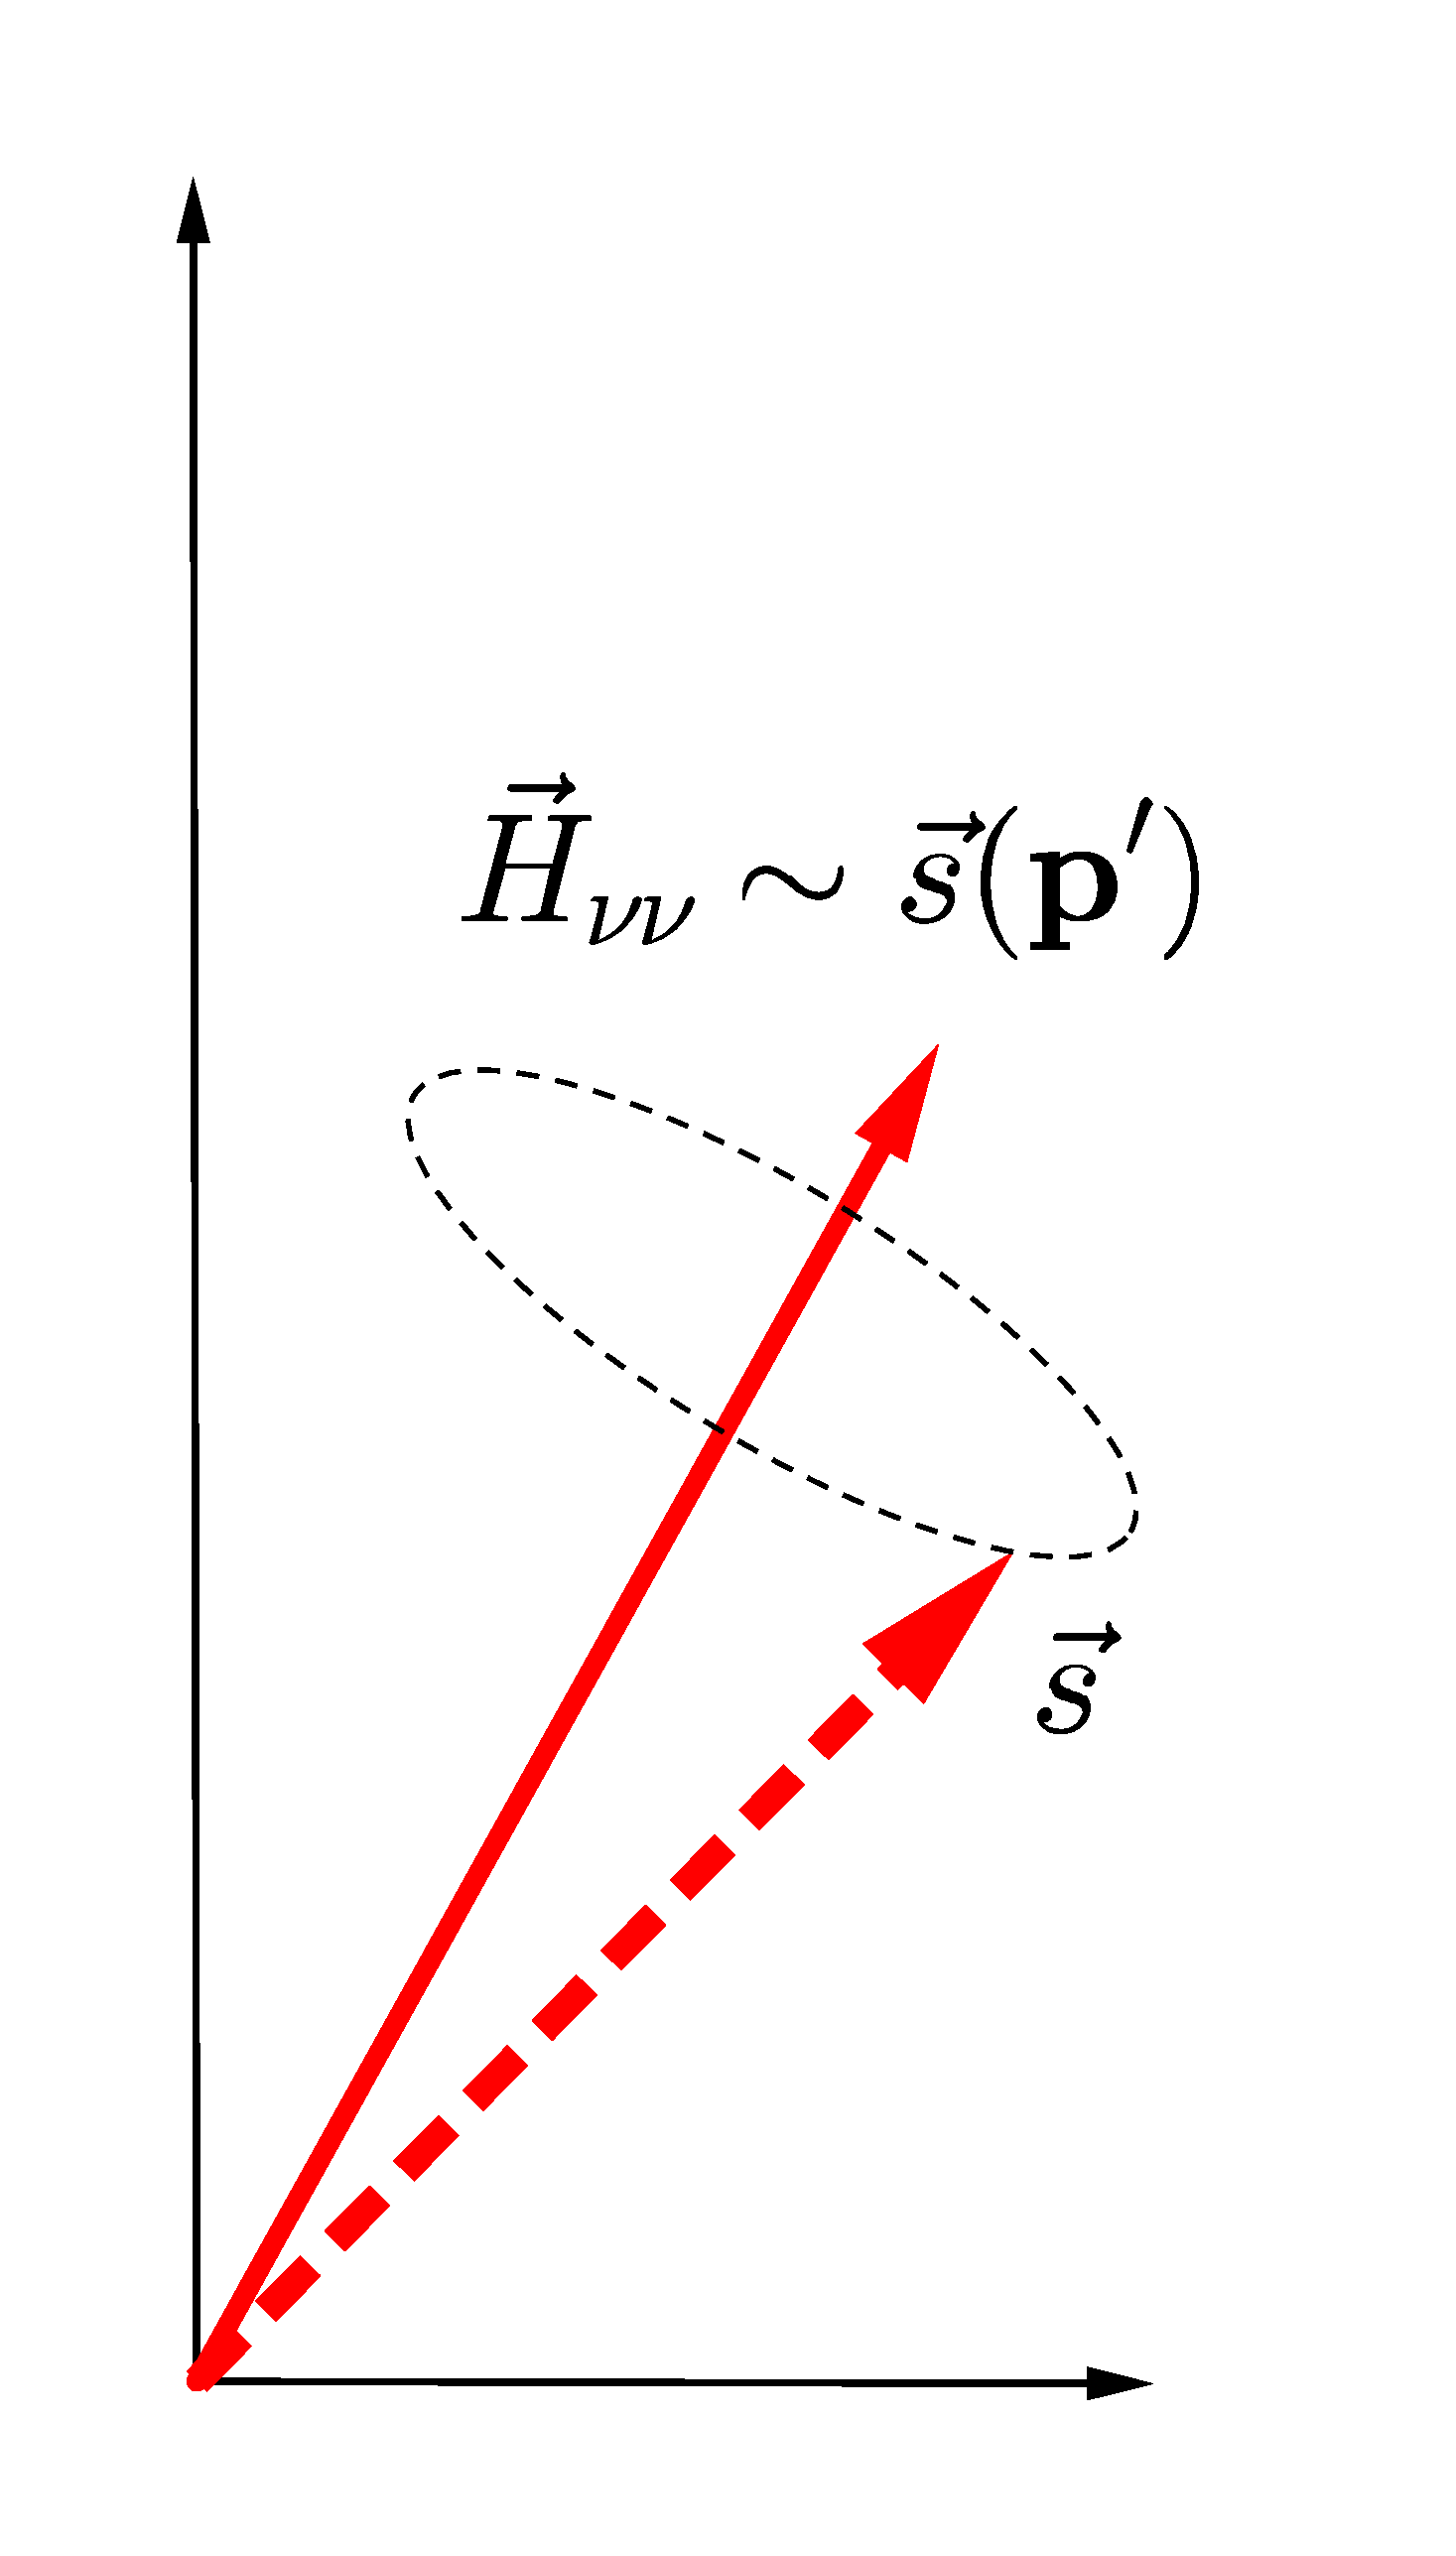
\includegraphics[width=\textwidth]{assets/self-interaction}
            % \end{figure}

         % \end{tcolorbox}
      % }


   \end{column}

   \begin{column}{0.5\textwidth}

      \begin{figure}
         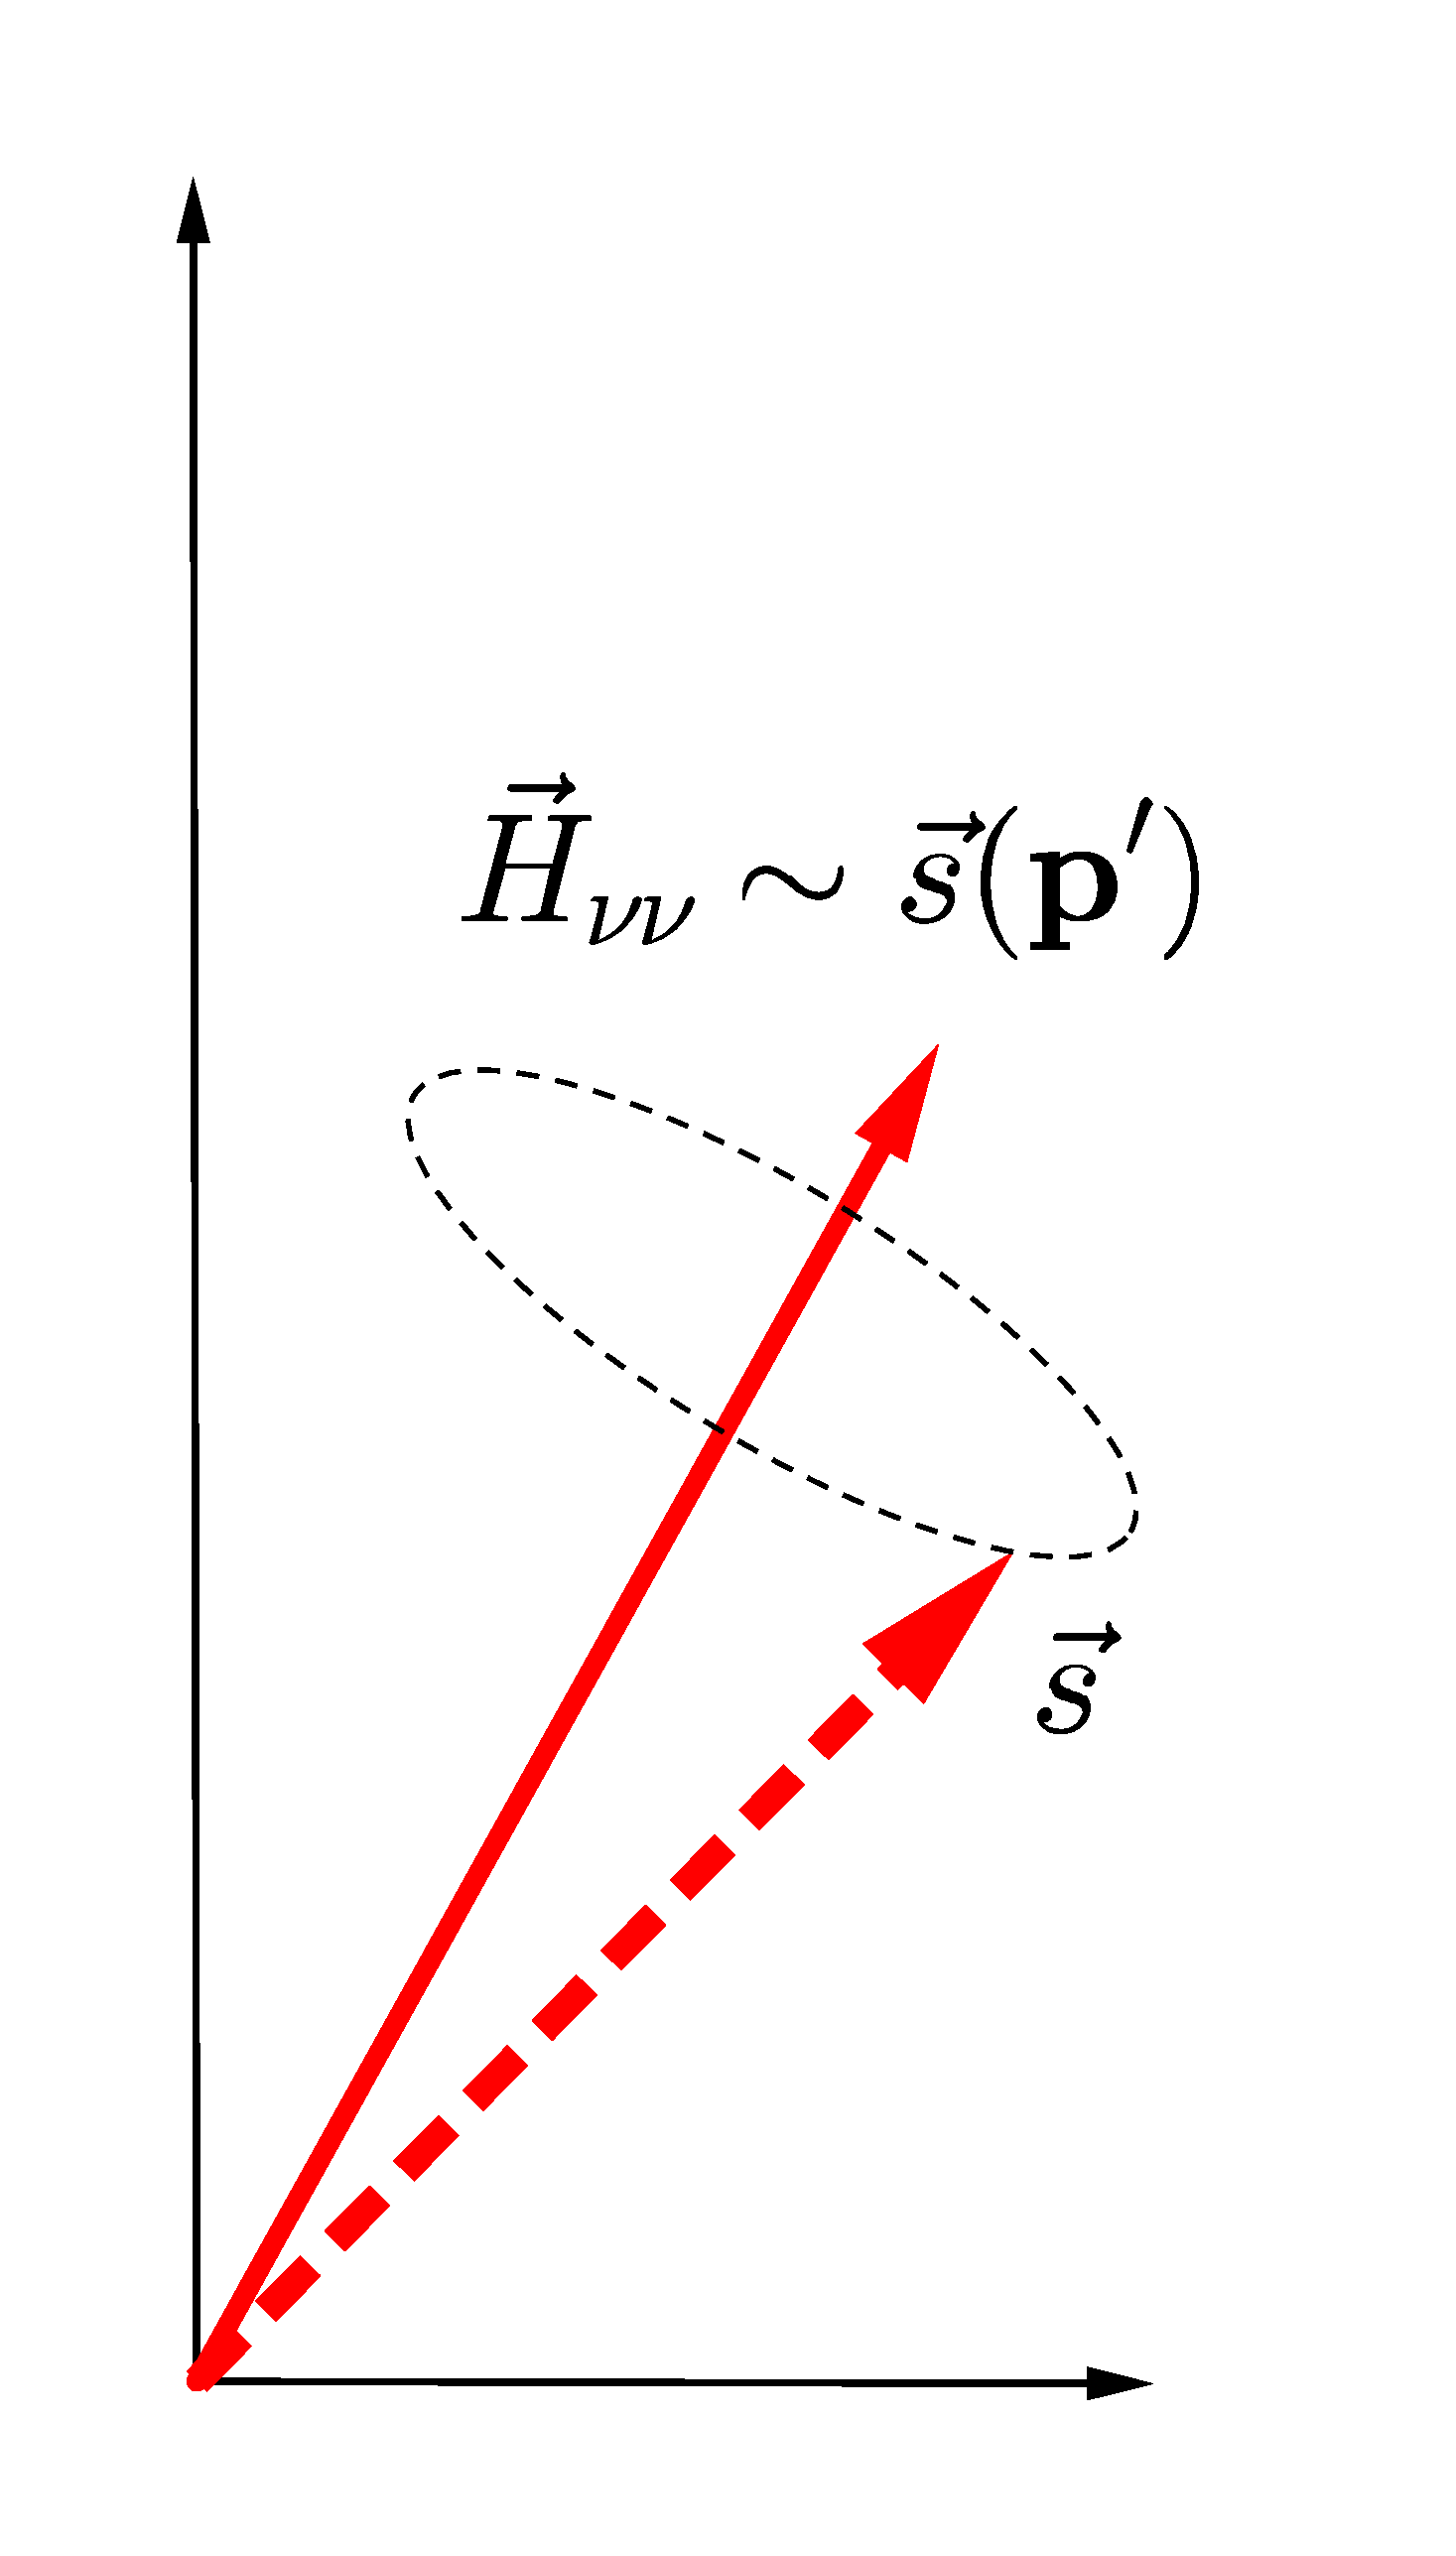
\includegraphics[width=0.8\textwidth]{assets/self-interaction}
      \end{figure}




   \end{column}


\end{columns}





\end{frame}

\begin{frame}{Neutrino Self-interactions}

\begin{columns}[T]

\begin{column}{0.3\textwidth}

\begin{itemize}
   \item $H_v = - \eta \frac{1}{2}\omega \sigma_3 $
   \item $H_m = \frac{1}{2}\lambda \sigma_3$
   \item $H_{\nu\nu,2} = \frac{1}{2}\mu_1 \rho_1 \xi $
   \item $H_{\nu\nu,1} = \frac{1}{2}\mu_2 \rho_2 \xi$
\end{itemize}
where
\begin{equation*}
   \mu_i = \sqrt{2} G_{\mathrm F} \xi n_i
\end{equation*}

Geometric factor
\begin{equation*}
\xi = (1-\cos(\theta_1-\theta_2))
\end{equation*}



\end{column}

\begin{column}{0.7\textwidth}
\begin{figure}
   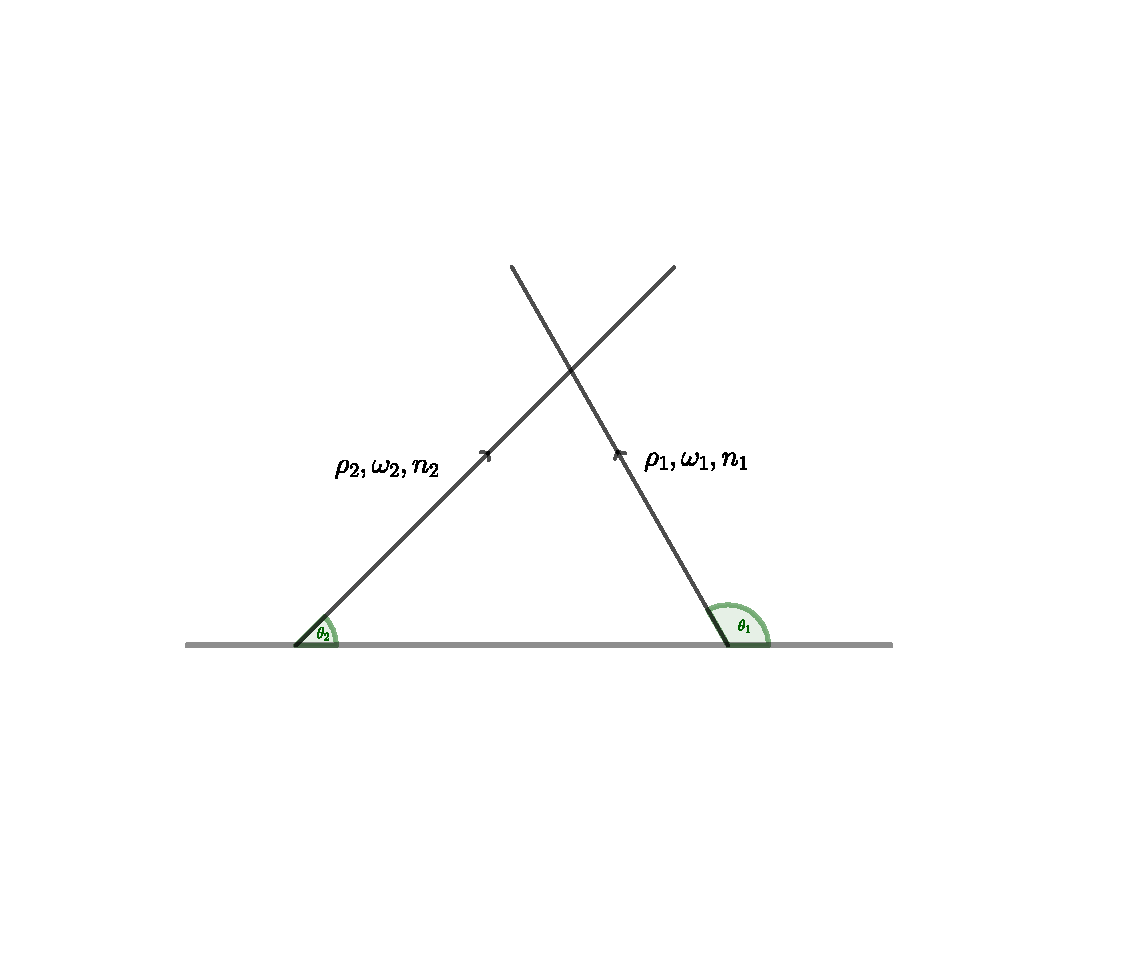
\includegraphics[width=\textwidth]{assets/two-beams-model}
\end{figure}
\end{column}


\end{columns}


\end{frame}


\begin{frame}{Neutrino Self-interactions}

\begin{tcolorbox}
   \only<1>{
   \begin{figure}
      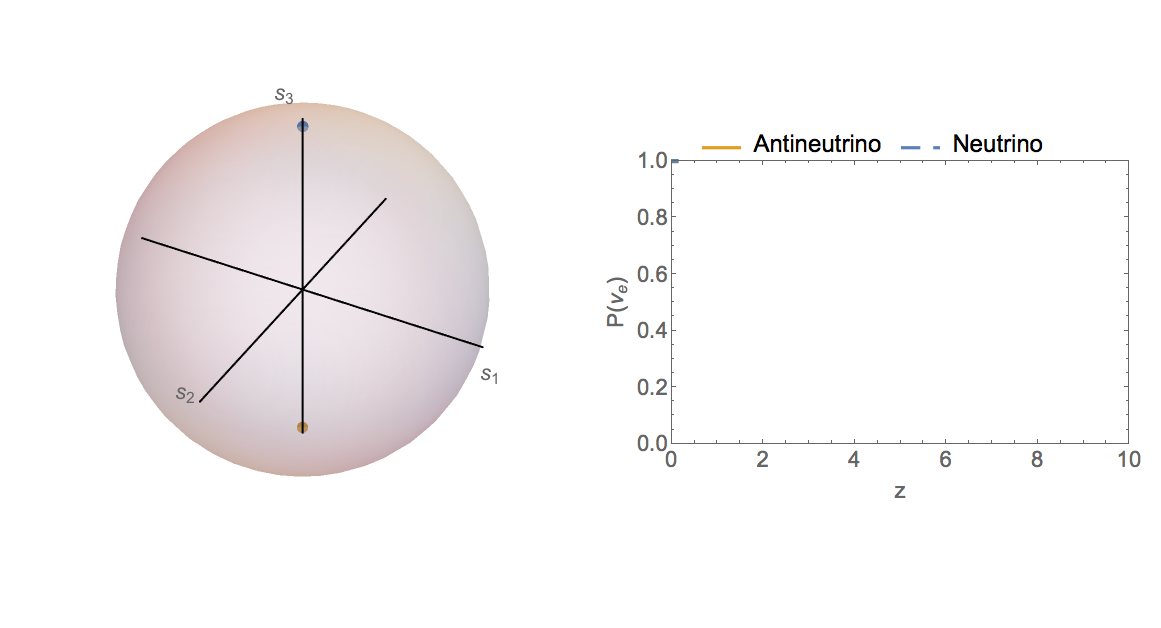
\includegraphics[width=\textwidth]{assets/bipolar-animation/bipolar-animie001.png}
   \end{figure}
   }
   \only<2>{
   \begin{figure}
      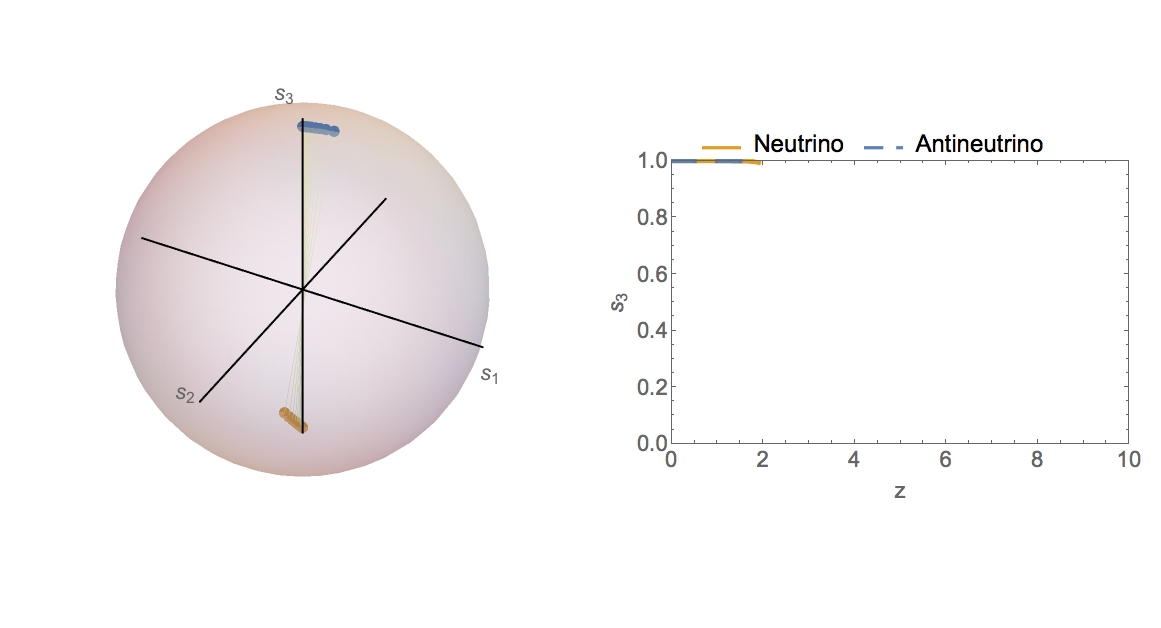
\includegraphics[width=\textwidth]{assets/bipolar-animation/bipolar-animie019.png}
   \end{figure}
   }
   \only<3>{
   \begin{figure}
      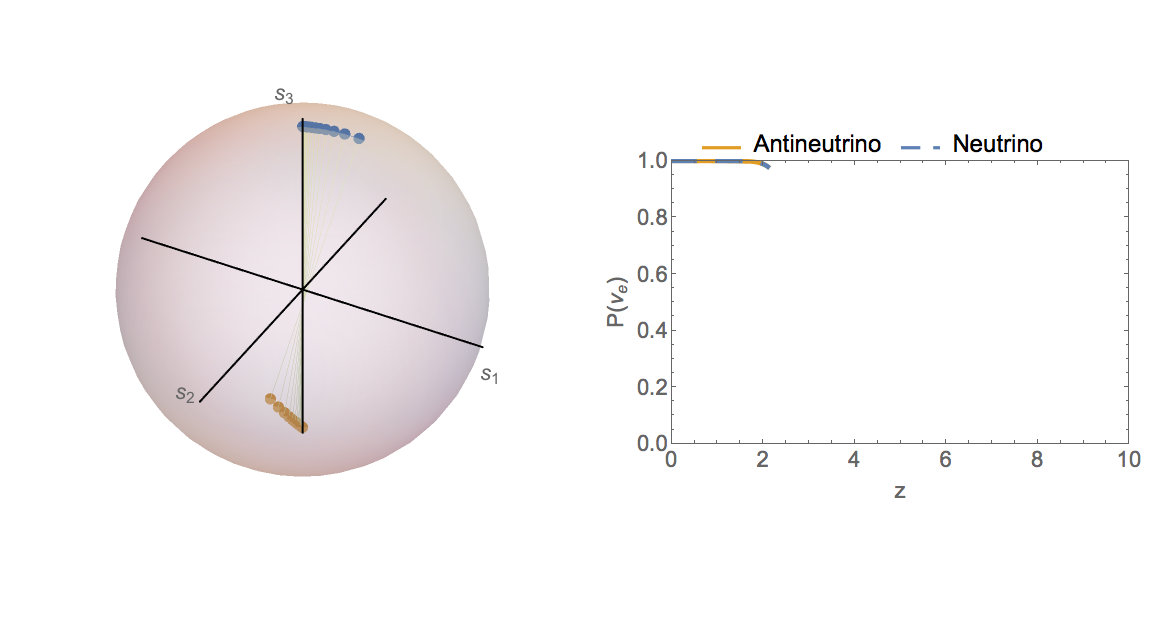
\includegraphics[width=\textwidth]{assets/bipolar-animation/bipolar-animie021.png}
   \end{figure}
   }
   \only<4>{
   \begin{figure}
      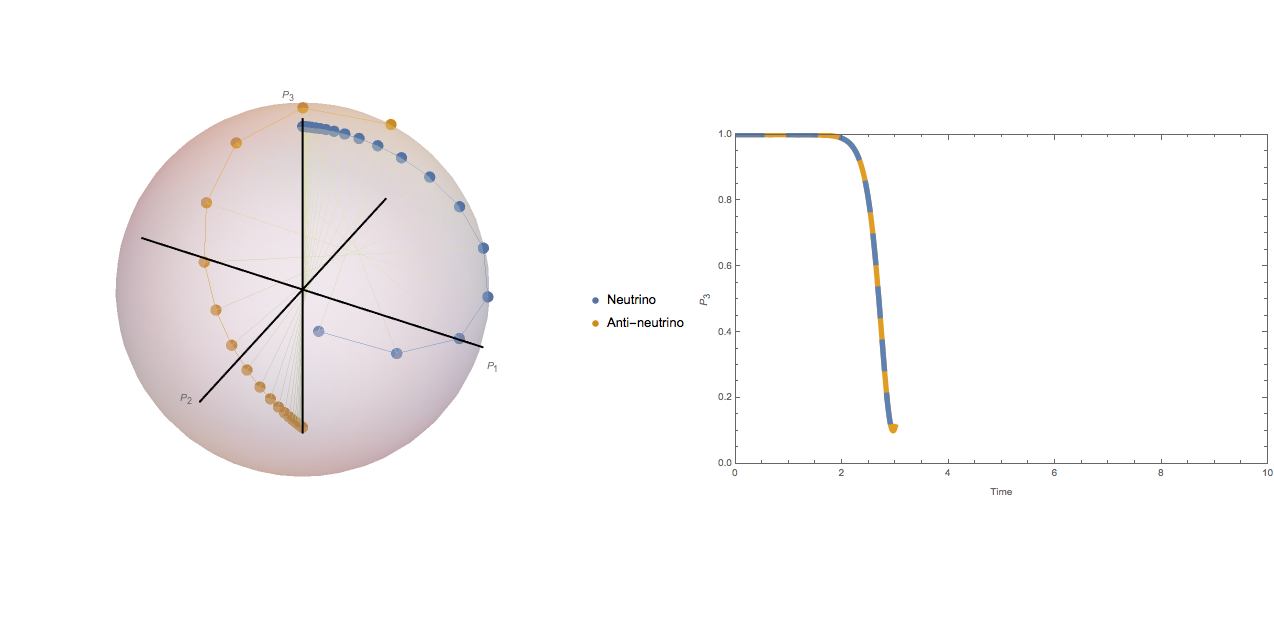
\includegraphics[width=\textwidth]{assets/bipolar-animation/bipolar-animie030.png}
   \end{figure}
   }
   \only<5>{
   \begin{figure}
      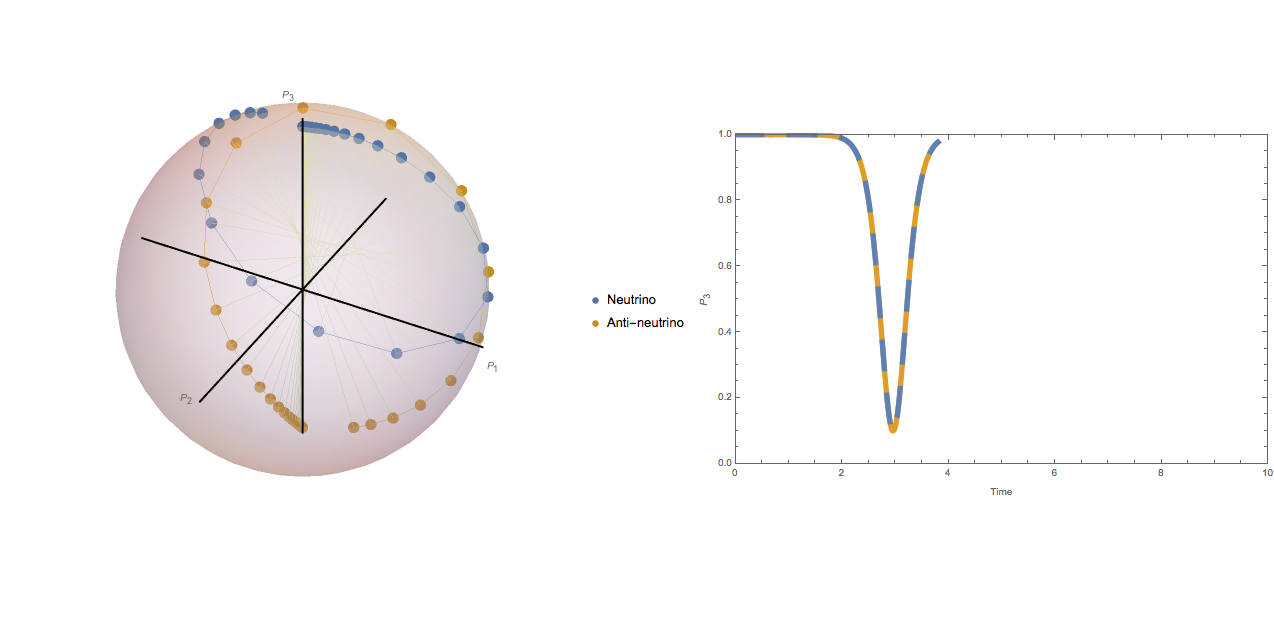
\includegraphics[width=\textwidth]{assets/bipolar-animation/bipolar-animie038.png}
   \end{figure}
   }
   \only<6>{
   \begin{figure}
      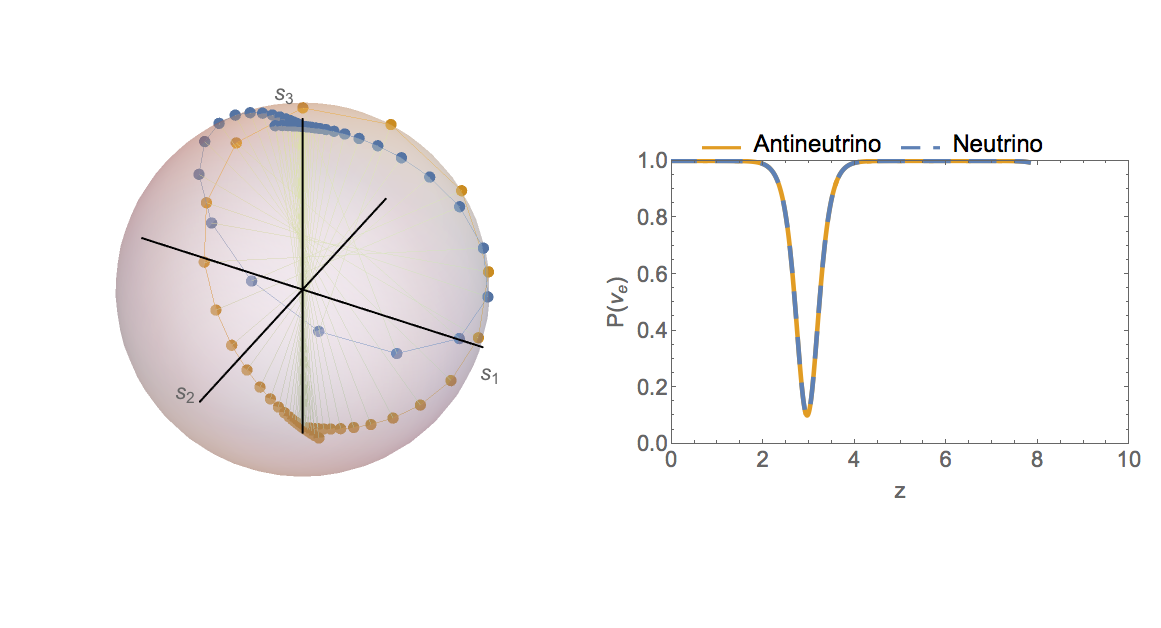
\includegraphics[width=\textwidth]{assets/bipolar-animation/bipolar-animie078.png}
   \end{figure}
   }
   \only<7>{
   \begin{figure}
      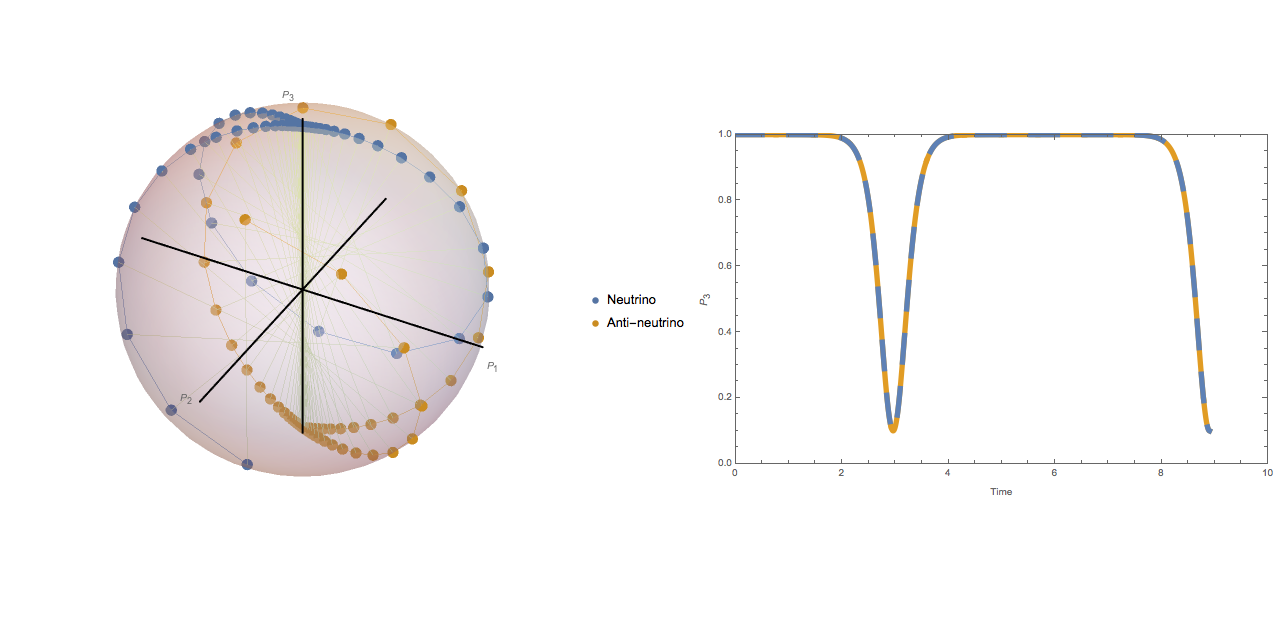
\includegraphics[width=\textwidth]{assets/bipolar-animation/bipolar-animie089.png}
   \end{figure}
   }
   \only<8>{
   \begin{figure}
      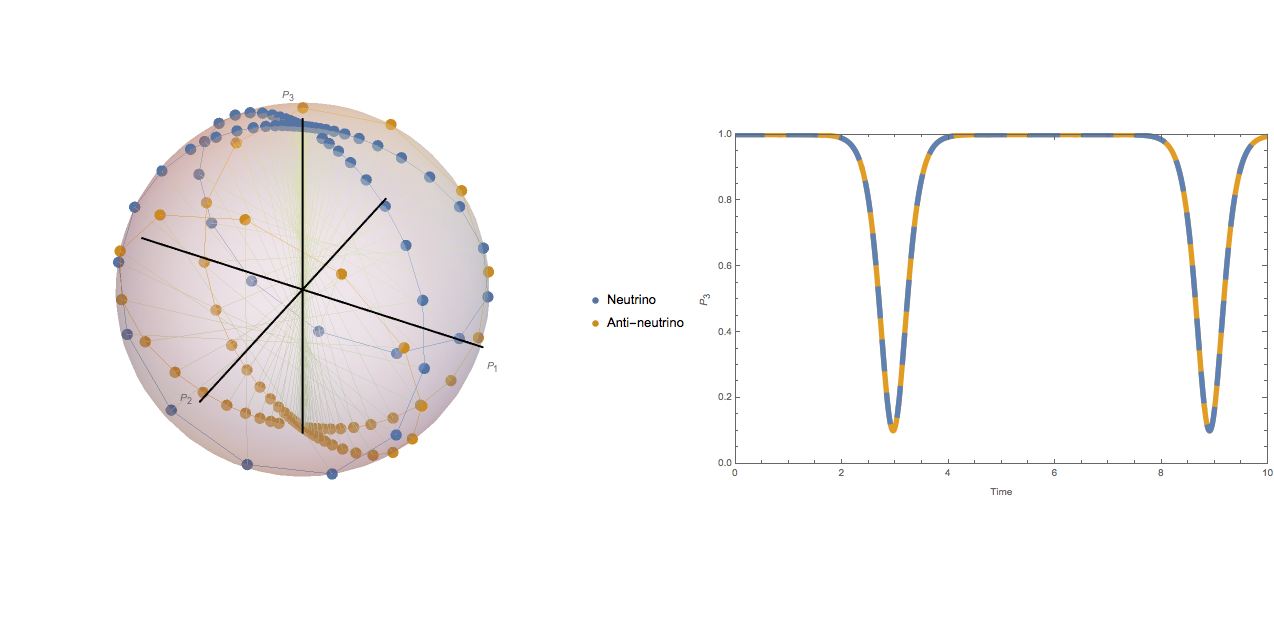
\includegraphics[width=\textwidth]{assets/bipolar-animation/bipolar-animie100.png}
   \end{figure}
   }
\end{tcolorbox}

% \movie[autostart]{Movie}{assets/bipolar-movie.mp4}



\end{frame}



\begin{frame}{Neutrino Self-interactions}


   \begin{tcolorbox}[title=Characteristic Length Scales,standard jigsaw,
    opacityback=0]

      \begin{itemize}
         \item  $\omega_{\mathrm v} = \delta m^2/2E $
         \item  $\lambda \sim G_{\mathrm F} n_e$
         \item  $\mu \sim G_{\mathrm F} (1-\mathbf p_1 \cdot \mathbf p_2) n_{\nu} $
      \end{itemize}

   \end{tcolorbox}


\only<1,2>{


Vacuum oscillation oscillation frequencies
   \begin{align*}
      \omega_{\mathrm v} = \frac{\Delta m^2}{2E}  \sim& \frac{2\pi}{ 1  \mathrm{km} }  \left(\frac{\Delta m^2_{32}}{2.5\times 10^{-3} \mathrm{eV}^2 } \right) \left( \frac{1MeV}{E} \right) \\
   \sim & \frac{2\pi}{ 33  \mathrm{km} } \left( \frac{\delta m_{12}^2}{7.5\times 10^{-5}\mathrm{eV}^2} \right) \left( \frac{1\mathrm{MeV}}{E} \right)
   \end{align*}
}

\only<2>{
\begin{tcolorbox}
   \centering
   Neutrino self-interactions might lead to faster oscillations, since $\mu \gg \omega_{\mathrm v}$.
\end{tcolorbox}
}

\only<3>{

Suppose we have neutrino flux $10^{50}\mathrm{ergs\cdot s^{-1}}$. We estimate the potential at radius $R$ to be

\begin{equation*}
   \mu \sim  \frac{1}{0.01 km} \left(\frac{100\mathrm{km}}{R}\right)^2 \left(\frac{1\mathrm{MeV}}{E}\right)
\end{equation*}


}


\end{frame}





\subsection{Linear Stability Analysis}

\begin{frame}{Linear Stability Analysis}

   \begin{textblock*}{100pt}(220pt,10pt)
   % \textblockcolour{black}
   \TPoptions{showboxes = true }
   \small
   \begin{align*}
      H_{\nu\nu,2} = \frac{1}{2}\mu_1 \rho_1 \xi , \qquad
      H_{\nu\nu,1} = \frac{1}{2}\mu_2 \rho_2 \xi
   \end{align*}
   \end{textblock*}


\begin{columns}[T]



      \begin{column}{0.6\textwidth}
      \begin{figure}
         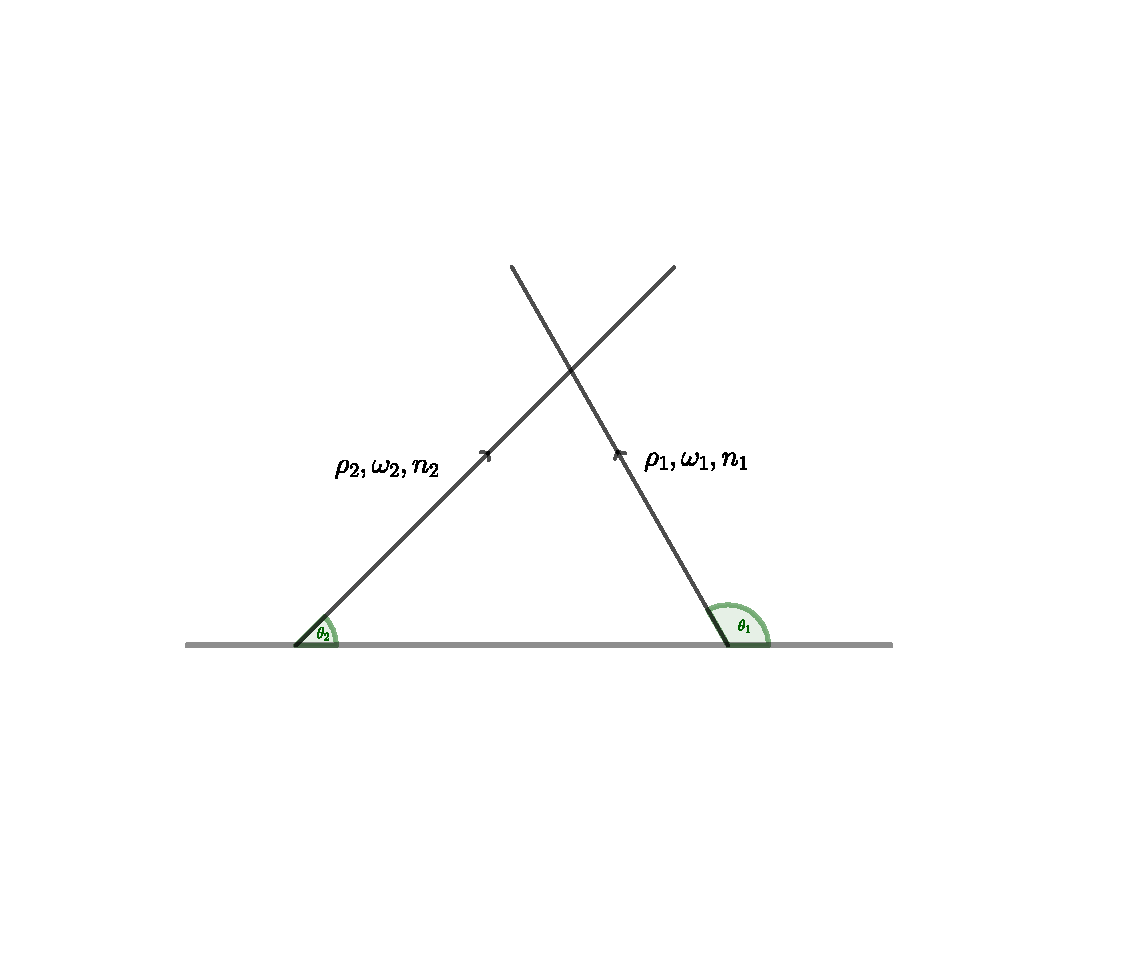
\includegraphics[width=\textwidth]{assets/two-beams-model}
      \end{figure}
      \end{column}

\begin{column}{0.4\textwidth}

$\rho_1$: neutrinos; $\rho_2$: antineutrinos
   \begin{equation*}
   i \partial_z \rho_i = \left[ H_i, \rho_i \right]
   \end{equation*}

   \begin{equation*}
   \theta_1 =  2\pi/3, \theta_2 = \pi/6
   \end{equation*}

\pause

   \begin{align*}
      \rho_i = \frac{1}{2}\begin{pmatrix}
      1 & \epsilon_i\\
      \epsilon_i^* & -1
      \end{pmatrix}
   \end{align*}

\pause


\begin{equation*}
i\partial_{z}\begin{pmatrix}
\epsilon_1 \\
\epsilon_2
\end{pmatrix} = \begin{pmatrix}
\omega_{\mathrm v} - \mu \xi &  \mu  \xi \\
-\mu \xi & -\omega_{\mathrm v} + \mu  \xi
\end{pmatrix}\begin{pmatrix}
\epsilon_1 \\
\epsilon_2
\end{pmatrix}
\end{equation*}


\end{column}


\end{columns}



\end{frame}


\begin{frame}{Linear Stability Analysis}


Eigenvalues

\begin{equation*}
   \pm \sqrt{ \omega_{\mathrm v} ( \omega_{\mathrm v}- 2\mu \xi ) }
\end{equation*}

Identify the condition for complex eigenvalues

\begin{equation*}
   \omega_{\mathrm v} ( \omega_{\mathrm v}- 2\mu \xi ) < 0
\end{equation*}

\pause

\begin{itemize}
   \item Normal hierarchy: $\omega_v>0$, requires $\mu  > \omega_{\mathrm v}/2 \xi$;
   \item Inverted hierarchy: $\omega_v<0$, requires $\mu  < \omega_{\mathrm v}/2 \xi$.
\end{itemize}

\pause

\begin{tcolorbox}
   \centering
   Continuous emission angles?
\end{tcolorbox}

\end{frame}


\subsection{Dispersion Relation}


\begin{frame}{Equation of Motion with Self-interactions}

\begin{equation*}
   i(\partial_t + \hat v )
\end{equation*}

\end{frame}

\begin{frame}{Dispersion Relation}

\begin{equation*}
   \operatorname{Det}(\omega + N^{\nu}_{\phantom{\mu}\nu}) = 0,
\end{equation*}


   \begin{equation*}
      I_n(\theta)=\int_{\cos\theta_2}^{\cos\theta_1} d\cos\theta G(\theta) \frac{\cos^n\theta}{1 - n \cos\theta }
   \end{equation*}


\only<1>{

   \begin{equation*}
      N^\mu_{\phantom{\mu}\nu} = \omega P^\mu_{\phantom{\mu}\nu}\to  \begin{pmatrix}
   \frac{1}{2}  I_0 & 0 & 0 & -\frac{1}{2}I_1\\
   0 & -\frac{1}{4}(I_0-I_2) & 0 & 0\\
   0 & 0 & -\frac{1}{4}(I_0-I_2) & 0 \\
   \frac{1}{2}I_1 & 0 & 0 & -\frac{1}{2}I_2
   \end{pmatrix}
   \end{equation*}
   }


\only<2>{
   \begin{tcolorbox}[title=Solutions]
   \begin{equation*}
   \omega = \frac{1}{4}(I_0-I_2), \quad -\frac{1}{4}\left(I_0-I_2\pm \sqrt{ (I_0-2I_1+I_2)(I_0+2I_1+I_2) }\right)
   \end{equation*}
   \end{tcolorbox}
}

\end{frame}


\begin{frame}{Dispersion Relation}



   \begin{columns}[T]

\begin{column}{0.5\textwidth}
   \begin{figure}
     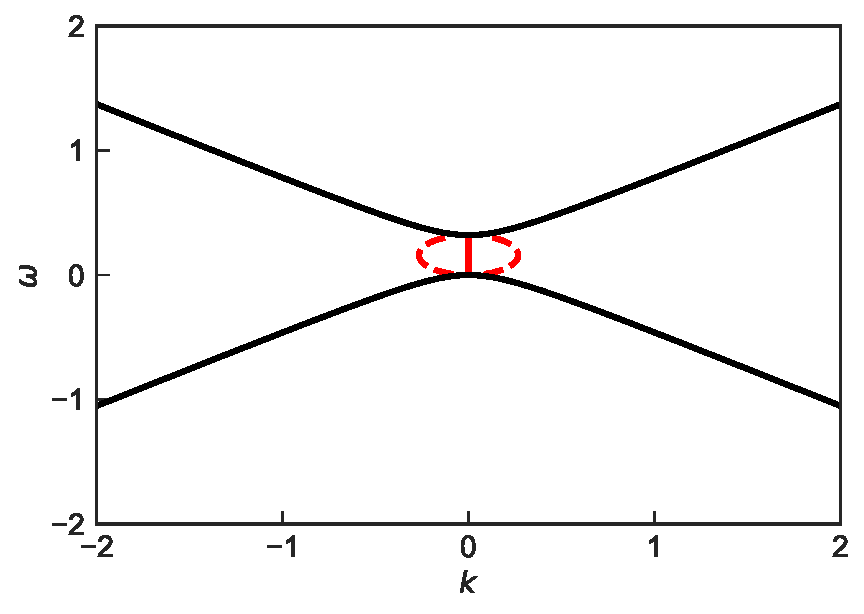
\includegraphics[width=\linewidth]{assets/dr/spectDBWC1DRDBMAAPltBlob.pdf}
     \caption*{MAA solutions}
  \end{figure}
\end{column}

\begin{column}{0.5\textwidth}
   \begin{figure}
      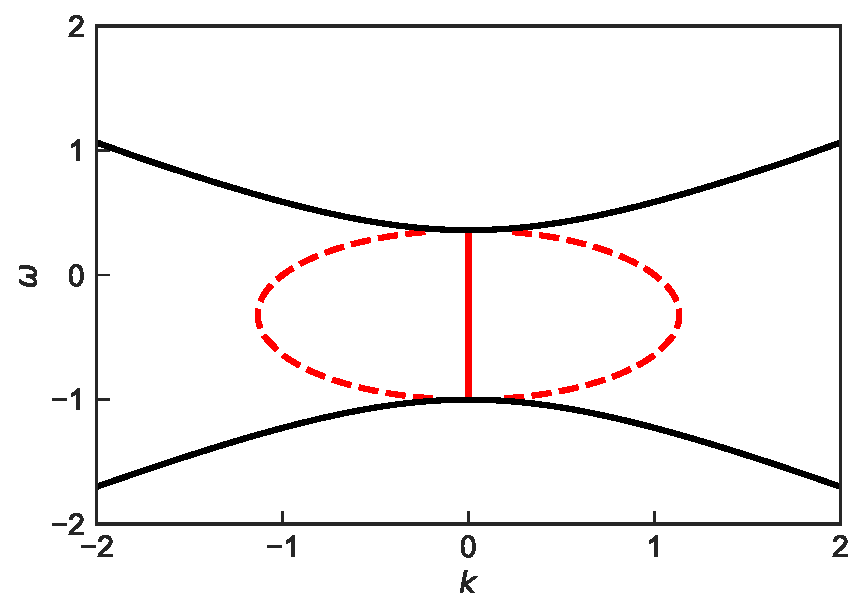
\includegraphics[width=\linewidth]{assets/dr/spectDBWC1DRDBMZAPltBlob.pdf}
      \caption*{ MZA solutions}
   \end{figure}
\end{column}

   \end{columns}

\begin{tcolorbox}
   \centering
   Two beams
\end{tcolorbox}

\end{frame}

\begin{frame}{Dispersion Relation}



   \begin{columns}[T]

\begin{column}{0.5\textwidth}
   \begin{figure}
     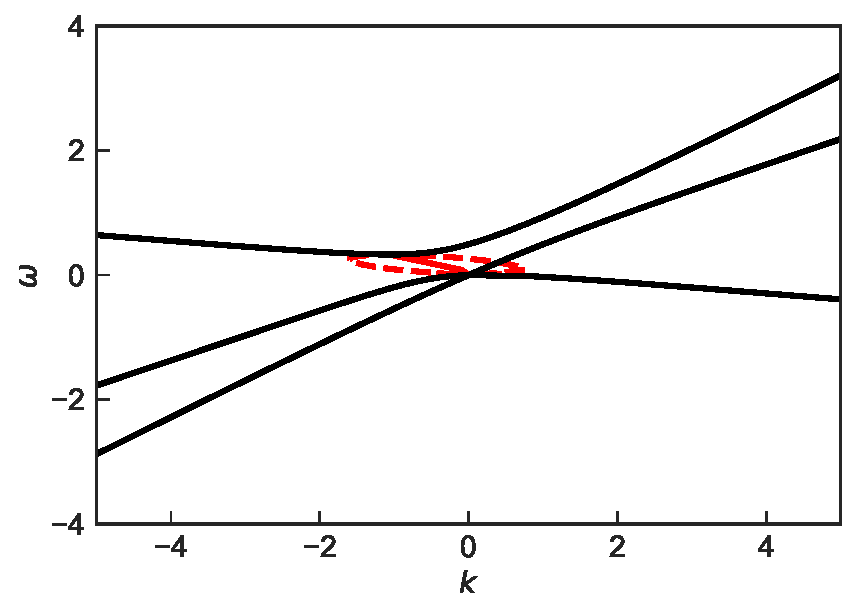
\includegraphics[width=\linewidth]{assets/dr/spectDB3WC4DRDBMAAPltBlob.pdf}
     \caption*{MAA solutions}
  \end{figure}
\end{column}

\begin{column}{0.5\textwidth}
   \begin{figure}
      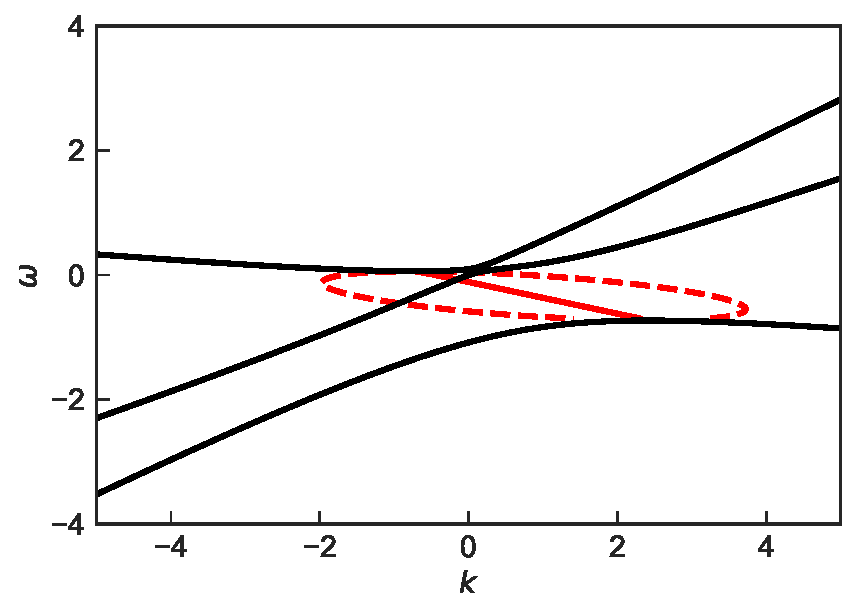
\includegraphics[width=\linewidth]{assets/dr/spectDB3WC4DRDBMZAPltBlob.pdf}
      \caption*{ MZA solutions}
   \end{figure}
\end{column}

   \end{columns}

   \begin{tcolorbox}
      \centering
      Three beams
   \end{tcolorbox}


\end{frame}


\begin{frame}{Dispersion Relations}

   \begin{figure}
      \minipage{0.49\textwidth}
        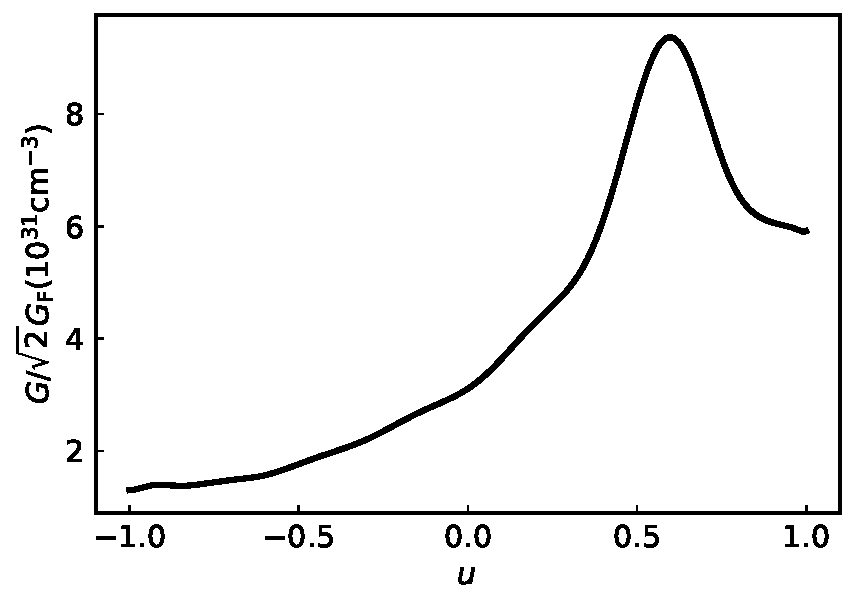
\includegraphics[width=\linewidth]{assets/dr/spectGarchingPlt.pdf}
      \endminipage\hfill
      \minipage{0.49\textwidth}
      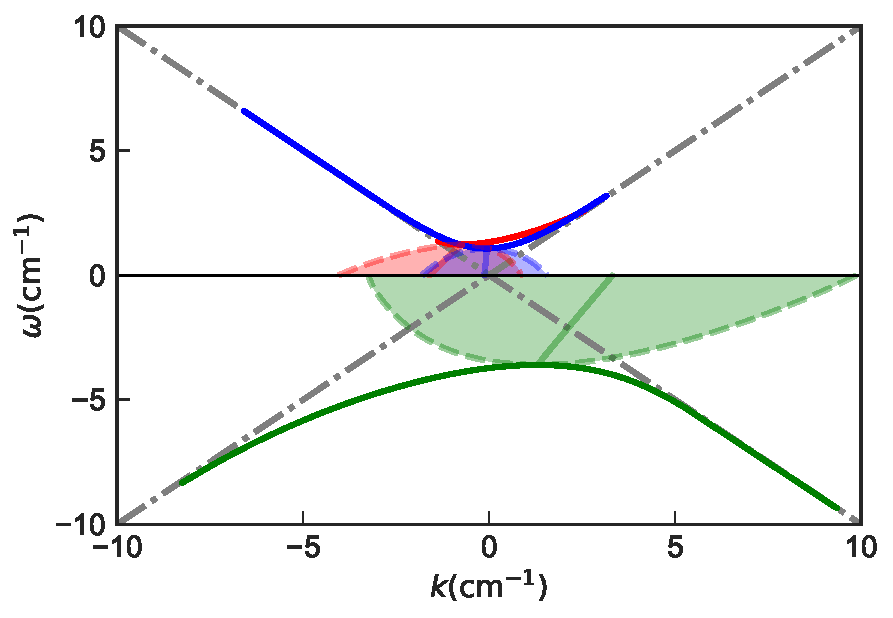
\includegraphics[width=\linewidth]{assets/dr/spectGarchingDRLSAPltBlob.pdf}
      \endminipage\hfill
      \caption*{Dispersion relation and linear stability analysis (right panel) for a spectrum constructed from Garching 1D simulation data (left panel). Solid red line is dispersion relation for MAA solution while blue and green lines are for MZA solutions. Light red (green and green) blob is instability for MAA (MZA) solution.
       }
   \end{figure}


\end{frame}

\begin{frame}{Dispersion Relations}

\begin{equation*}
   k = \frac{1}{4} \int \mathrm du G(u) \frac{ 1 - u^2 }{ \omega/k - u }.
   \label{eqn-k-omega-relation}
\end{equation*}


\begin{align*}
\operatorname{Re}(k) =& \frac{1}{4}\left(  \mathcal{P} \int \mathrm d u G(u) \frac{ 1 - u^2 }{ - u }  \right)\label{eqn-re-k-arbitrary-spectrum} \\
\operatorname{Im}(k) =&  \frac{\pi}{4}G(0) \operatorname{Sign}\left( \omega \right) \operatorname{Sign}\left(  \operatorname{Im}(k)  \right).
\end{align*}

\begin{equation*}
   \lvert \operatorname{Im}(k) \rvert  =  \frac{\pi}{4}\lvert G(0)\rvert .
\end{equation*}



\begin{align*}
&\left(4\operatorname{Re}(k) - \mathcal P \int \frac{G(u)}{u} \mathrm d u + U_1 \right)^2  - \left( \operatorname{Sign}(\omega \operatorname{Im}(k) )\pi G(0) +4 \operatorname{Im}(k) \right)^2 \\
=& - \left( \mathcal P \int \frac{G(u)}{u} \mathrm du + U_1 \right) \pi \operatorname{Sign}(\omega \operatorname{Im}(k) ) G(0),
\end{align*}

% \begin{equation*}
%    \operatorname{Im}(k) = - \frac{1}{4} \pi G(0) \operatorname{Sign}(\omega \operatorname{Im}(k) ) \left(  1 \pm \frac{ \mathscr P \int \frac{G(u)}{u} du + \int G(u) u du }{ 4 \operatorname{Re}(k) - \mathscr P \int \frac{G(u)}{u} du + \int G(u) u du }  \right)
% \end{equation*}

\end{frame}



\begin{frame}{Dispersion Relations}

   \begin{figure}
      \minipage{0.49\textwidth}
      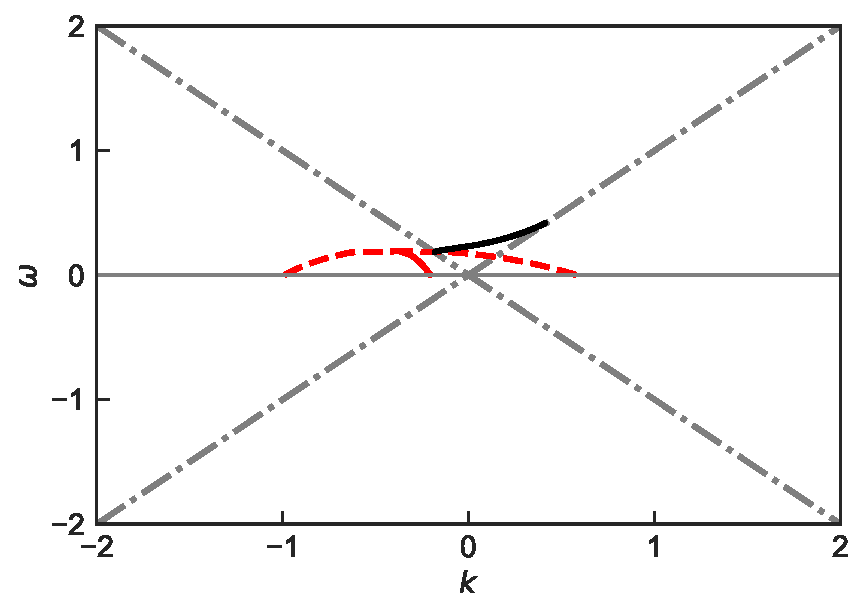
\includegraphics[width=\linewidth]{assets/dr/spectBoxC1MAADRPltBlob.pdf}
      \endminipage\hfill
      \minipage{0.49\textwidth}
      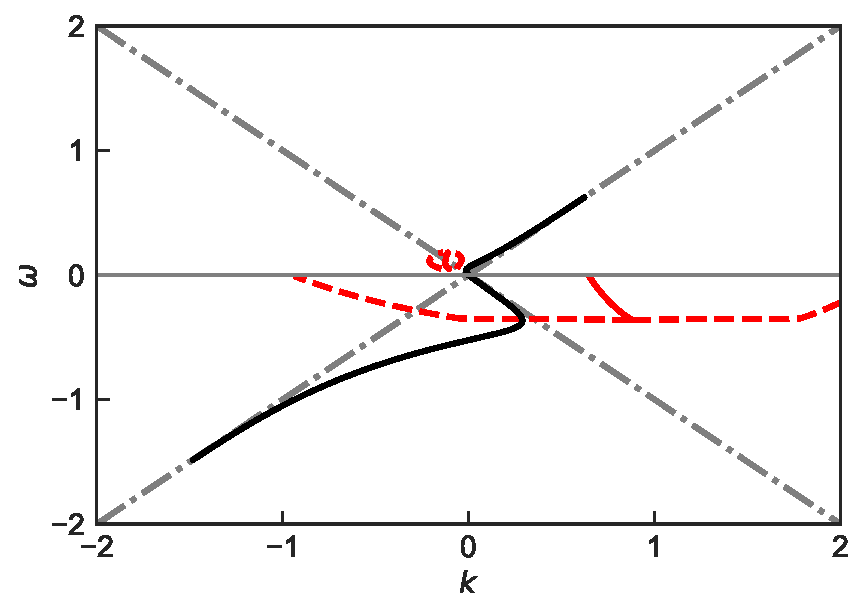
\includegraphics[width=\linewidth]{assets/dr/spectBoxC1MZADRPltBlob.pdf}
      \endminipage\hfill
      \caption*{Dispersion relation and linear stability analysis for box spectrum. The box spectrum is defined to be $-0.1$ within range $u\in [-1,-0.3)$ and $1$ within range $u\in [-0.3,1]$. Left panel shows the dispersion relation and the complex $k$ for real $\omega$ for MAA solution. Right panel is the corresponding result for MZA solution. Dash-dotted gray lines are $\omega= \pm k$ which sets the boundaries of the forbidden region for dispersion relation.
       }
   \end{figure}



\end{frame}






%%%%%%%%%%%%%%%%%%%%%%%%%%%%%%%%%%%%%%%%%%%%%%%%%%%%%%%
%%%%%%% Summary


\section{Summary}

\begin{frame}{Summary}



\begin{itemize}\color{ao}
\item
The fact that neutrino flavor sates are not mass states causes vacuum oscillations.
\item
MSW resonance happens when matter potential cancels out the vacuum diagonal elements of the Hamiltonian.
\item
Even matter profile doesn't match MSW requirement, variation in matter profile can cause resonances.
\item
Single frequency perturbations in matter profile is a combination of many Rabi oscillations.
\end{itemize}



\begin{itemize}\color{red}
 \item
 How to understand and calculate systems with multi-frequency matter profile (turbulence).
 \item
 Combine periodic or even turbulent matter profile with neutrino self-interaction.
\end{itemize}




\end{frame}



\begin{frame}{Acknowledgement}

I am very thankful to my advisor Professor Huaiyu Duan, Dr. Sajad Abbar, and Dr. Shashank Shalgar, and Joshua Martin, for all the help in both research and life.

Supported by DOE EPSCoR grant \#DE-SC0008142 at UNM.

\end{frame}






    \begin{frame}[label=citations]{Citations}
      \framesubtitle{\TeX, \LaTeX, and Beamer}

      \justifying\TeX\ is a programming language for the typesetting
      of documents. It was created by Donald Erwin Knuth in the late
      1970s and it is documented in \emph{The \TeX
      book}~\cite{knuth84}.

      In the early 1980s, Leslie Lamport created the initial version
      of \LaTeX, a high-level language on top of \TeX, which is
      documented in \emph{\LaTeX : A Document Preparation
      System}~\cite{lamport94}. There exists a healthy ecosystem of
      packages that extend the base functionality of \LaTeX;
      \emph{The \LaTeX\ Companion}~\cite{MG94} acts as a guide
      through the ecosystem.

      In 2003, Till Tantau created the initial version of Beamer, a
      \LaTeX\ package for the creation of presentations. Beamer is
      documented in the \emph{User's Guide to the Beamer
      Class}~\cite{tantau04}.
    \end{frame}

    \begin{frame}[label=bibliography]{Bibliography}
      \framesubtitle{\TeX, \LaTeX, and Beamer}
      \begin{thebibliography}{9}
        \bibitem{knuth84}
            Donald~E.~Knuth.
            \emph{The \TeX book}.
            Addison-Wesley, 1984.
        \bibitem{lamport94}
            Leslie~Lamport.
            \emph{\LaTeX : A Document Preparation System}.
            Addison-Wesley, 1986.
        \bibitem{MG94}
            M.~Goossens, F.~Mittelbach, and A.~Samarin.
            \emph{The \LaTeX\ Companion}.
            Addison-Wesley, 1994.
        \bibitem{tantau04}
            Till~Tantau.
            \emph{User's Guide to the Beamer Class Version 3.01}.
            Available at \url{http://latex-beamer.sourceforge.net}.
        \bibitem{MS05}
            A.~Mertz and W.~Slough.
            Edited by B.~Beeton and K.~Berry.
            \emph{Beamer by example} In TUGboat,
              Vol. 26, No. 1., pp. 68-73.
      \end{thebibliography}
    \end{frame}

  \end{darkframes}



\appendix


\begin{frame}

\begin{tcolorbox}
   \centering
   Backup Slides
\end{tcolorbox}

\end{frame}

\begin{frame}{Hamiltonian, and Basis, and Rabi Oscillations}



\begin{tcolorbox}[title=Hamiltonian in Background Matter Basis]
    \begin{equation*}
    \mathbf {H} = \frac{1}{2}\left( - \omega_{\mathrm{m}} + {\color{red}\delta \lambda(x)} \cos 2\theta_{\mathrm{m}} \right) \sigma_3 - \frac{  {\color{red}\delta \lambda(x)}  }{2} \sin 2\theta_{\mathrm{m}} \sigma_1.
\end{equation*}
\end{tcolorbox}


Matter profile
\begin{equation*}
    \lambda(x) = \lambda_0 + {\color{red}A \cos (k x)},
\end{equation*}


\begin{equation*}
    \mathbf {H} = \frac{1}{2}\left( - \omega_{\mathrm{m}} +  \cos 2\theta_{\mathrm{m}}{\color{red}A\cos(kx)} \right) \sigma_3 - \frac{  \sin 2\theta_{\mathrm{m} }  }{2}{\color{red}A \cos(kx)}  \sigma_1.
\end{equation*}





\end{frame}


\begin{frame}{Stimulated Neutrino Oscillations}


\only<1-1>{
% Matter profile
\begin{tcolorbox}[title=Matter Profile]
\begin{equation*}
    \lambda(x)  = \lambda_0 + {\color{red}\delta\lambda(x)}
\end{equation*}
\end{tcolorbox}


% Basis


\begin{tcolorbox}[title=Basis]

Background matter basis: Hamiltonian is diagonalized with only background matter profile $\lambda_0$,

\begin{equation*}
    \mathrm{H}_{\mathrm{background}} = -\frac{\omega_{\mathrm{m}}}{2} \boldsymbol{\sigma_3}.
\end{equation*}

\end{tcolorbox}


% Hamiltonian of with perturbation in matter profile, in background matter basis
\begin{tcolorbox}[title=Hamiltonian]

\begin{equation*}
    \mathbf H = \frac{1}{2}\left( - \omega_{\mathrm{m}} + {\color{red}\delta \lambda(x)} \cos 2\theta_{\mathrm{m}} \right) \boldsymbol{\sigma_3} - \frac{{\color{red}\delta \lambda(x) } }{2} \sin \theta_{\mathrm{m}} \boldsymbol{\sigma_1}.
\end{equation*}


\end{tcolorbox}

}

\only<2-2>{

% \begin{tcolorbox}
% Kneller, J. P., McLaughlin, G. C., \& Patton, K. M. (2013). J. Phys. G: Nucl. Part. Phys. {\bf{40}} (2013) 055002.
% \end{tcolorbox}

\begin{tcolorbox}
P. Krastev and A. Smirnov (1989); J. Kneller et al (2013);\\ K. Patton et al (2014);
\end{tcolorbox}


\begin{figure}
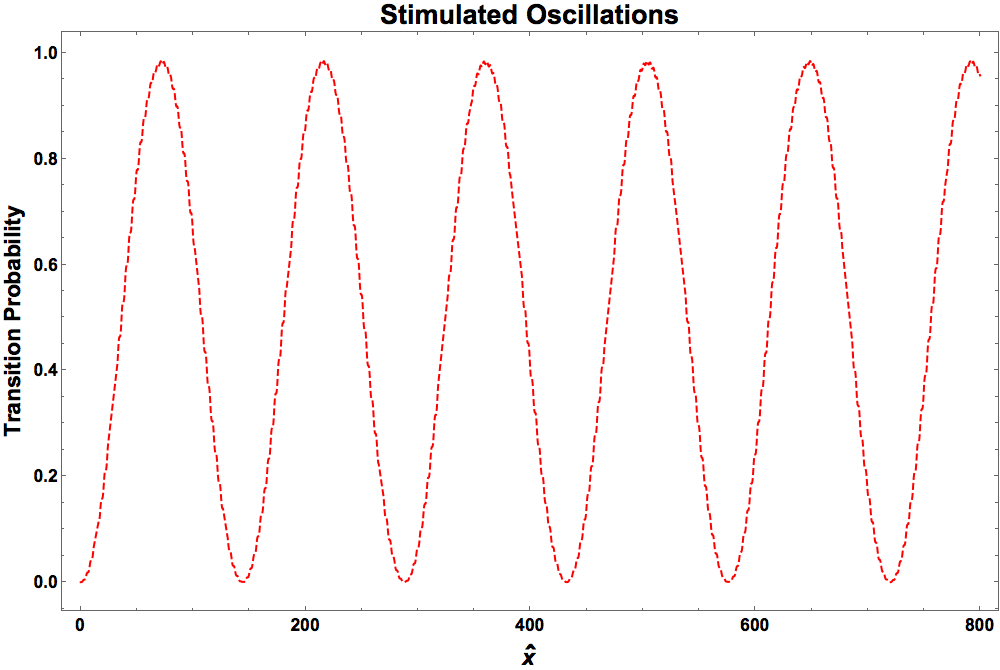
\includegraphics[width=0.8\textwidth]{assets/stimulated-oscillation-phenomenon.png}
%stimulated-neutrino-oscillations-kneller.png}
\caption*{Stimulated oscillations. $\lambda(x) = \lambda_0 +  A \sin (k x)$  with $\hat x = \omega_{\mathrm m} x $, $A=0.1\omega_{\mathrm m}$, $k=0.995\omega_{\mathrm m}$, $\theta_{\mathrm{m}}=\pi/6$}
\end{figure}


}





\end{frame}







%%%%%%%%%%%%%%%%%%%%%%%%%%%%%%
%%%% Neutrino Halo Problem






\begin{frame}{Neutrino Halo}

\only<1>{
\begin{figure}
   \includegraphics[width=\textwidth]{assets/halo-line-model}
\end{figure}
}

\only<2>{

\begin{columns}[T]
   \begin{column}{0.5\textwidth}
      Assumptions
      \begin{itemize}
         \item Neutrinos are translational symmetric on the emission line.
         \item Reflection obays Snell's law.
         \item Neutrinos are reflected on a fixed surface $z=L$.
         \item Neutrino reflections are translational symmetric.
      \end{itemize}

   \end{column}

   \begin{column}{0.5\textwidth}
      \begin{figure}
         \includegraphics[width=\textwidth]{assets/halo-line-model}
      \end{figure}
   \end{column}
\end{columns}


}

\end{frame}

\subsection{Flavor Isospin Picture}

\begin{frame}{Flavor Isospin}


\begin{figure}
   \includegraphics[width=\textwidth]{assets/halo-line-model-single-beam}
\end{figure}


\end{frame}



\begin{frame}{Relaxation Scheme}

\begin{tcolorbox}[title=Algorithm,standard jigsaw,
    opacityback=0]
   \begin{enumerate}
      \item Calculate forward beam using null backward beam;
      \item Calculate backward beam using forward beam calculated in step 1;
      \item Calculate forward beam using backward beam calculated in step 2;
      \item Repeat 2 and 3 until the beams reach equilibrium.
   \end{enumerate}
\end{tcolorbox}




\end{frame}




\begin{frame}{Numerical Method}

\begin{tcolorbox}
\begin{figure}
   \includegraphics[width=0.9\textwidth]{assets/relax-color}
   \caption*{\color{black}Horizontal axis is the location of neutrinos; Vertical axis is the number of iteration steps; Color indicates the electron flavor probability.}
\end{figure}
\end{tcolorbox}

\end{frame}


\begin{frame}{Numerical Method}

\begin{tcolorbox}
   \begin{figure}
      \includegraphics[width=\textwidth]{assets/halo-mu-4-r-multiple}
   \end{figure}
\end{tcolorbox}

\end{frame}

\begin{frame}{Linear Stability Analysis}

EoM

   \begin{align*}
    i \partial_t \vec s_F &= \mathbf s_F \times (\vec {H}_v +R \mu \vec s_B) \\
      i\partial_t \vec s_B &= \vec s_B \times (- \vec H_v - \mu \vec s_F) .
   \end{align*}

Compare with bipolar

\begin{align*}
    i\partial_t \vec s &= \mathbf s \times ( \eta \vec H_v + \alpha \mu \bar{\vec s} )\\
    i\partial_t \bar{\vec s} &= \bar{\vec s} \times ( \eta \vec H_v + \mu \vec s )
\end{align*}


\end{frame}


\begin{frame}{Linear Stability Analysis}


\begin{tcolorbox}

   % \only<1>{
      \begin{figure}
         \includegraphics[width=\textwidth]{assets/halo-mu-1-reflection-0p07}
      \end{figure}
      % }

   % \only<2>{
   %    \begin{figure}
   %       \includegraphics[width=\textwidth]{assets/halo-mu-4-compare-bipolar}
   %    \end{figure}
   % }

\end{tcolorbox}



\end{frame}






\end{document}
